
\title{Lab Report 06 - Stereo Matching}
\author{
        Manuel Galliker  14-921-969 \\
                manuelga@student.ethz.ch
}
\date{\today}

\documentclass[12pt]{article}
\usepackage{graphicx}
\usepackage{float}
\begin{document}
\maketitle


\section{1. Disparity Computation}

In the first part of this exercise a winner-takes-all stereo matching algorithm was implemented. It uses SSD (Sum of Squared Distances). First the functions $imgRectL$ and $imgRectR$ are used to project the images onto a single plane. This would correspond with only a translation in horizontal ($x$) direction two cameras at the same height above ground. 
\newline 
Since the orientation of the two cameras is identical the epi-poles lie at infinity and the epi-lines are parallel and horizontal. From this we know that from a point $a$ in the first image a corresponding point $a'$ in the second image can be obtained by a translation in $x$ direction from the cordinate of point $a$. 
\newline 
Then The implemented algorithm uses a range of pixels (by default $[-40, 40]$) to shift the second image in $x$ direction for the hole range. For each shift the difference between the two filtered images is calculted and then filtered by an average filter using an aeria $filter_window_size$ and the functions $fspecial$ and $imfilter$. Where then this difference is smallest its assumed to have found a good matching point and the distance the point is shifted is stored in the disparity map.  

\vspace{5mm}
\begin{figure}[H]
	\centering
	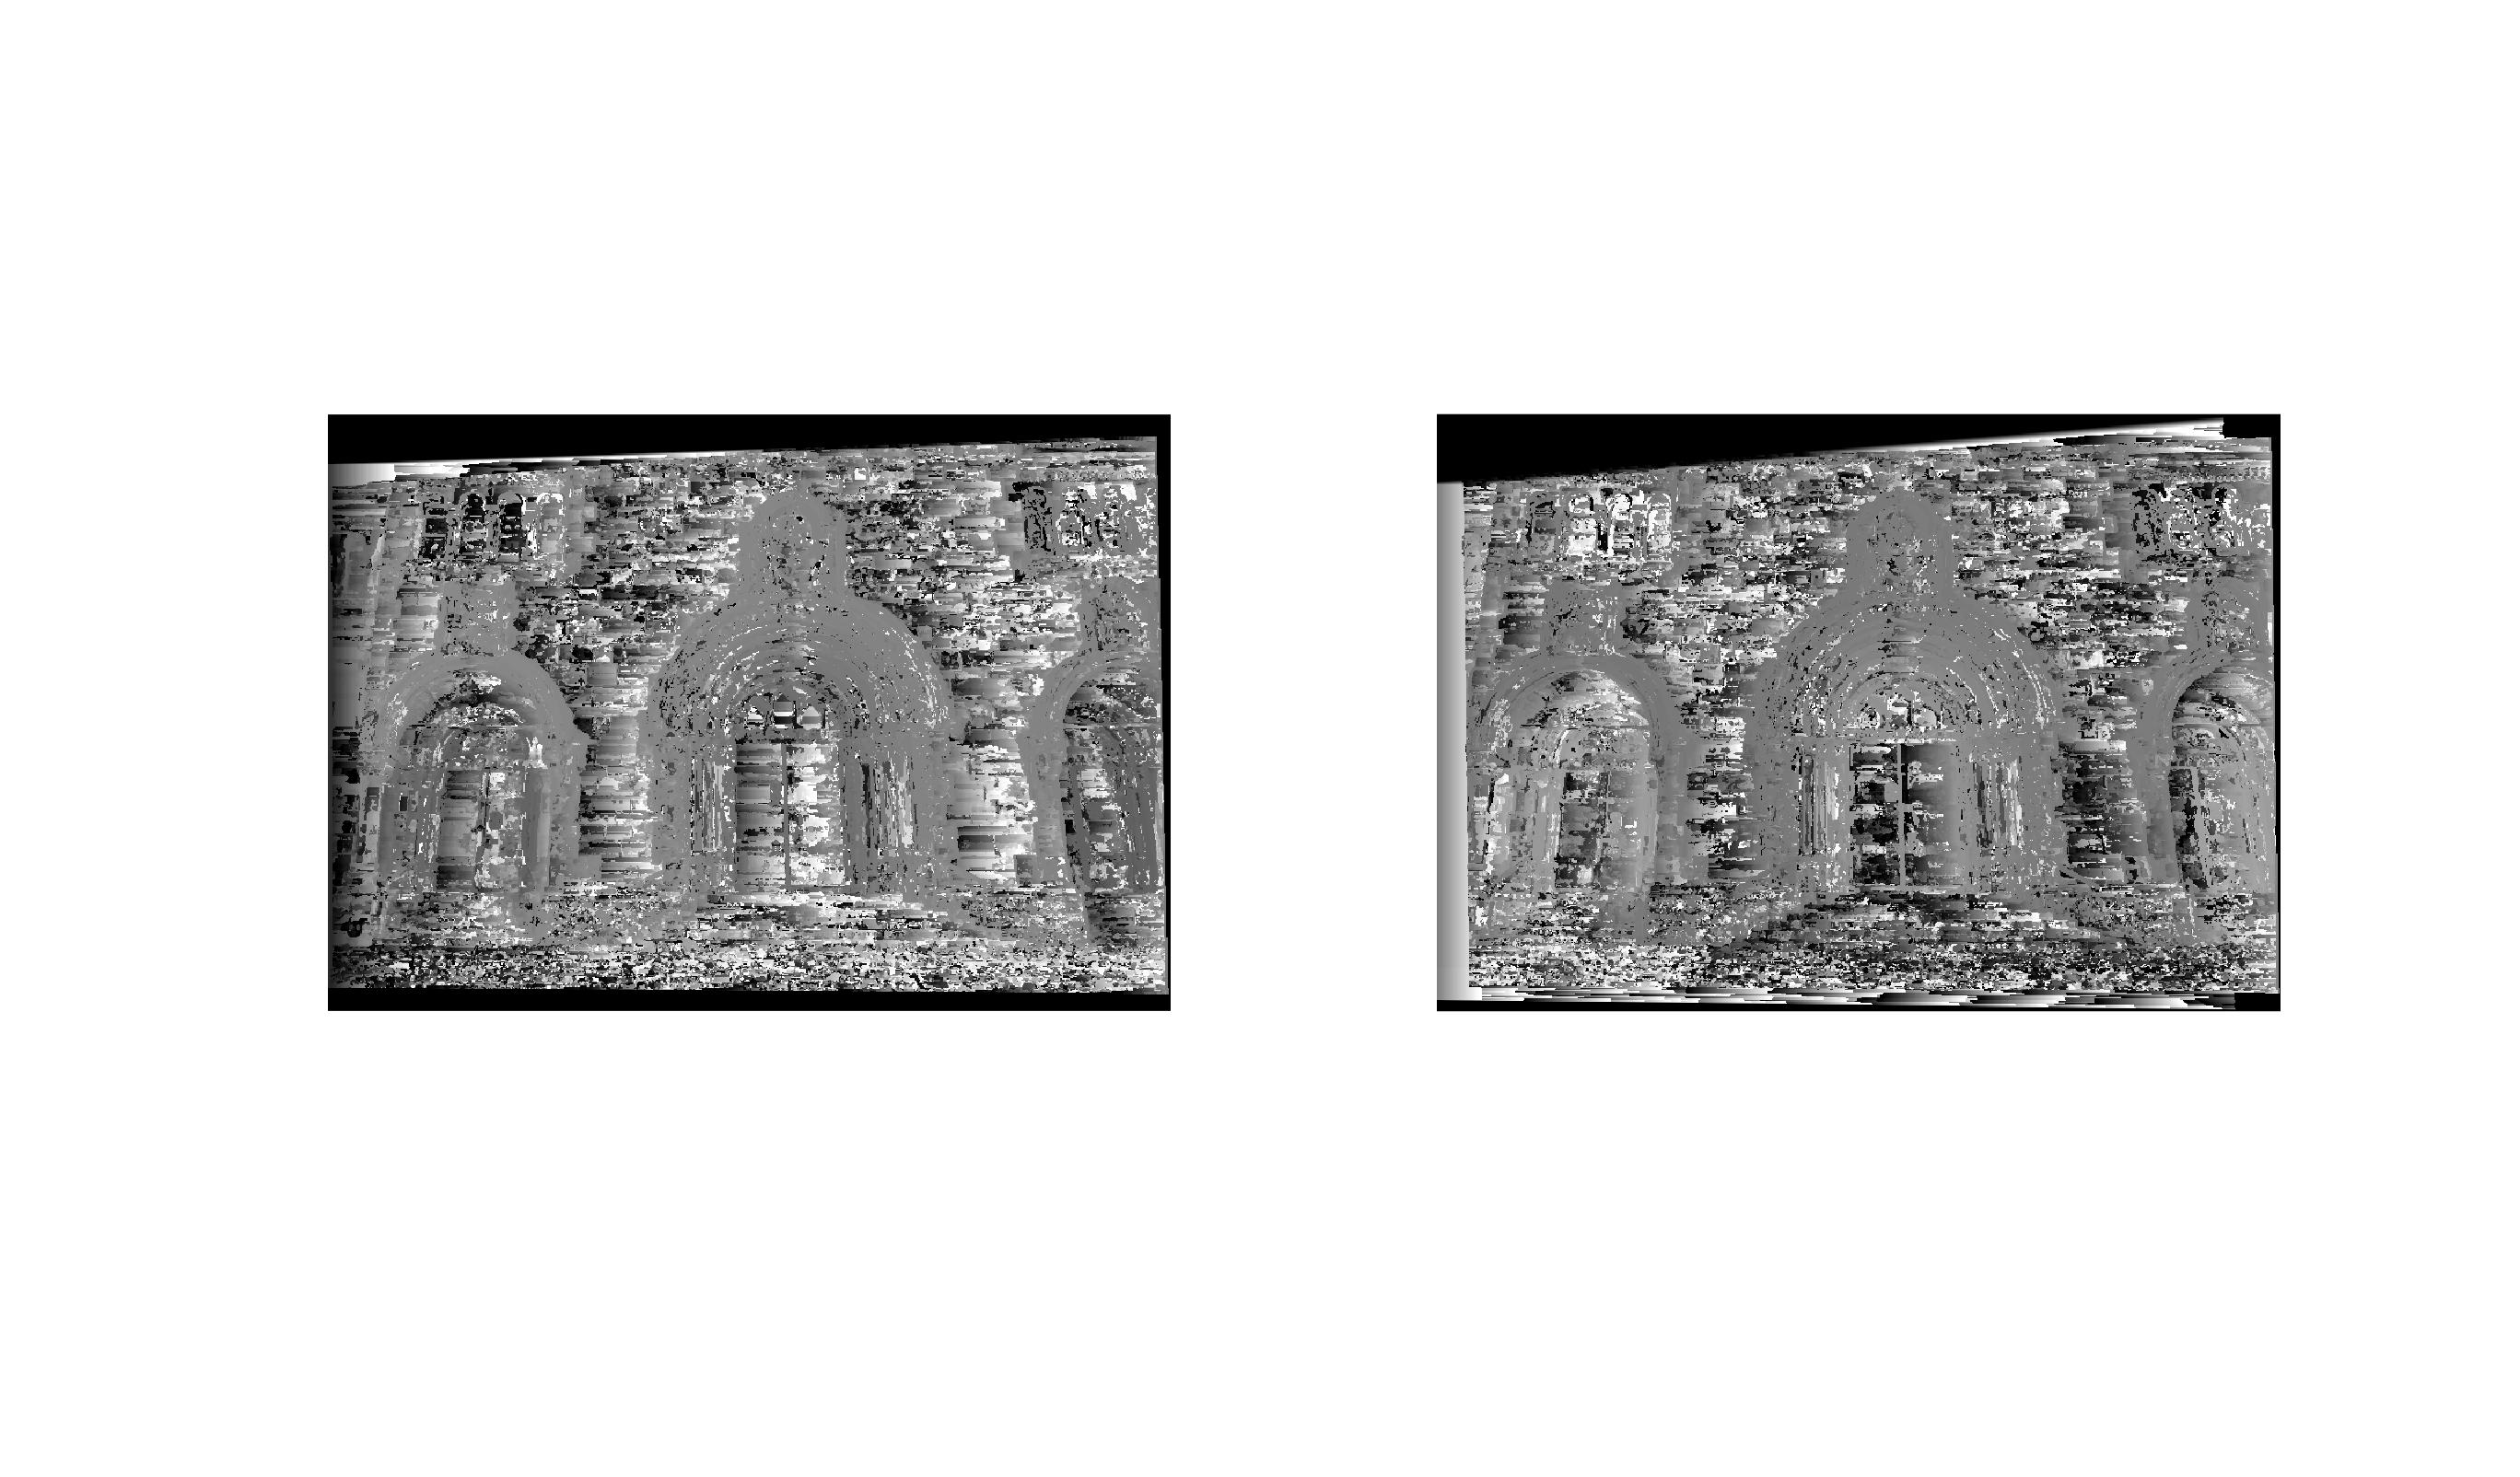
\includegraphics[width=1.1\textwidth]{dc3_1.jpg}
	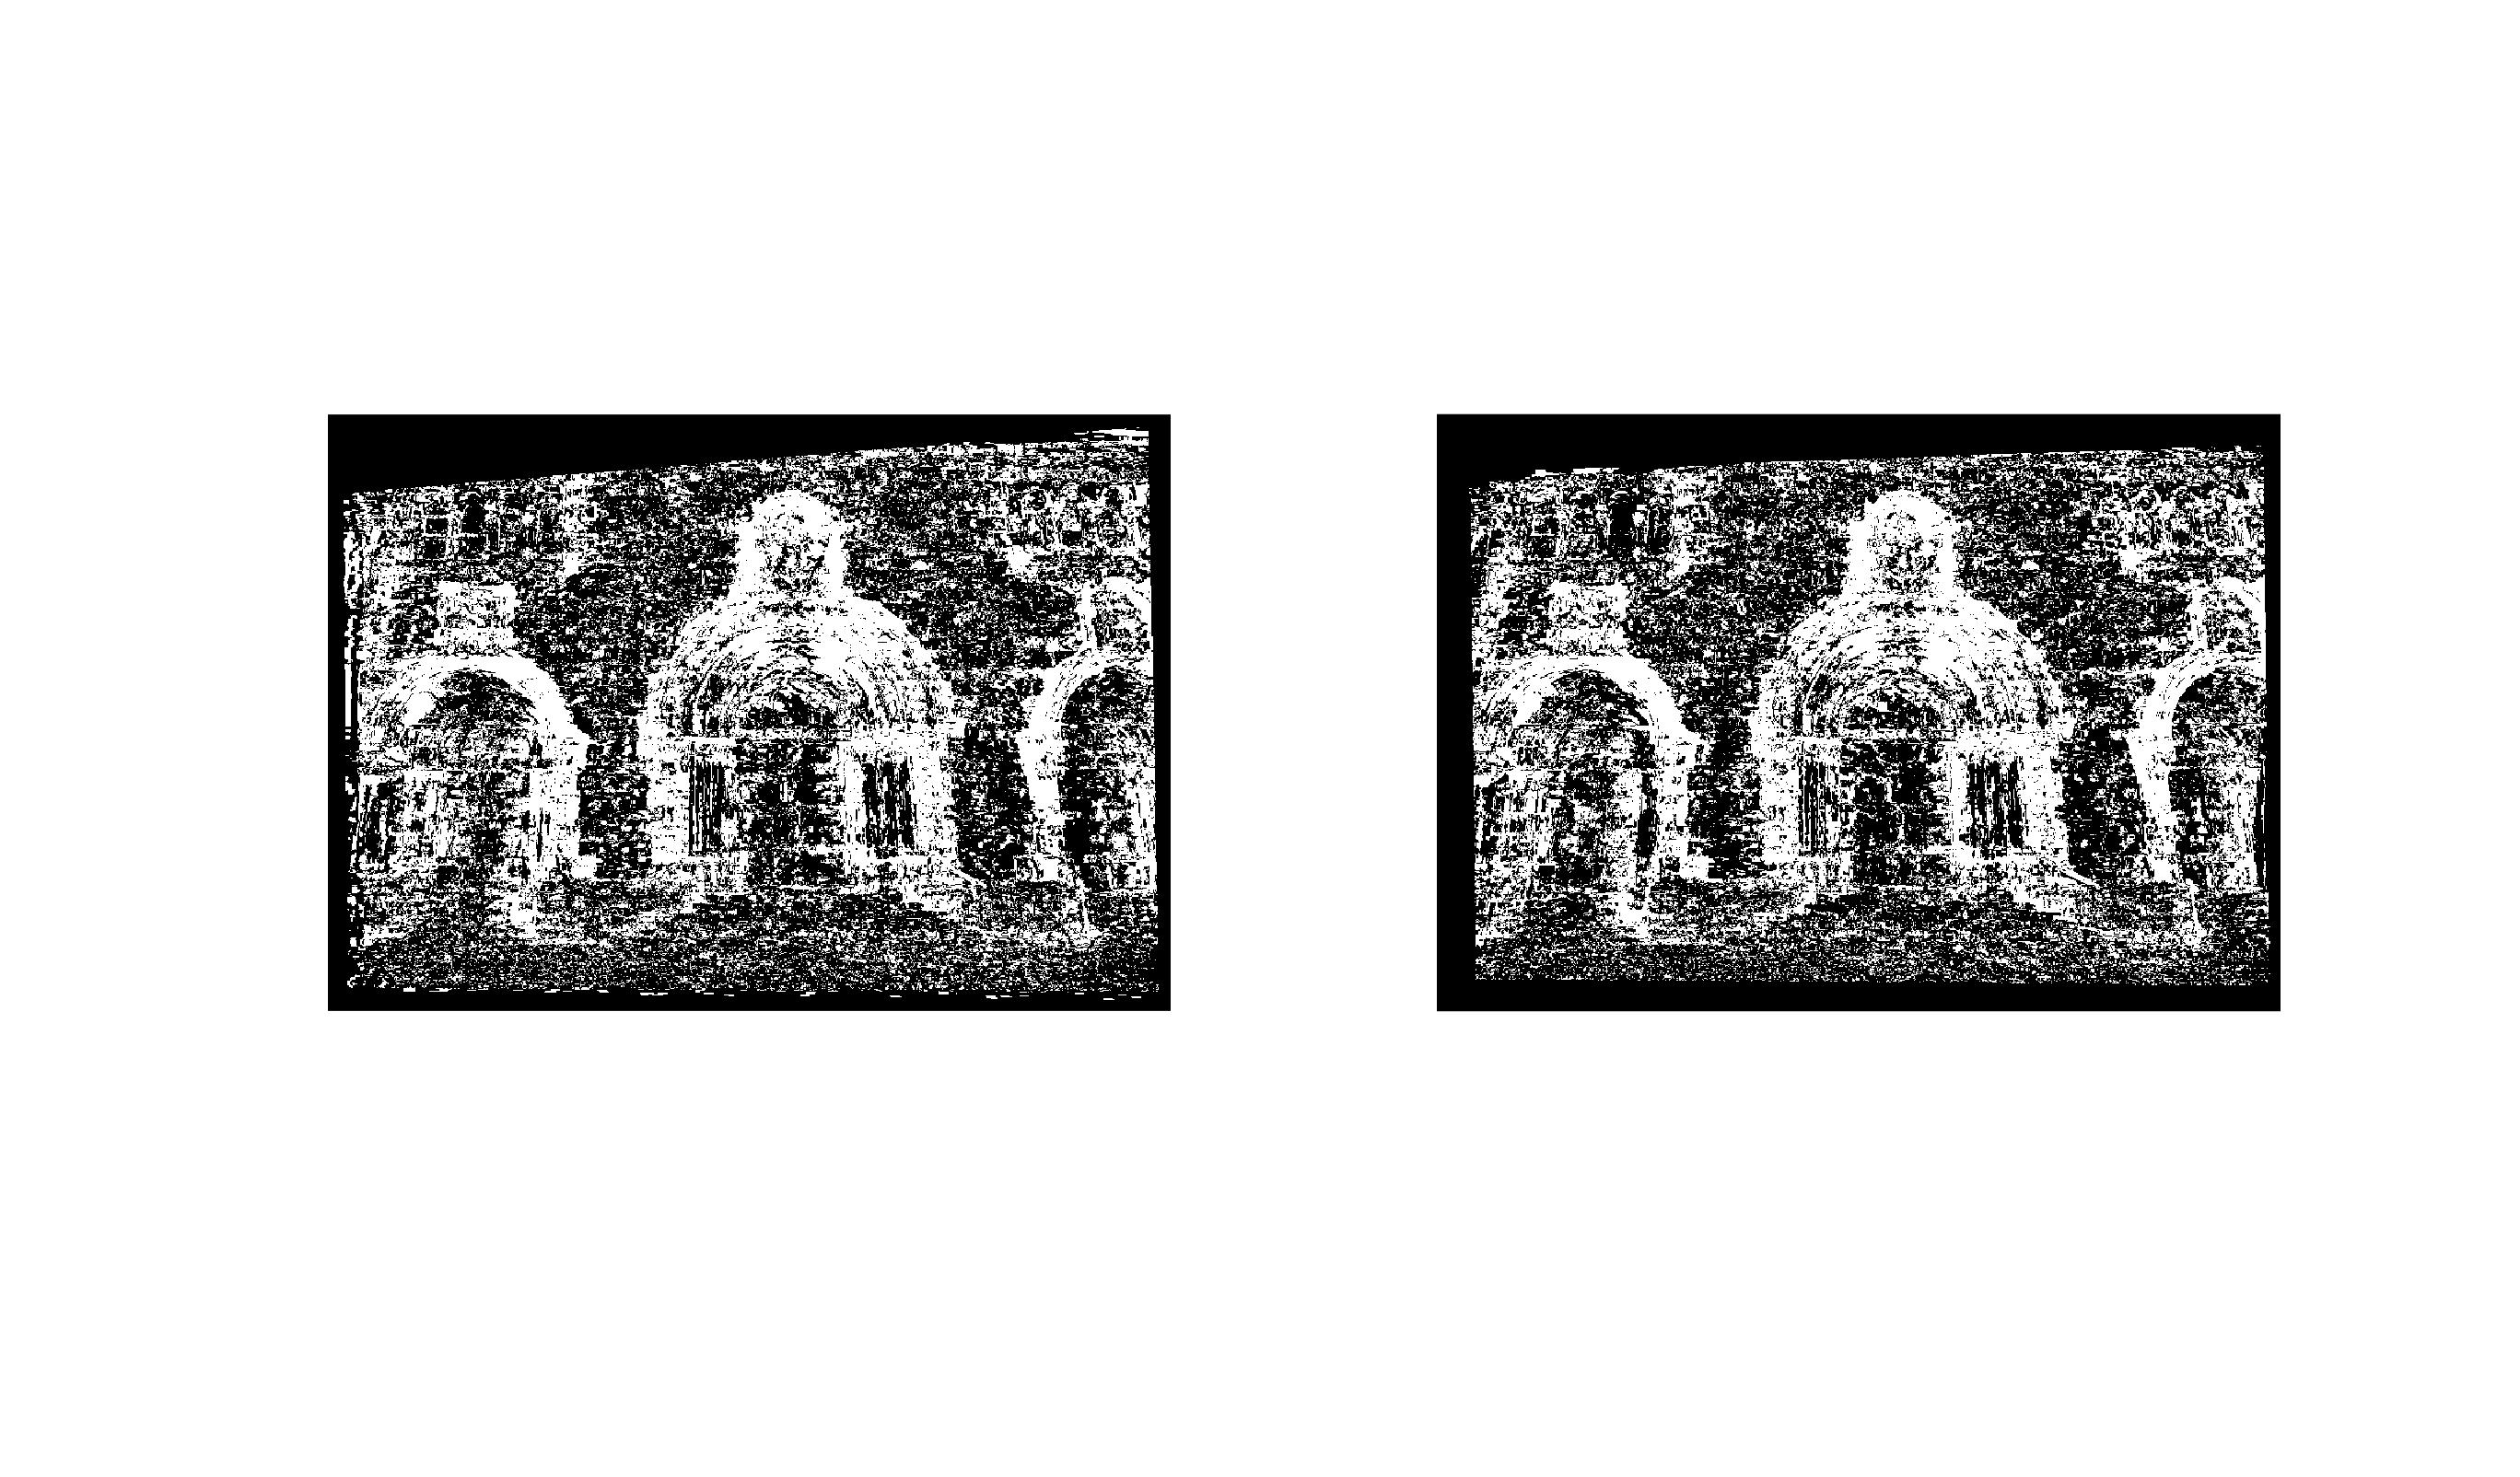
\includegraphics[width=1.1\textwidth]{dc3_2.jpg}
	\caption{3x3 Filter Window}
	\label{fig1}
\end{figure}
\vspace{5mm}
\begin{figure}[H]
	\centering
	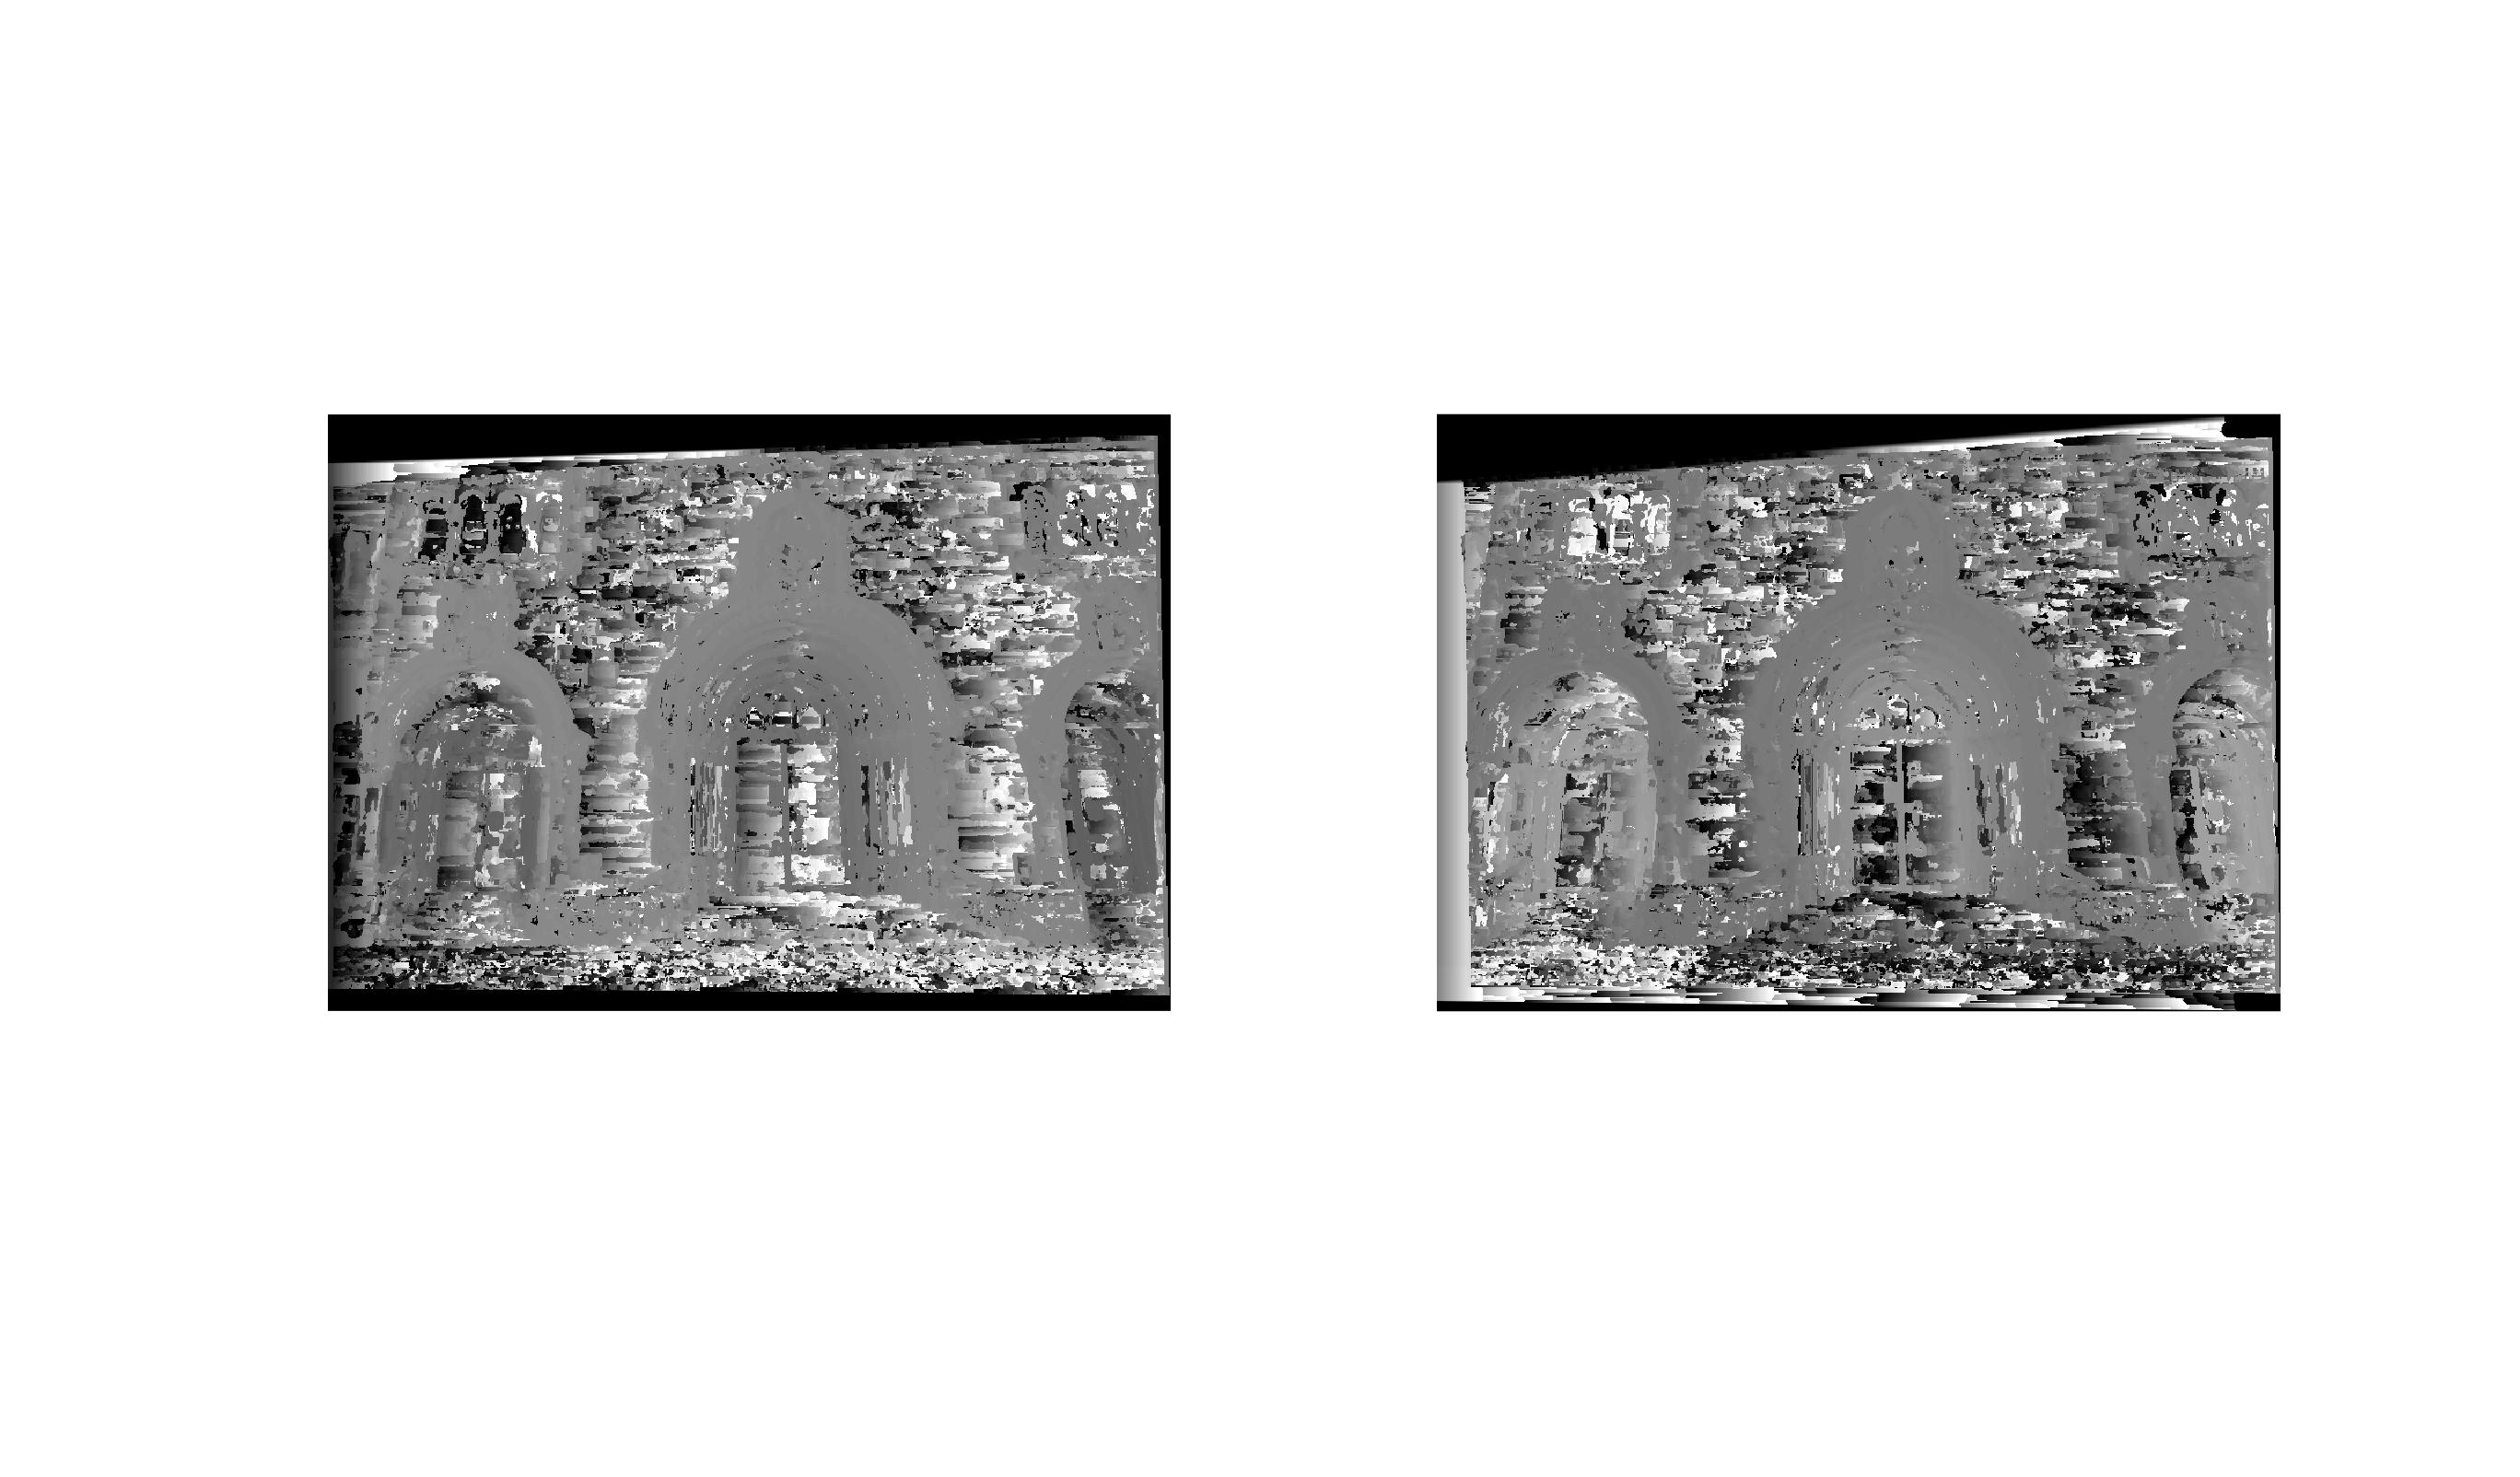
\includegraphics[width=1.1\textwidth]{dc5_1.jpg}
	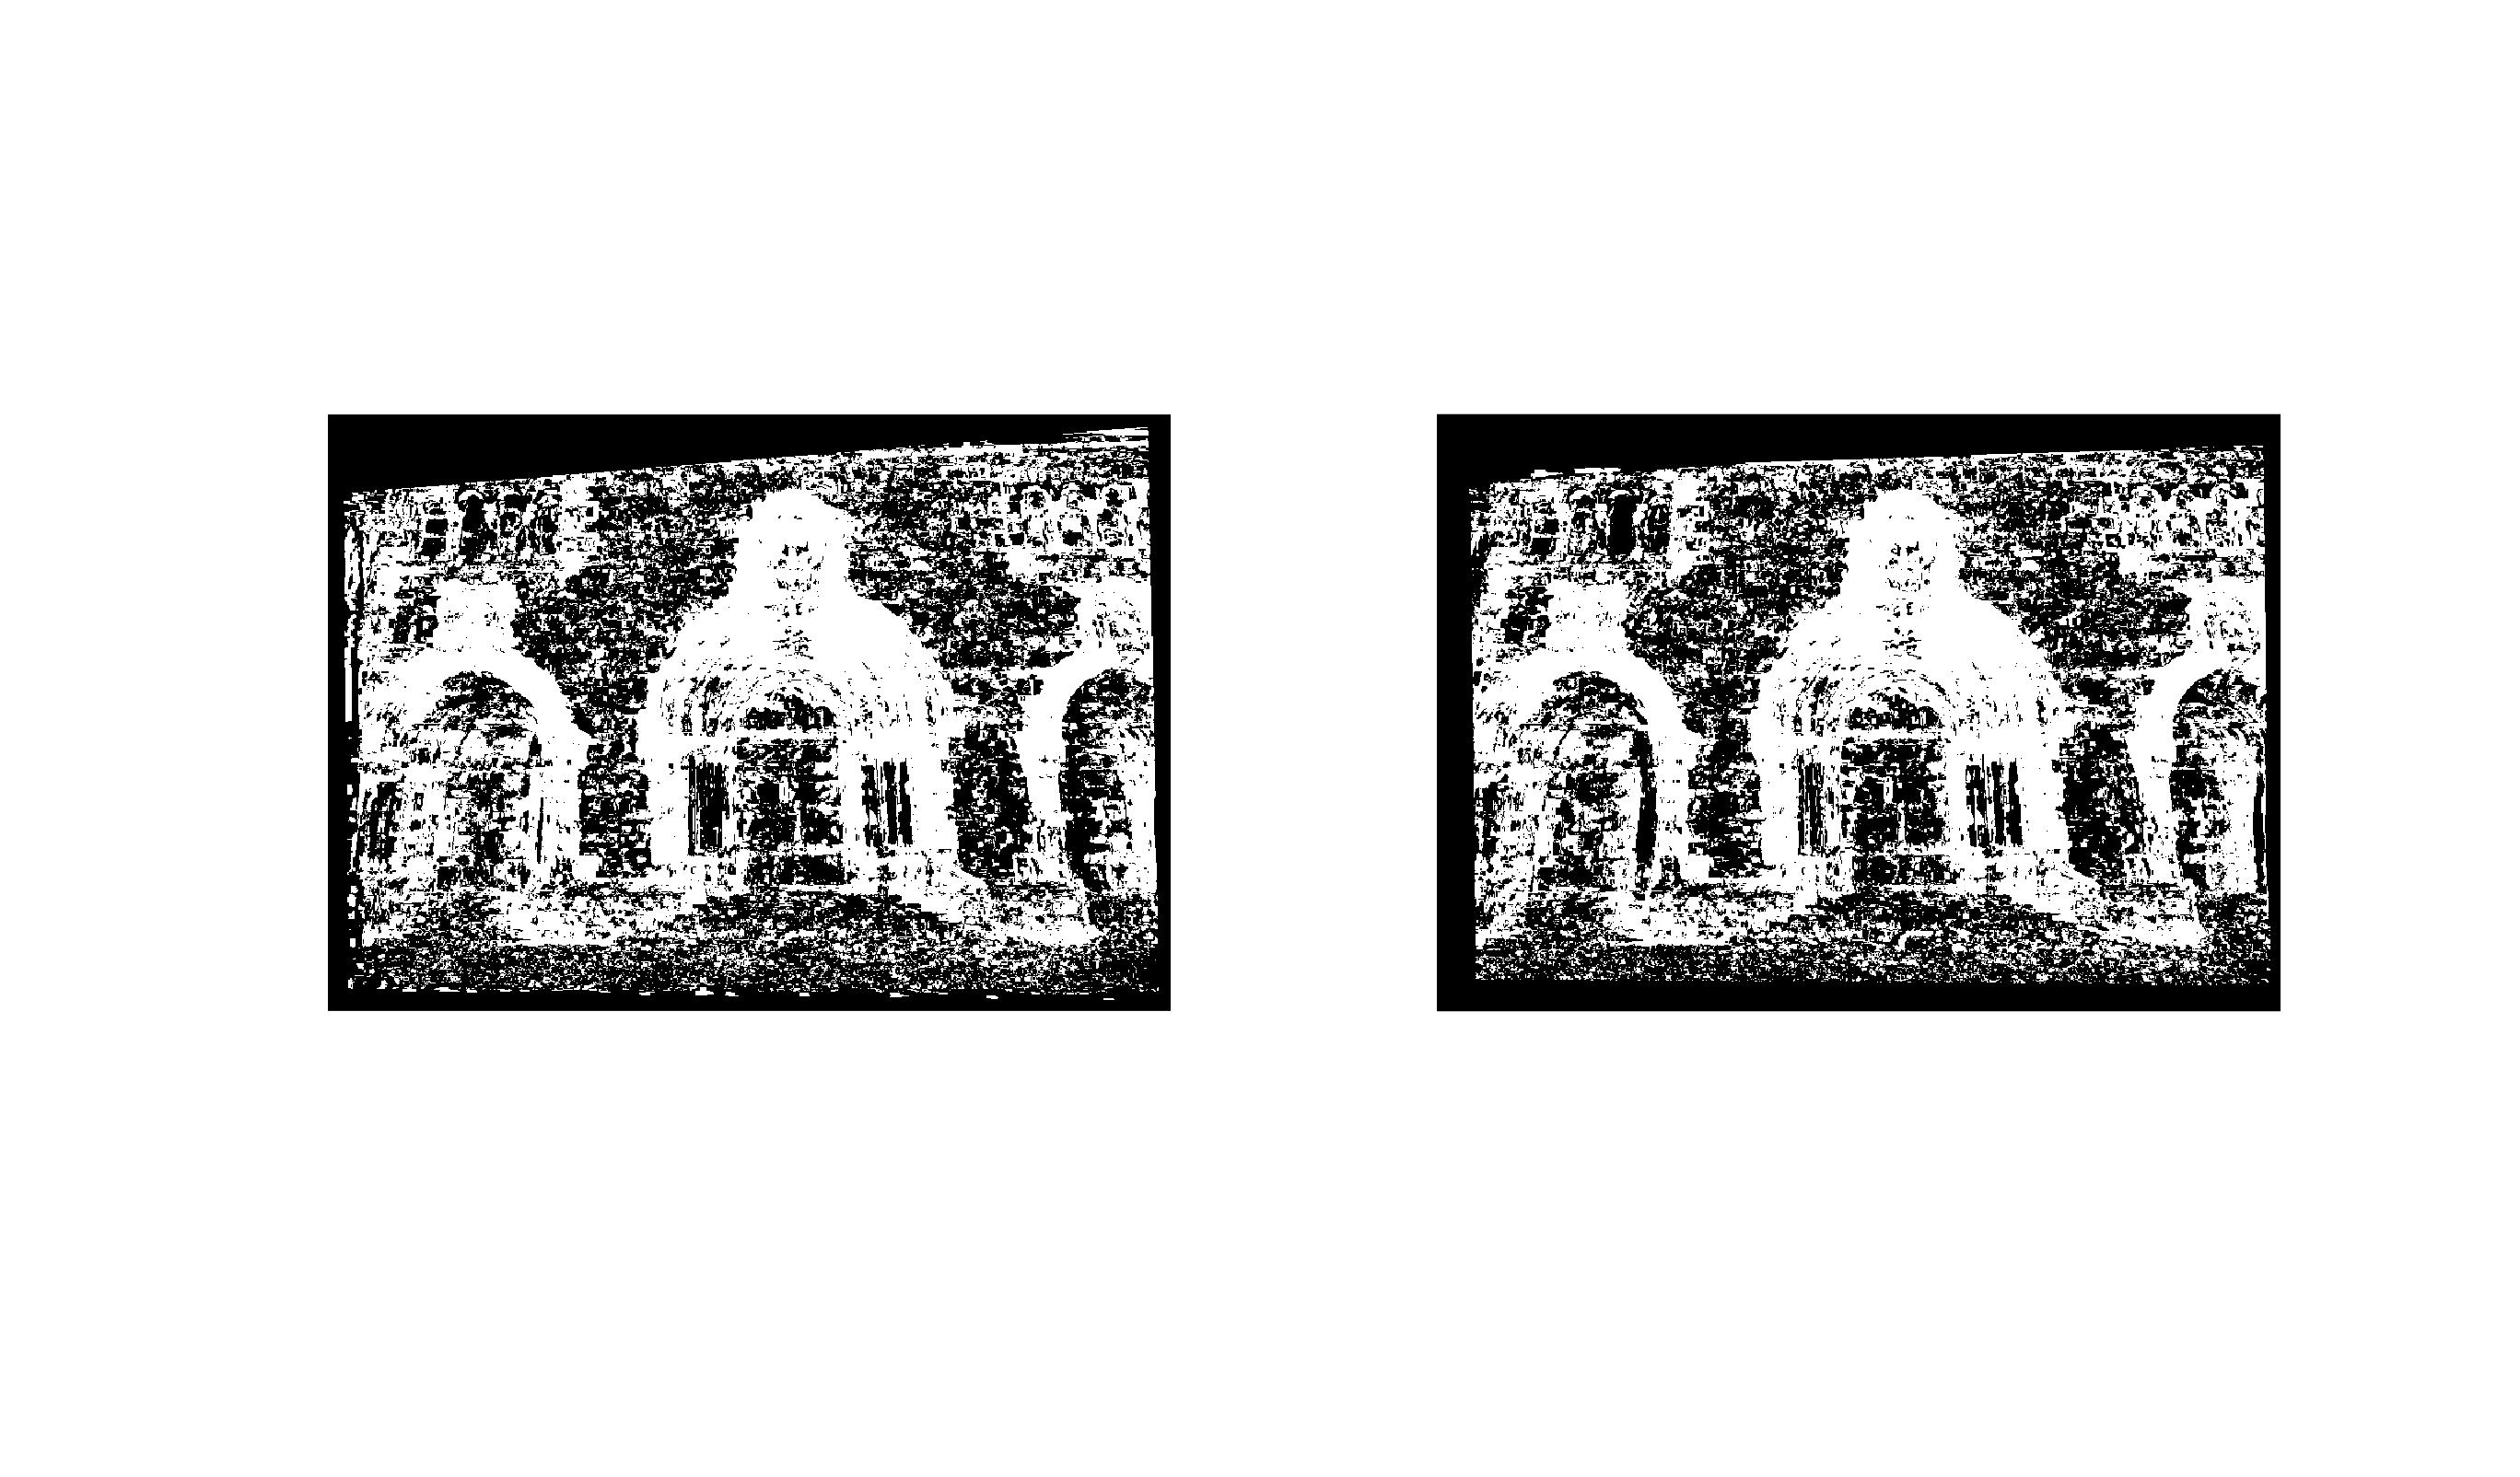
\includegraphics[width=1.1\textwidth]{dc5_2.jpg}
	\caption{5x5 Filter Window}
	\label{fig1}
\end{figure}
\vspace{5mm}
\begin{figure}[H]
	\centering
	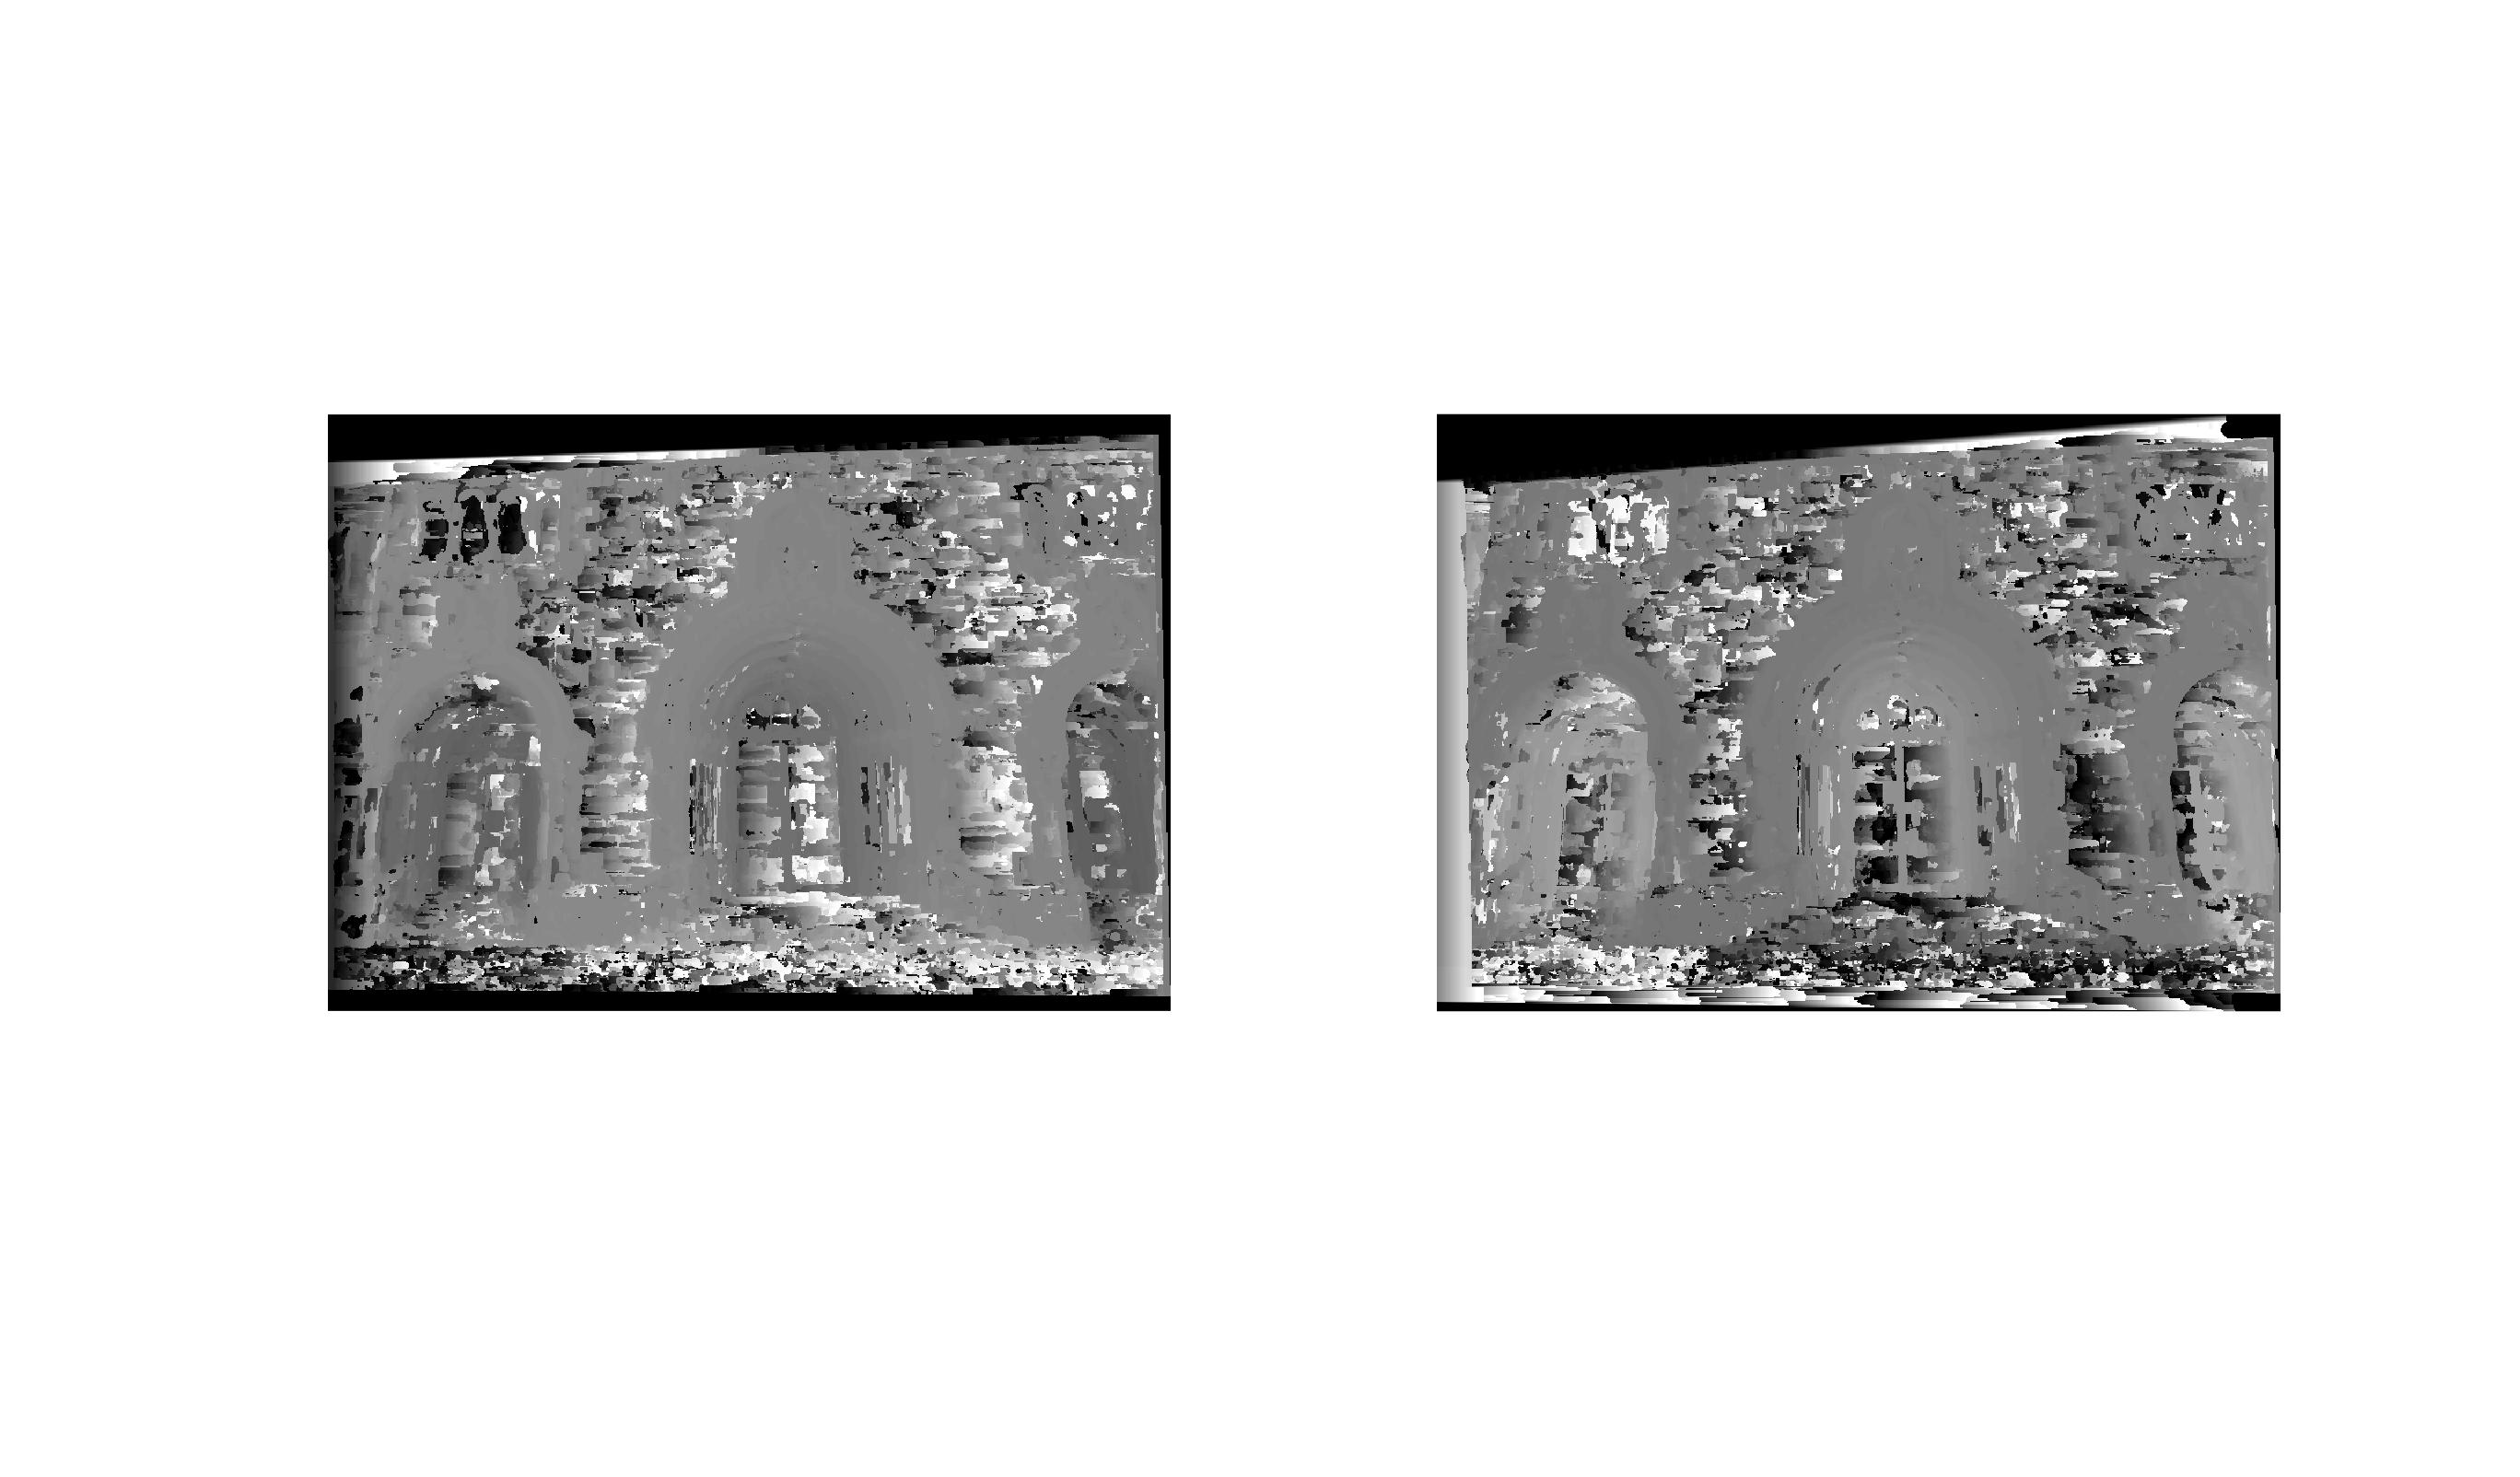
\includegraphics[width=1.1\textwidth]{dc7_1.jpg}
	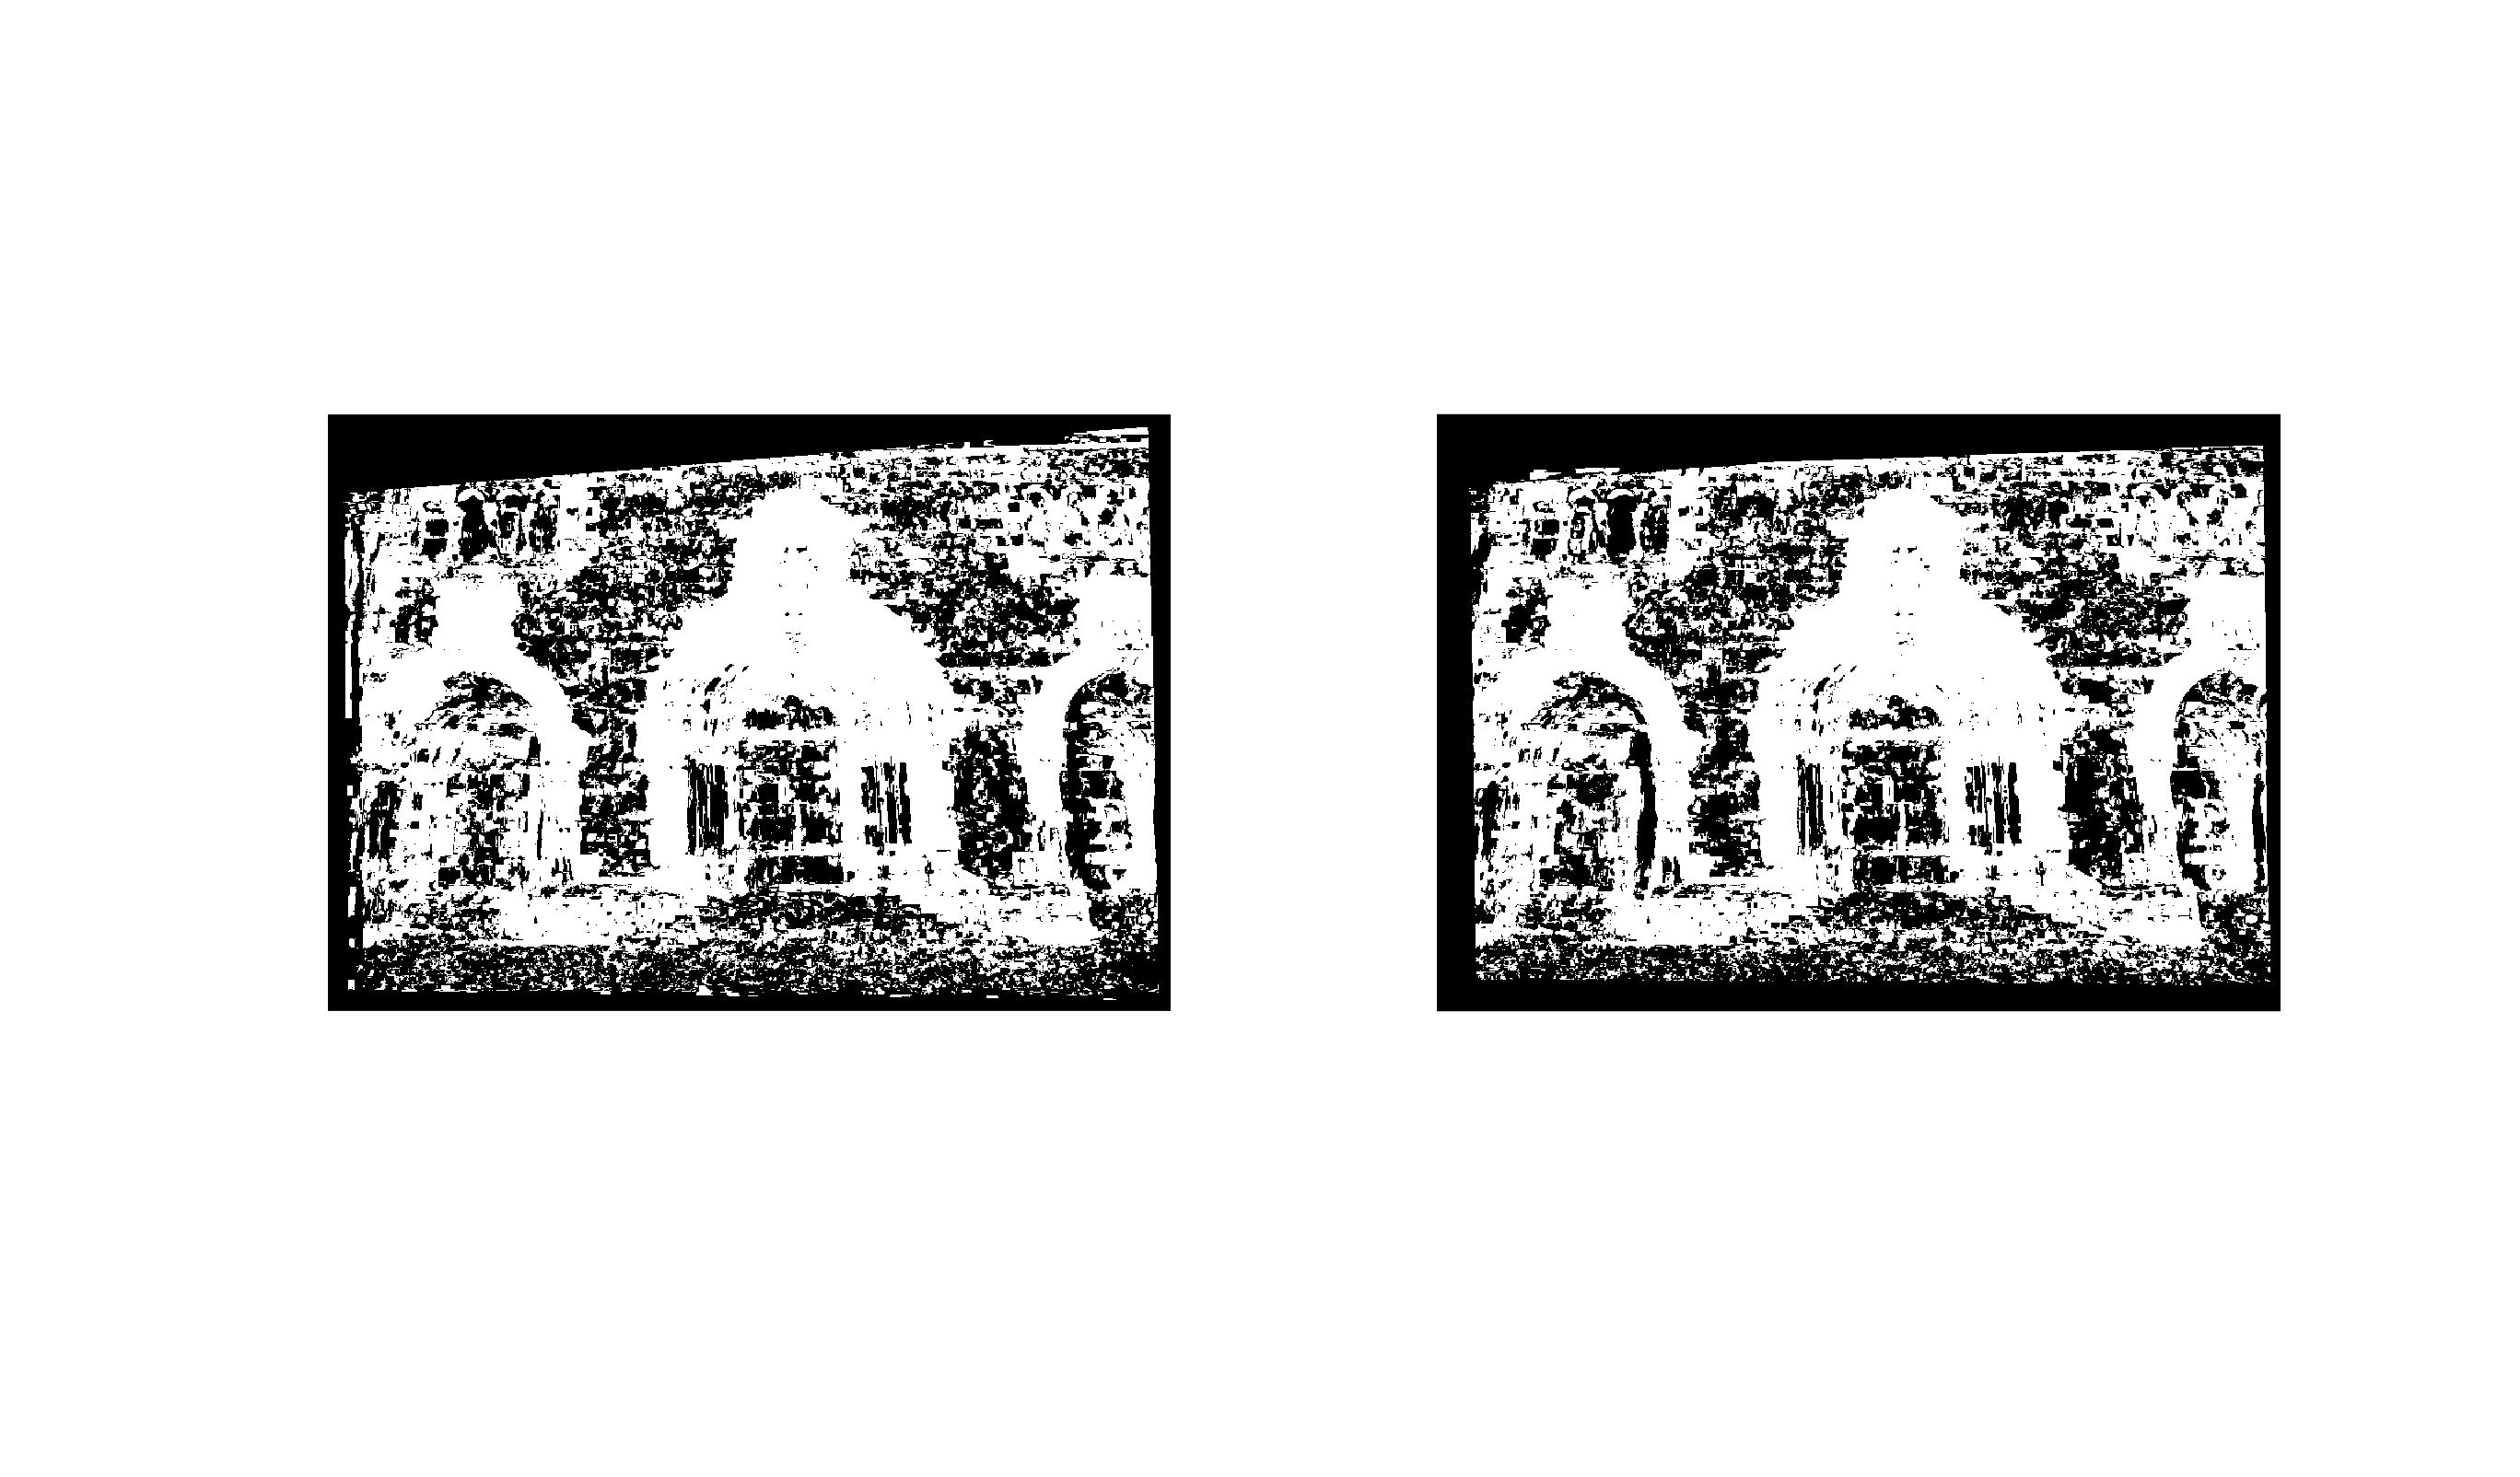
\includegraphics[width=1.1\textwidth]{dc7_2.jpg}
	\caption{7x7 Filter Window}
	\label{fig1}
\end{figure}
\vspace{5mm}
\begin{figure}[H]
	\centering
	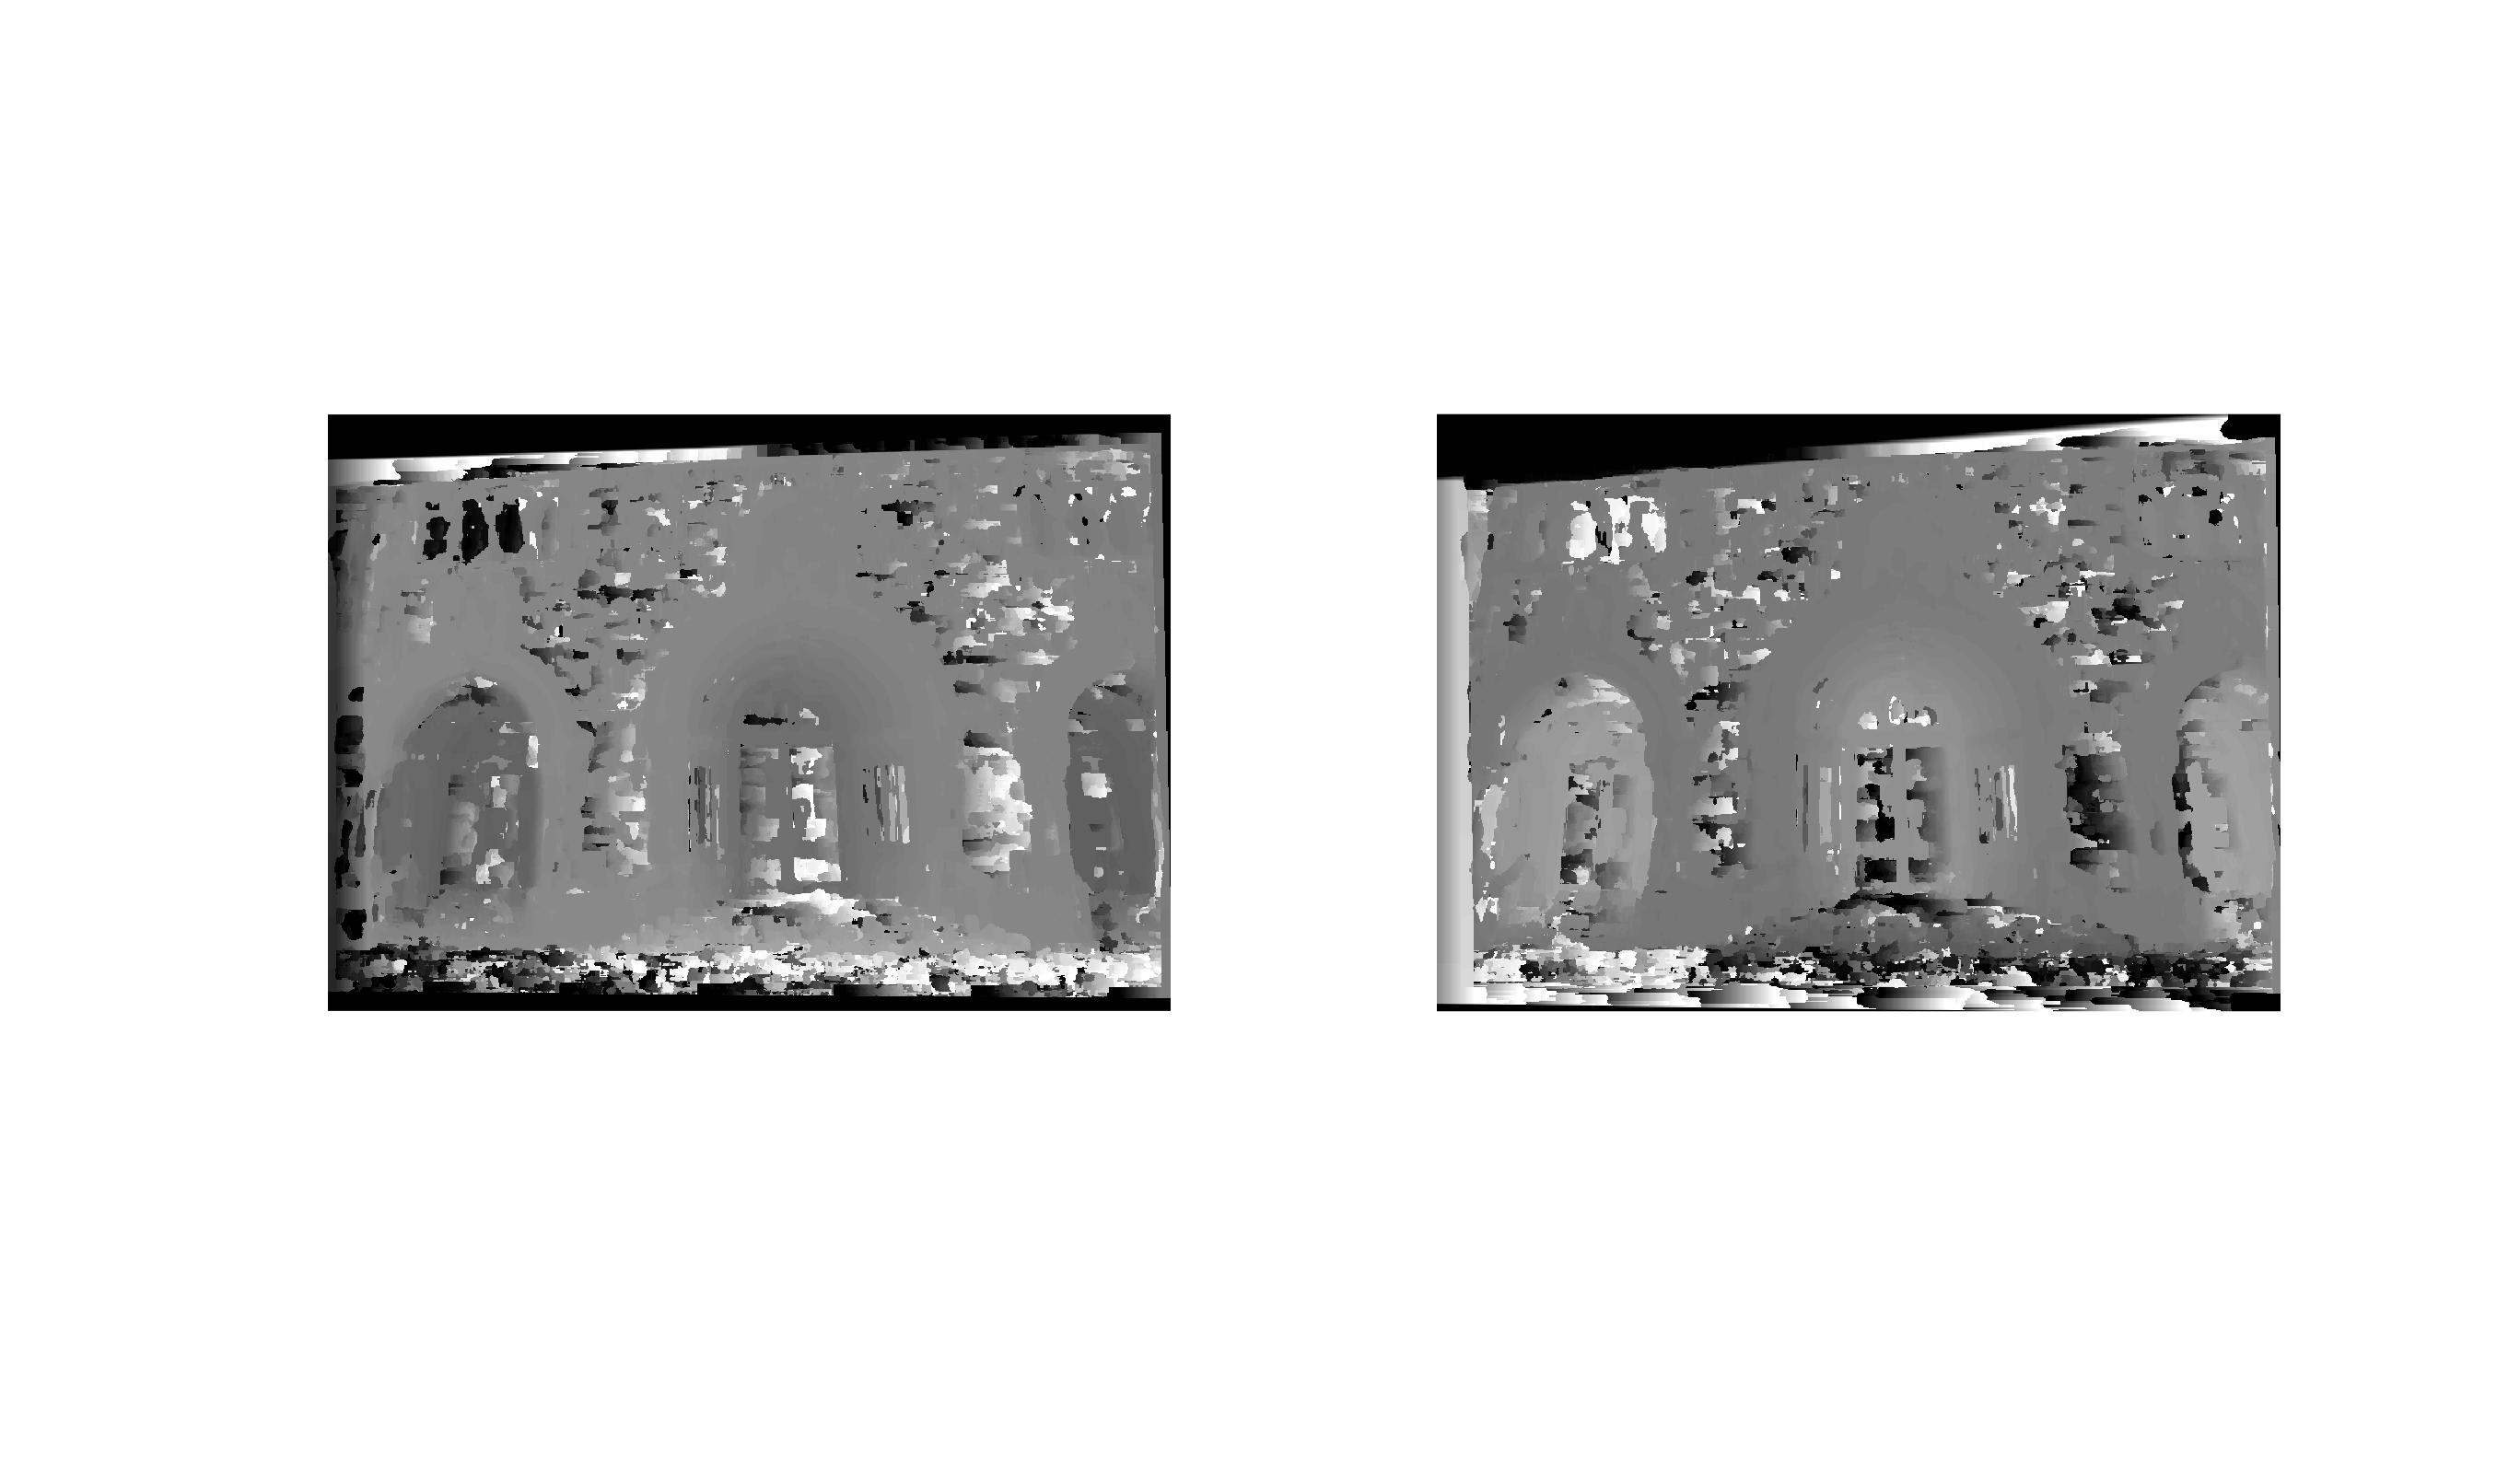
\includegraphics[width=1.1\textwidth]{dc11_1.jpg}
	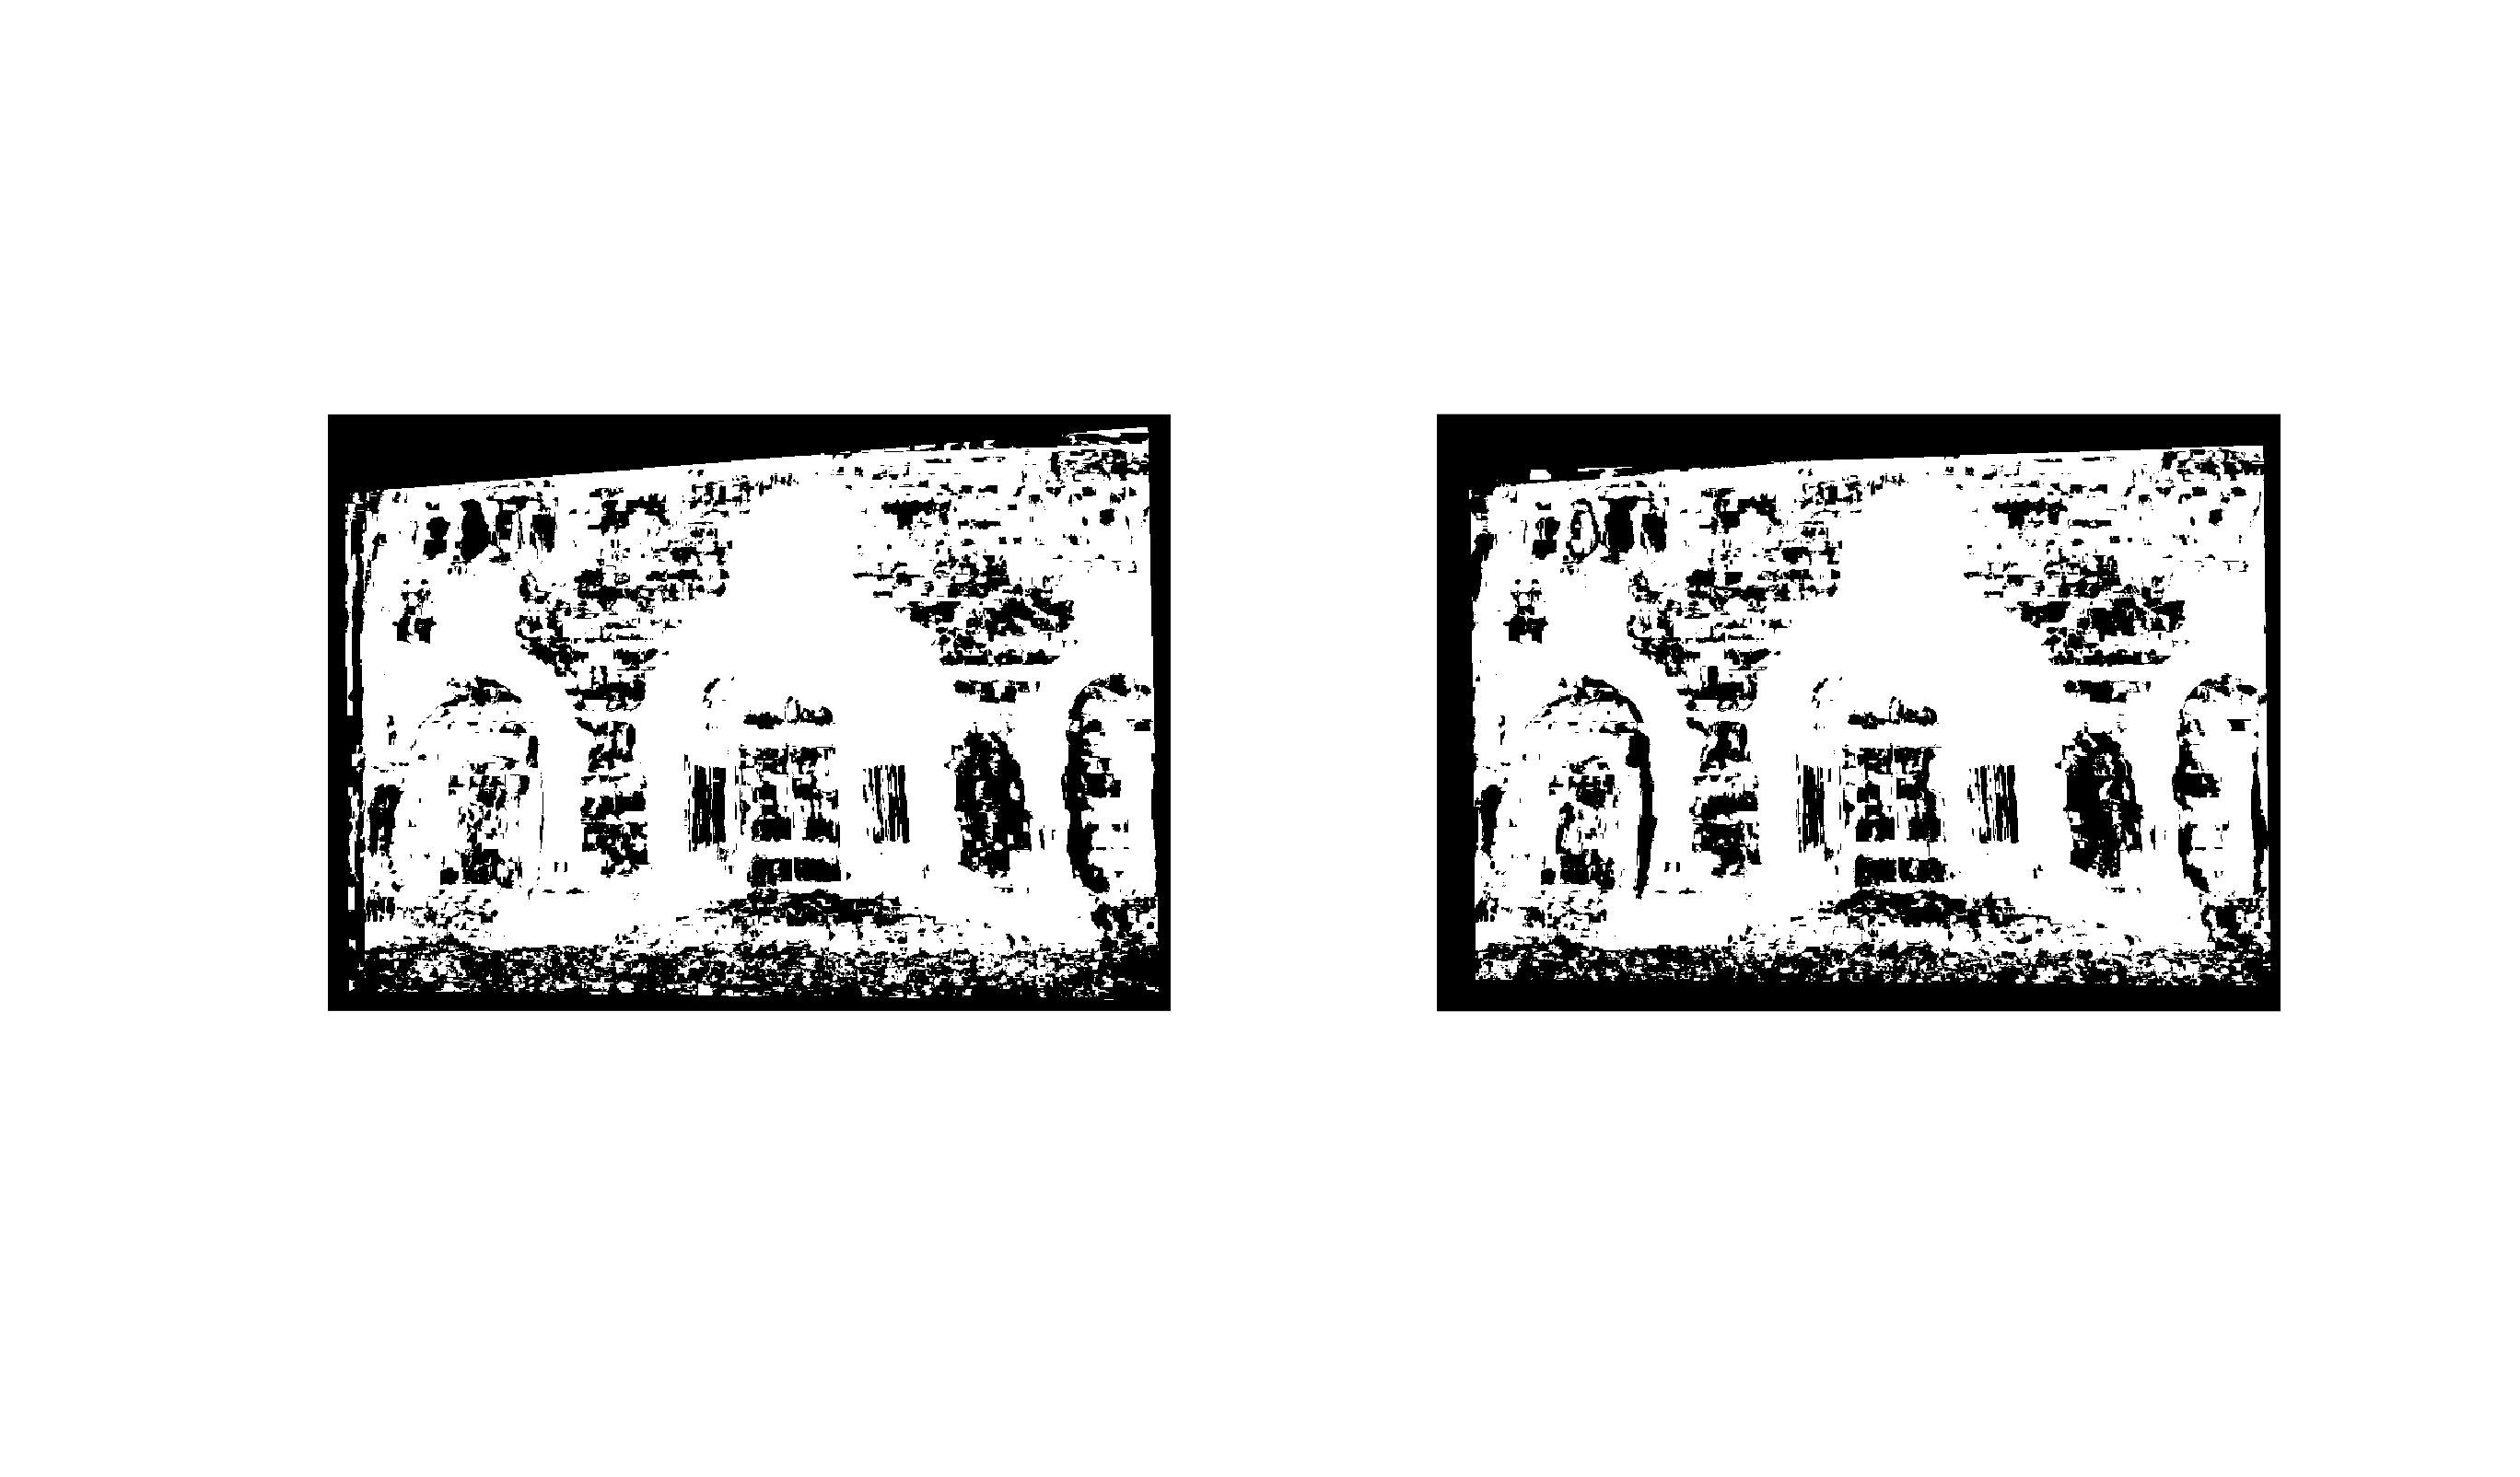
\includegraphics[width=1.1\textwidth]{dc11_2.jpg}
	\caption{11x11 Filter Window}
	\label{fig1}
\end{figure}
\vspace{5mm}
\begin{figure}[H]
	\centering
	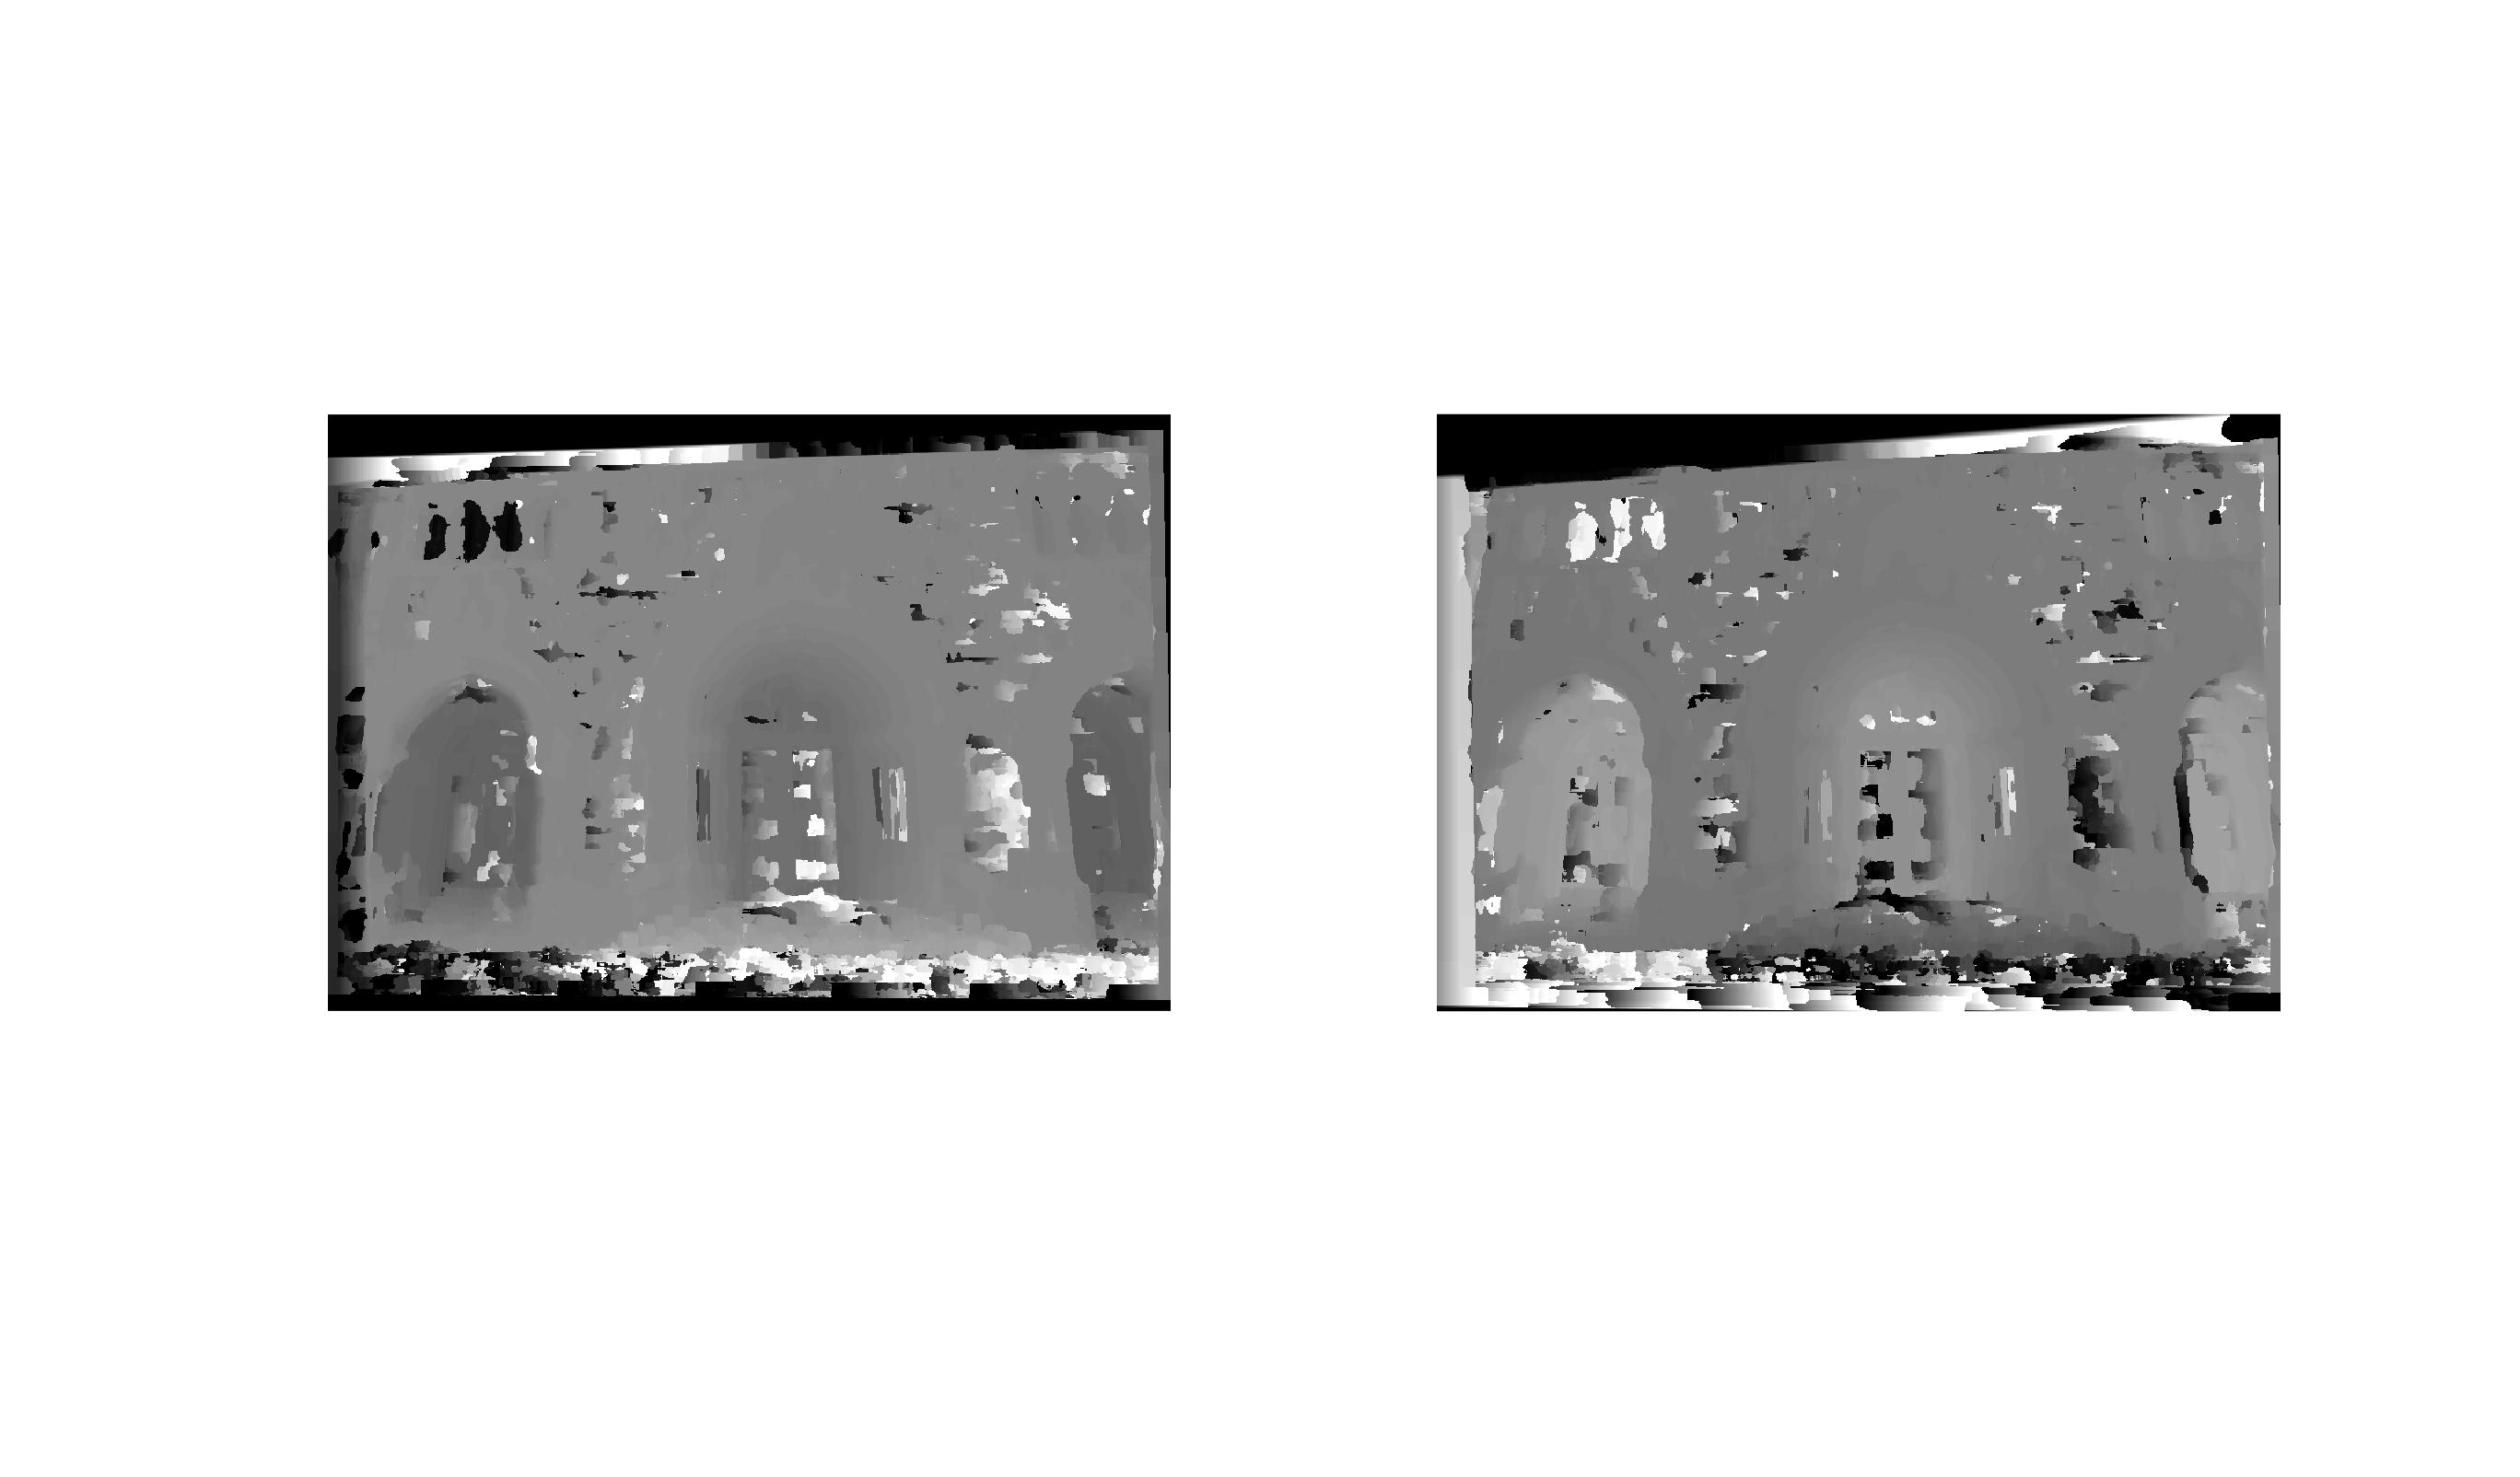
\includegraphics[width=1.1\textwidth]{dc15_1.jpg}
	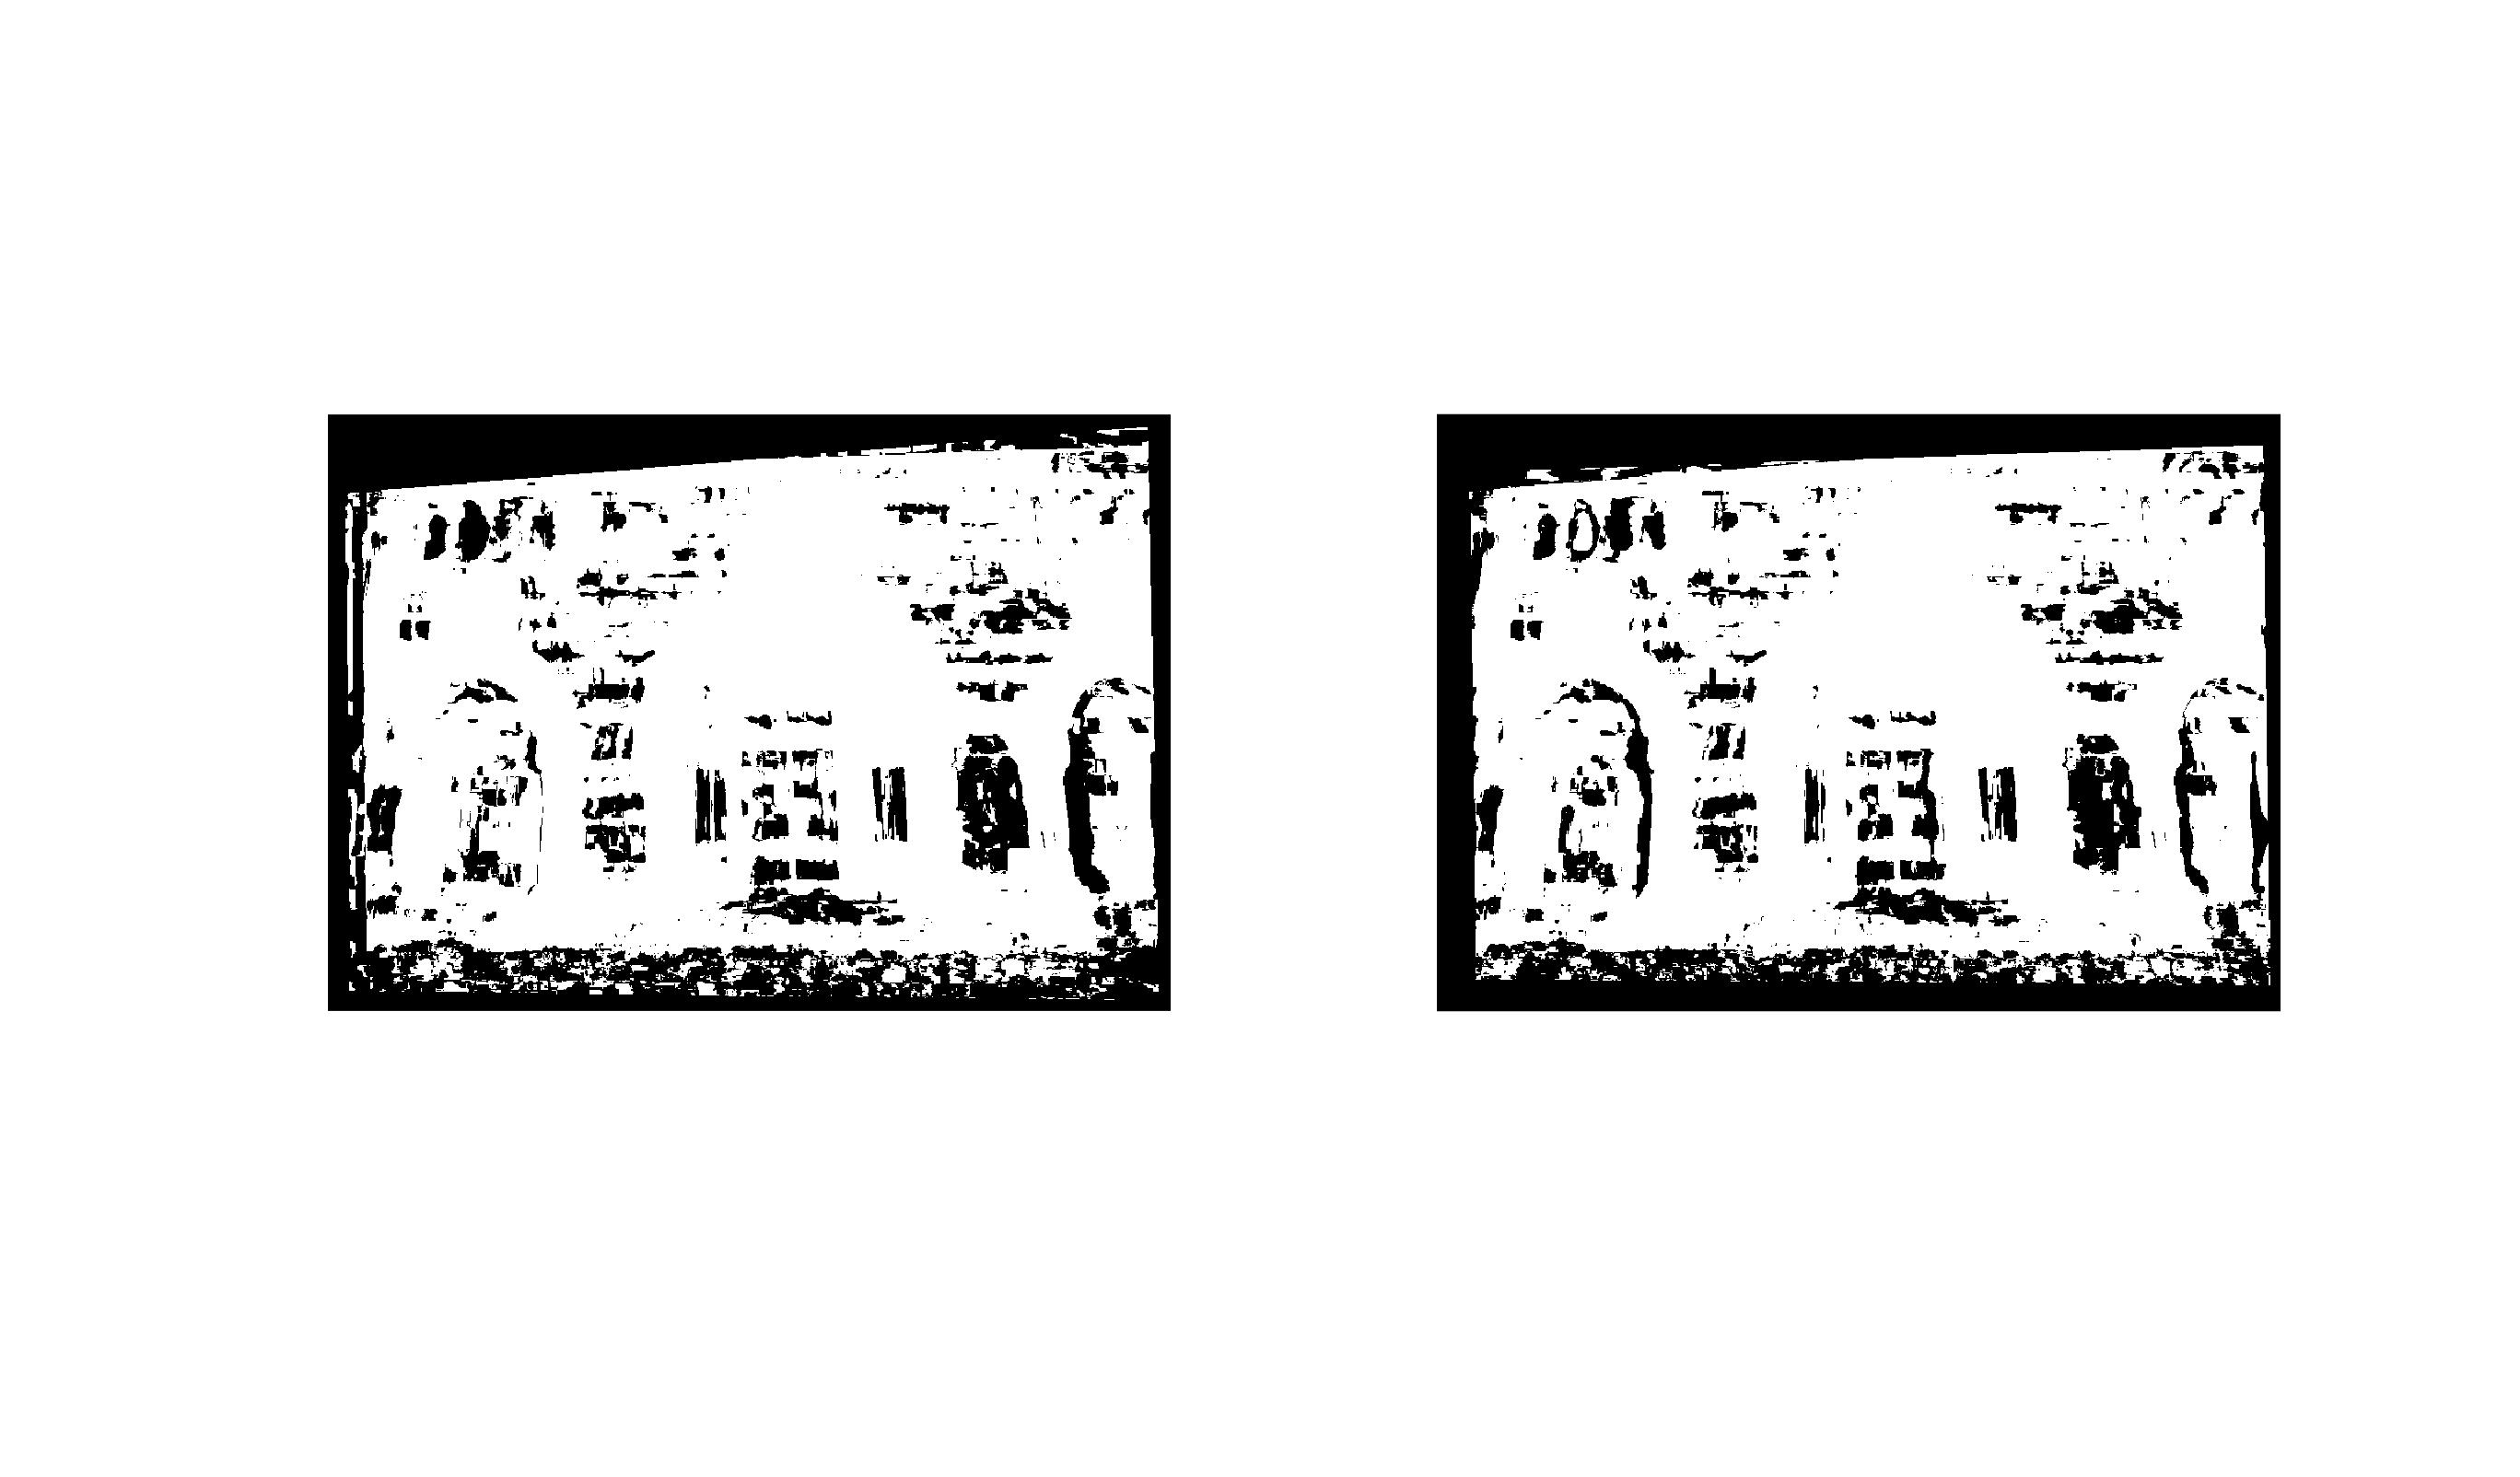
\includegraphics[width=1.1\textwidth]{dc15_2.jpg}
	\caption{15x15 Filter Window}
	\label{fig1}
\end{figure}
\vspace{5mm}
\begin{figure}[H]
	\centering
	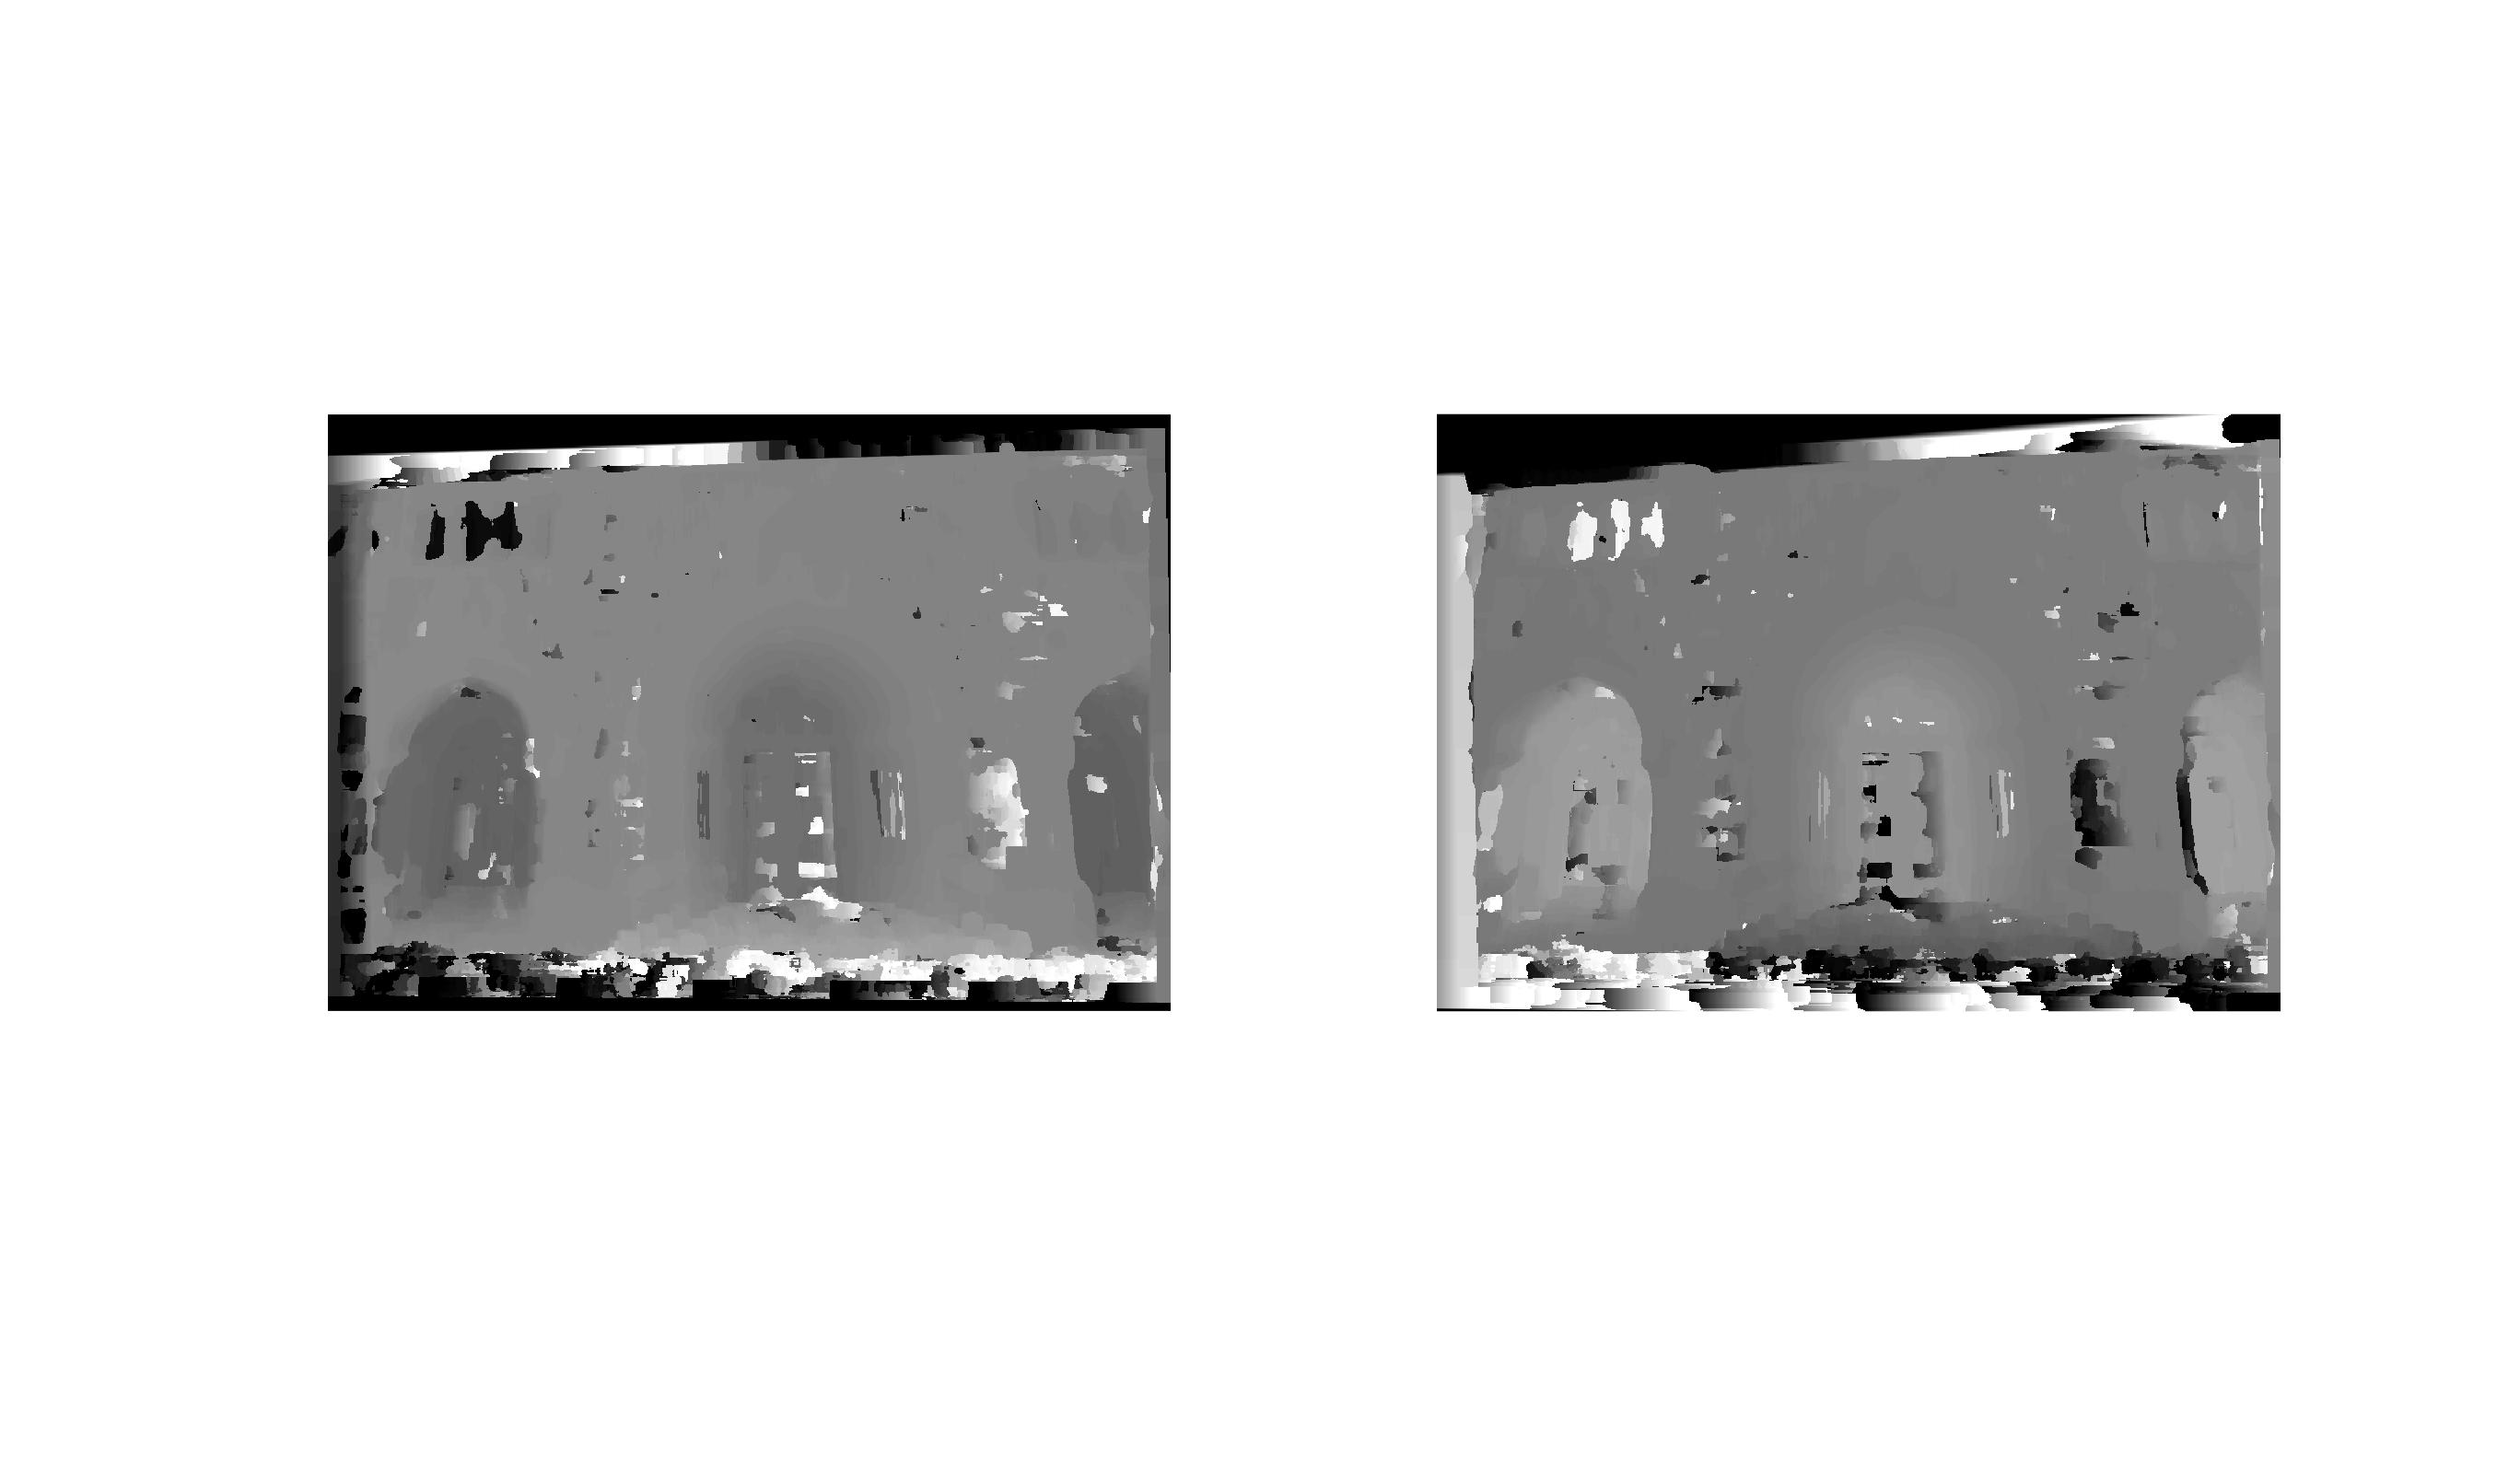
\includegraphics[width=1.1\textwidth]{dc19_1.jpg}
	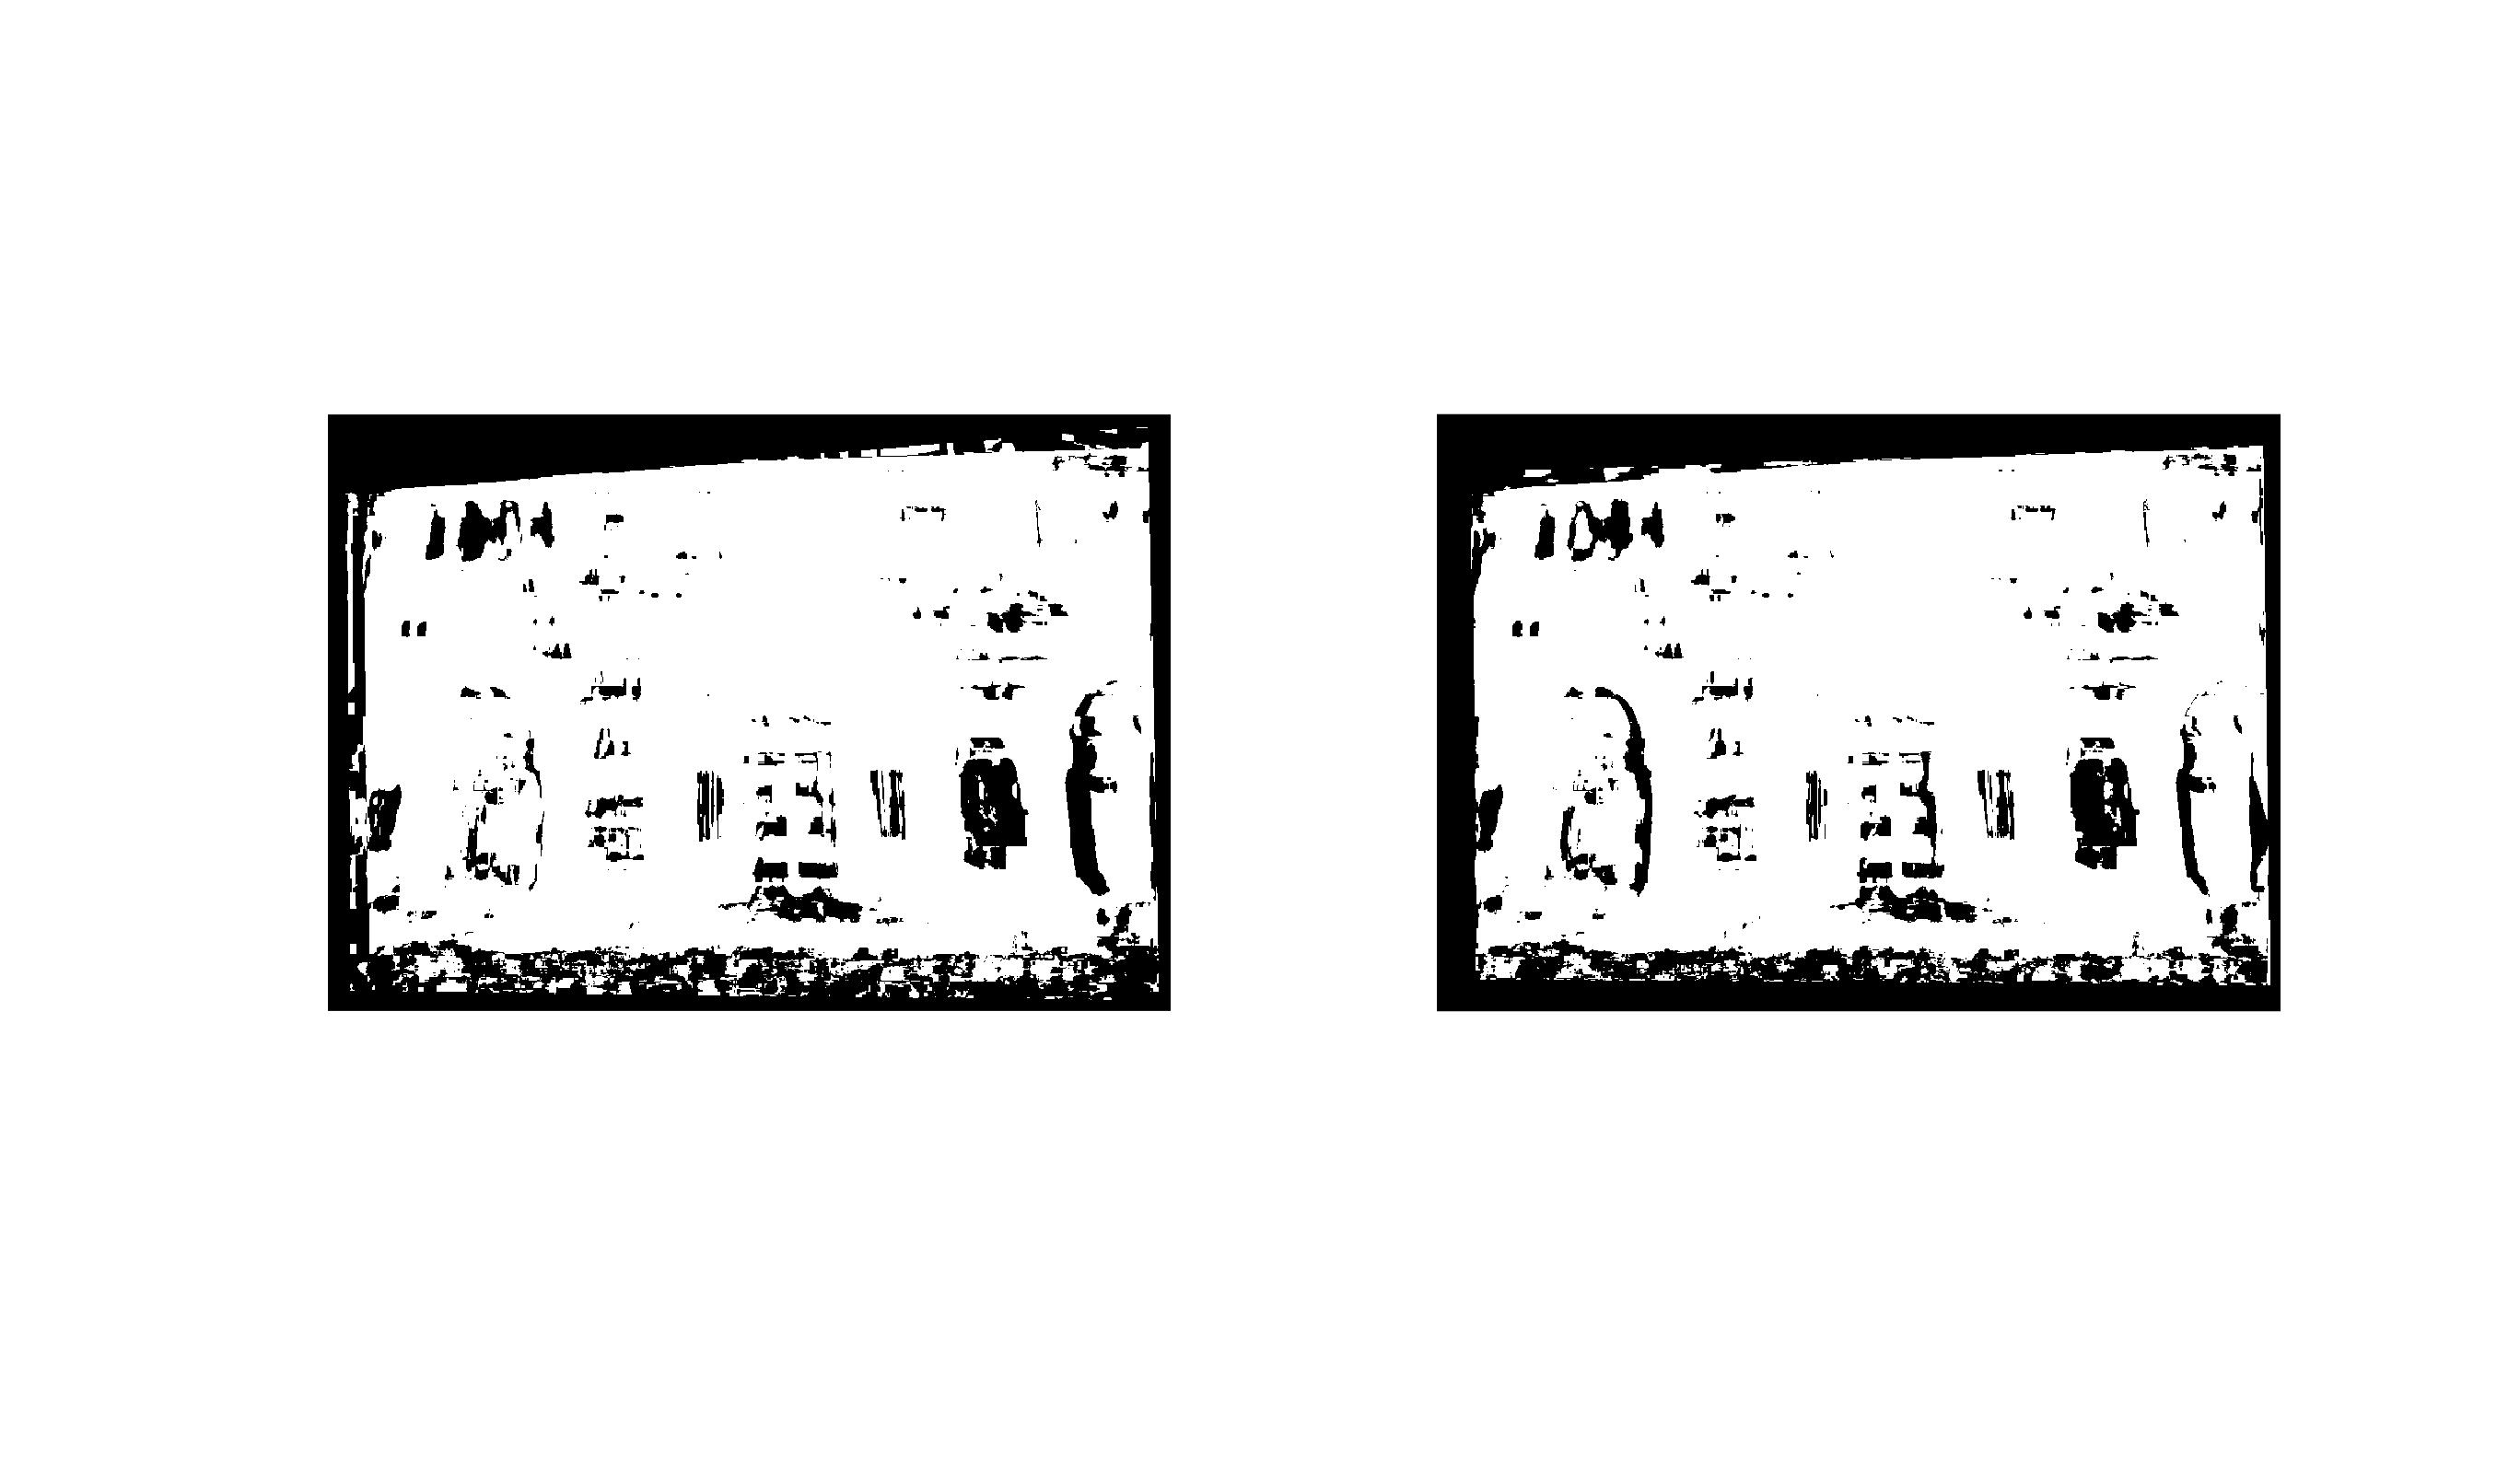
\includegraphics[width=1.1\textwidth]{dc19_2.jpg}
	\caption{19x19 Filter Window}
	\label{fig1}
\end{figure}
\vspace{5mm}

By looking at the black and white pictures the points which are correctly maped (in white) according to the given function can be seen. As the filter window is increased the disparity map gets less sensitive to noise, which makes intuitive sense. As can be seen, especially arounfd edges of the stairs and the half circle elements above the door some details can be lost snd edges get smoothed out. So depending on the application a tradeoff value has to be found here.
\newline
Furthermore, it can be seen that the algorithm performs especially poorely on the flat stone brick surface. Since the stonebricks are arranged in a pattern this might lead to some wrong distance matches (especially between stone block edges) with the given range. Without adjusting the range this can only be fixed by extensive filtering.  

\begin{figure}[H]
	\centering
	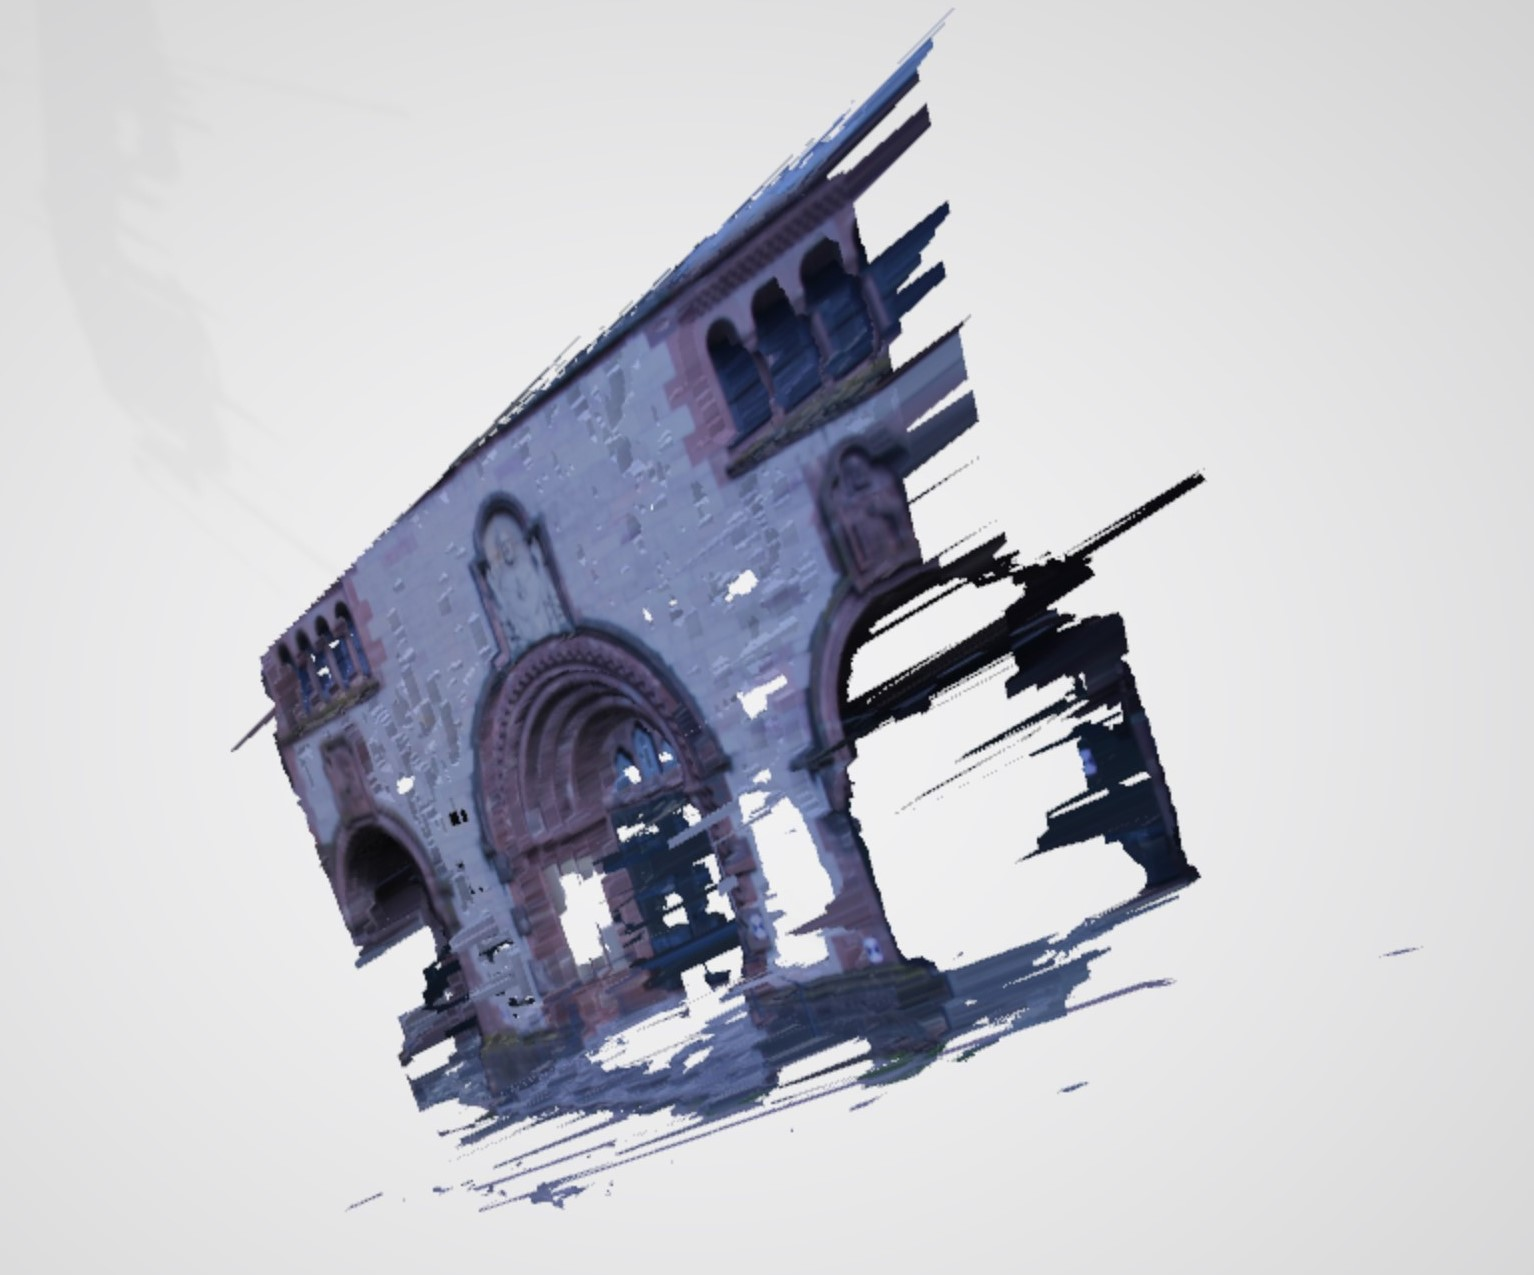
\includegraphics[width=0.6\textwidth]{dc_model_19.jpg}
	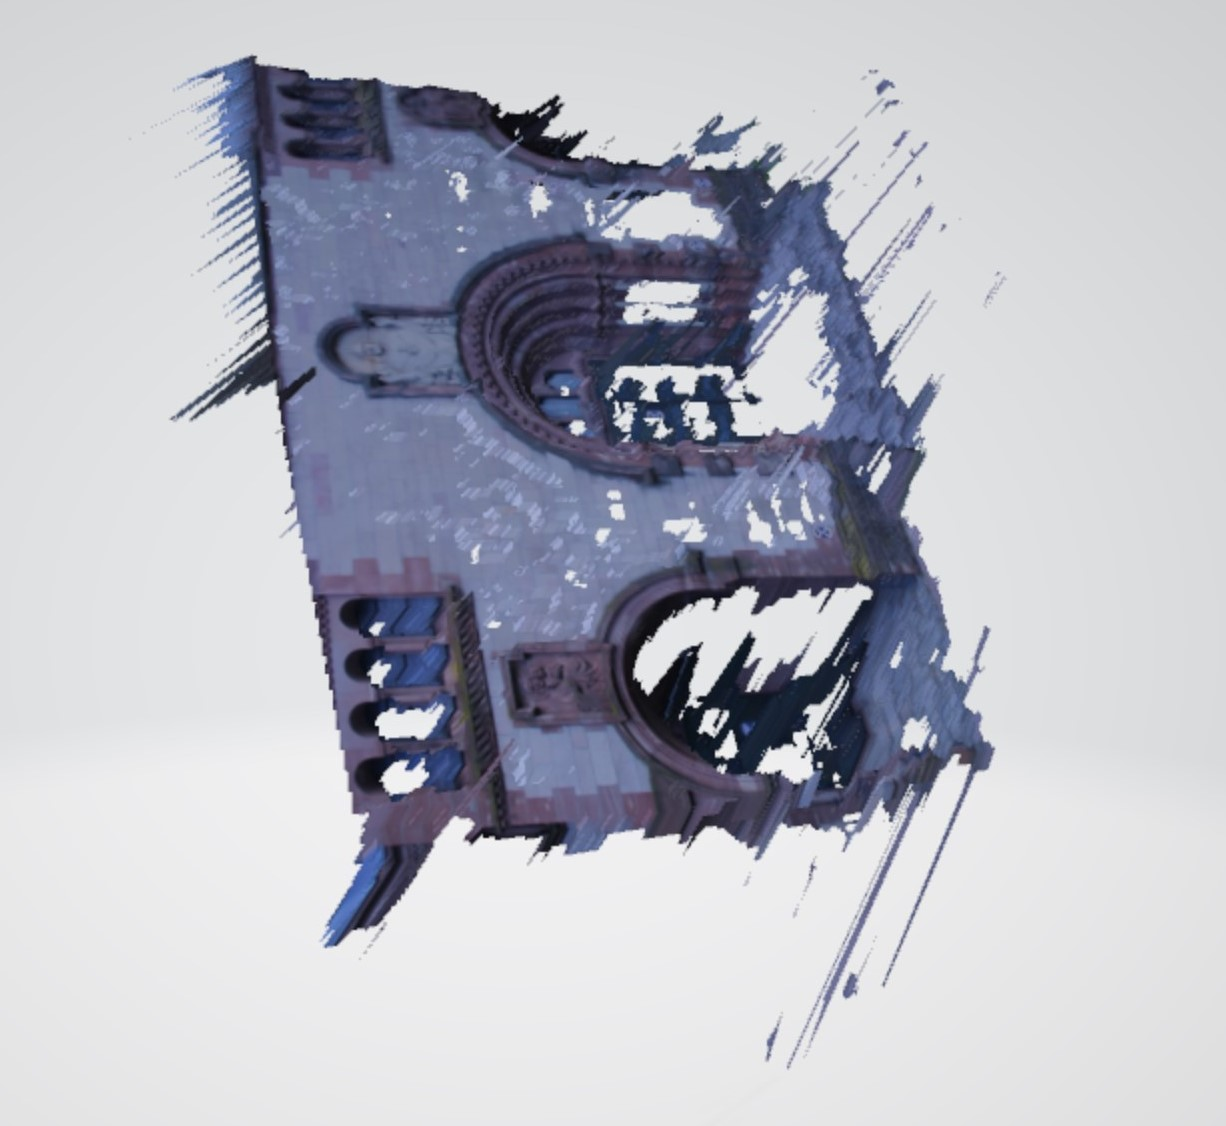
\includegraphics[width=0.6\textwidth]{dc_model_19_2.jpg}
	\caption{Textured 3D Model from Disparity Computation with range $[-40, 40]$ and filter Window Size 19}
	\label{fig1}
\end{figure}

As can be seen in the picture above a somewhat usable 3D reconstruction can already be optained with the right tuning of this algorithm. Doors, stairs and Windows are already visible.  

\section{Graph Cut}

Similar to the exercise before a depth map is obtained by this time using the provided graph cut function. The most important parameters to tune are the filter window size (which was choosen to be 7x7) as well as the scaling of the data cost DC and the smoothness sost SC. Here, Dc is linked to the cost of assigning a label to a pixel of interest and a higher value gives a model with higher accuracy. Sc is linked to assigning labels to the pixels around it and a higher value gives a smoother result.
\vspace{5mm}
\newline
Here are a few of the tried results with variation of DC: 
 
\vspace{5mm}
\begin{figure}[H]
	\centering
	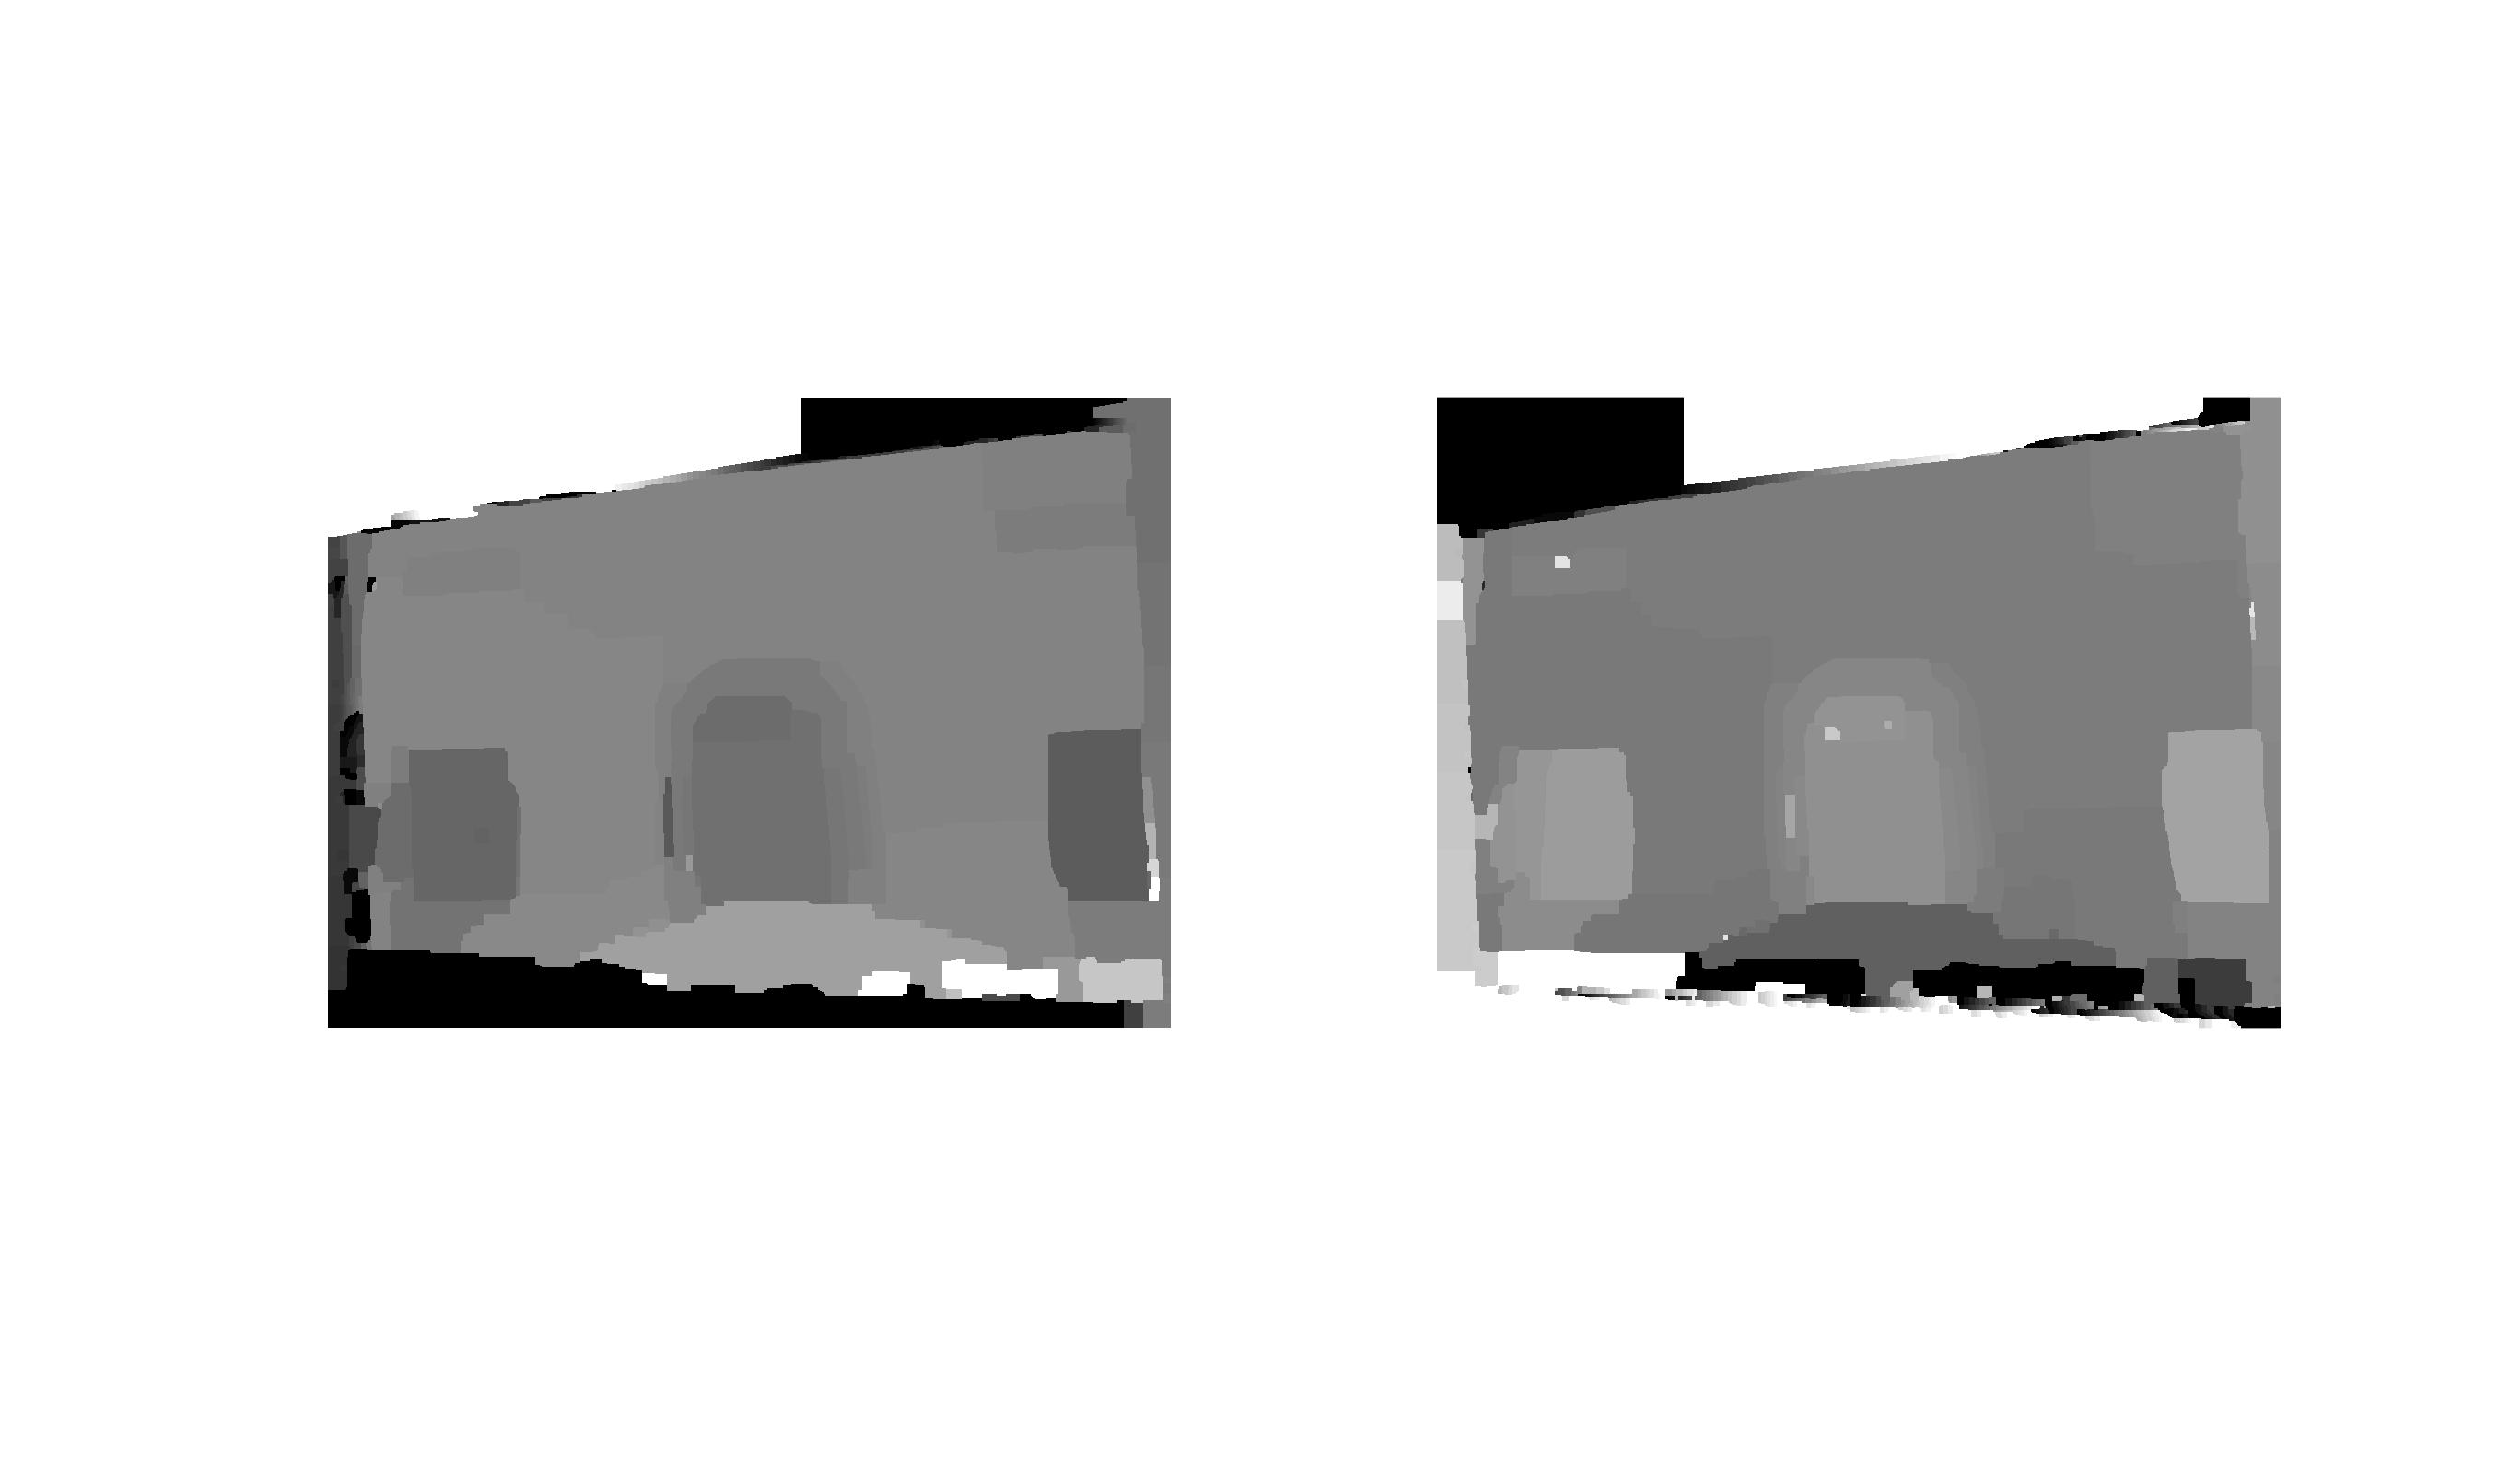
\includegraphics[width=1.1\textwidth]{gc_500_5_1.jpg}
	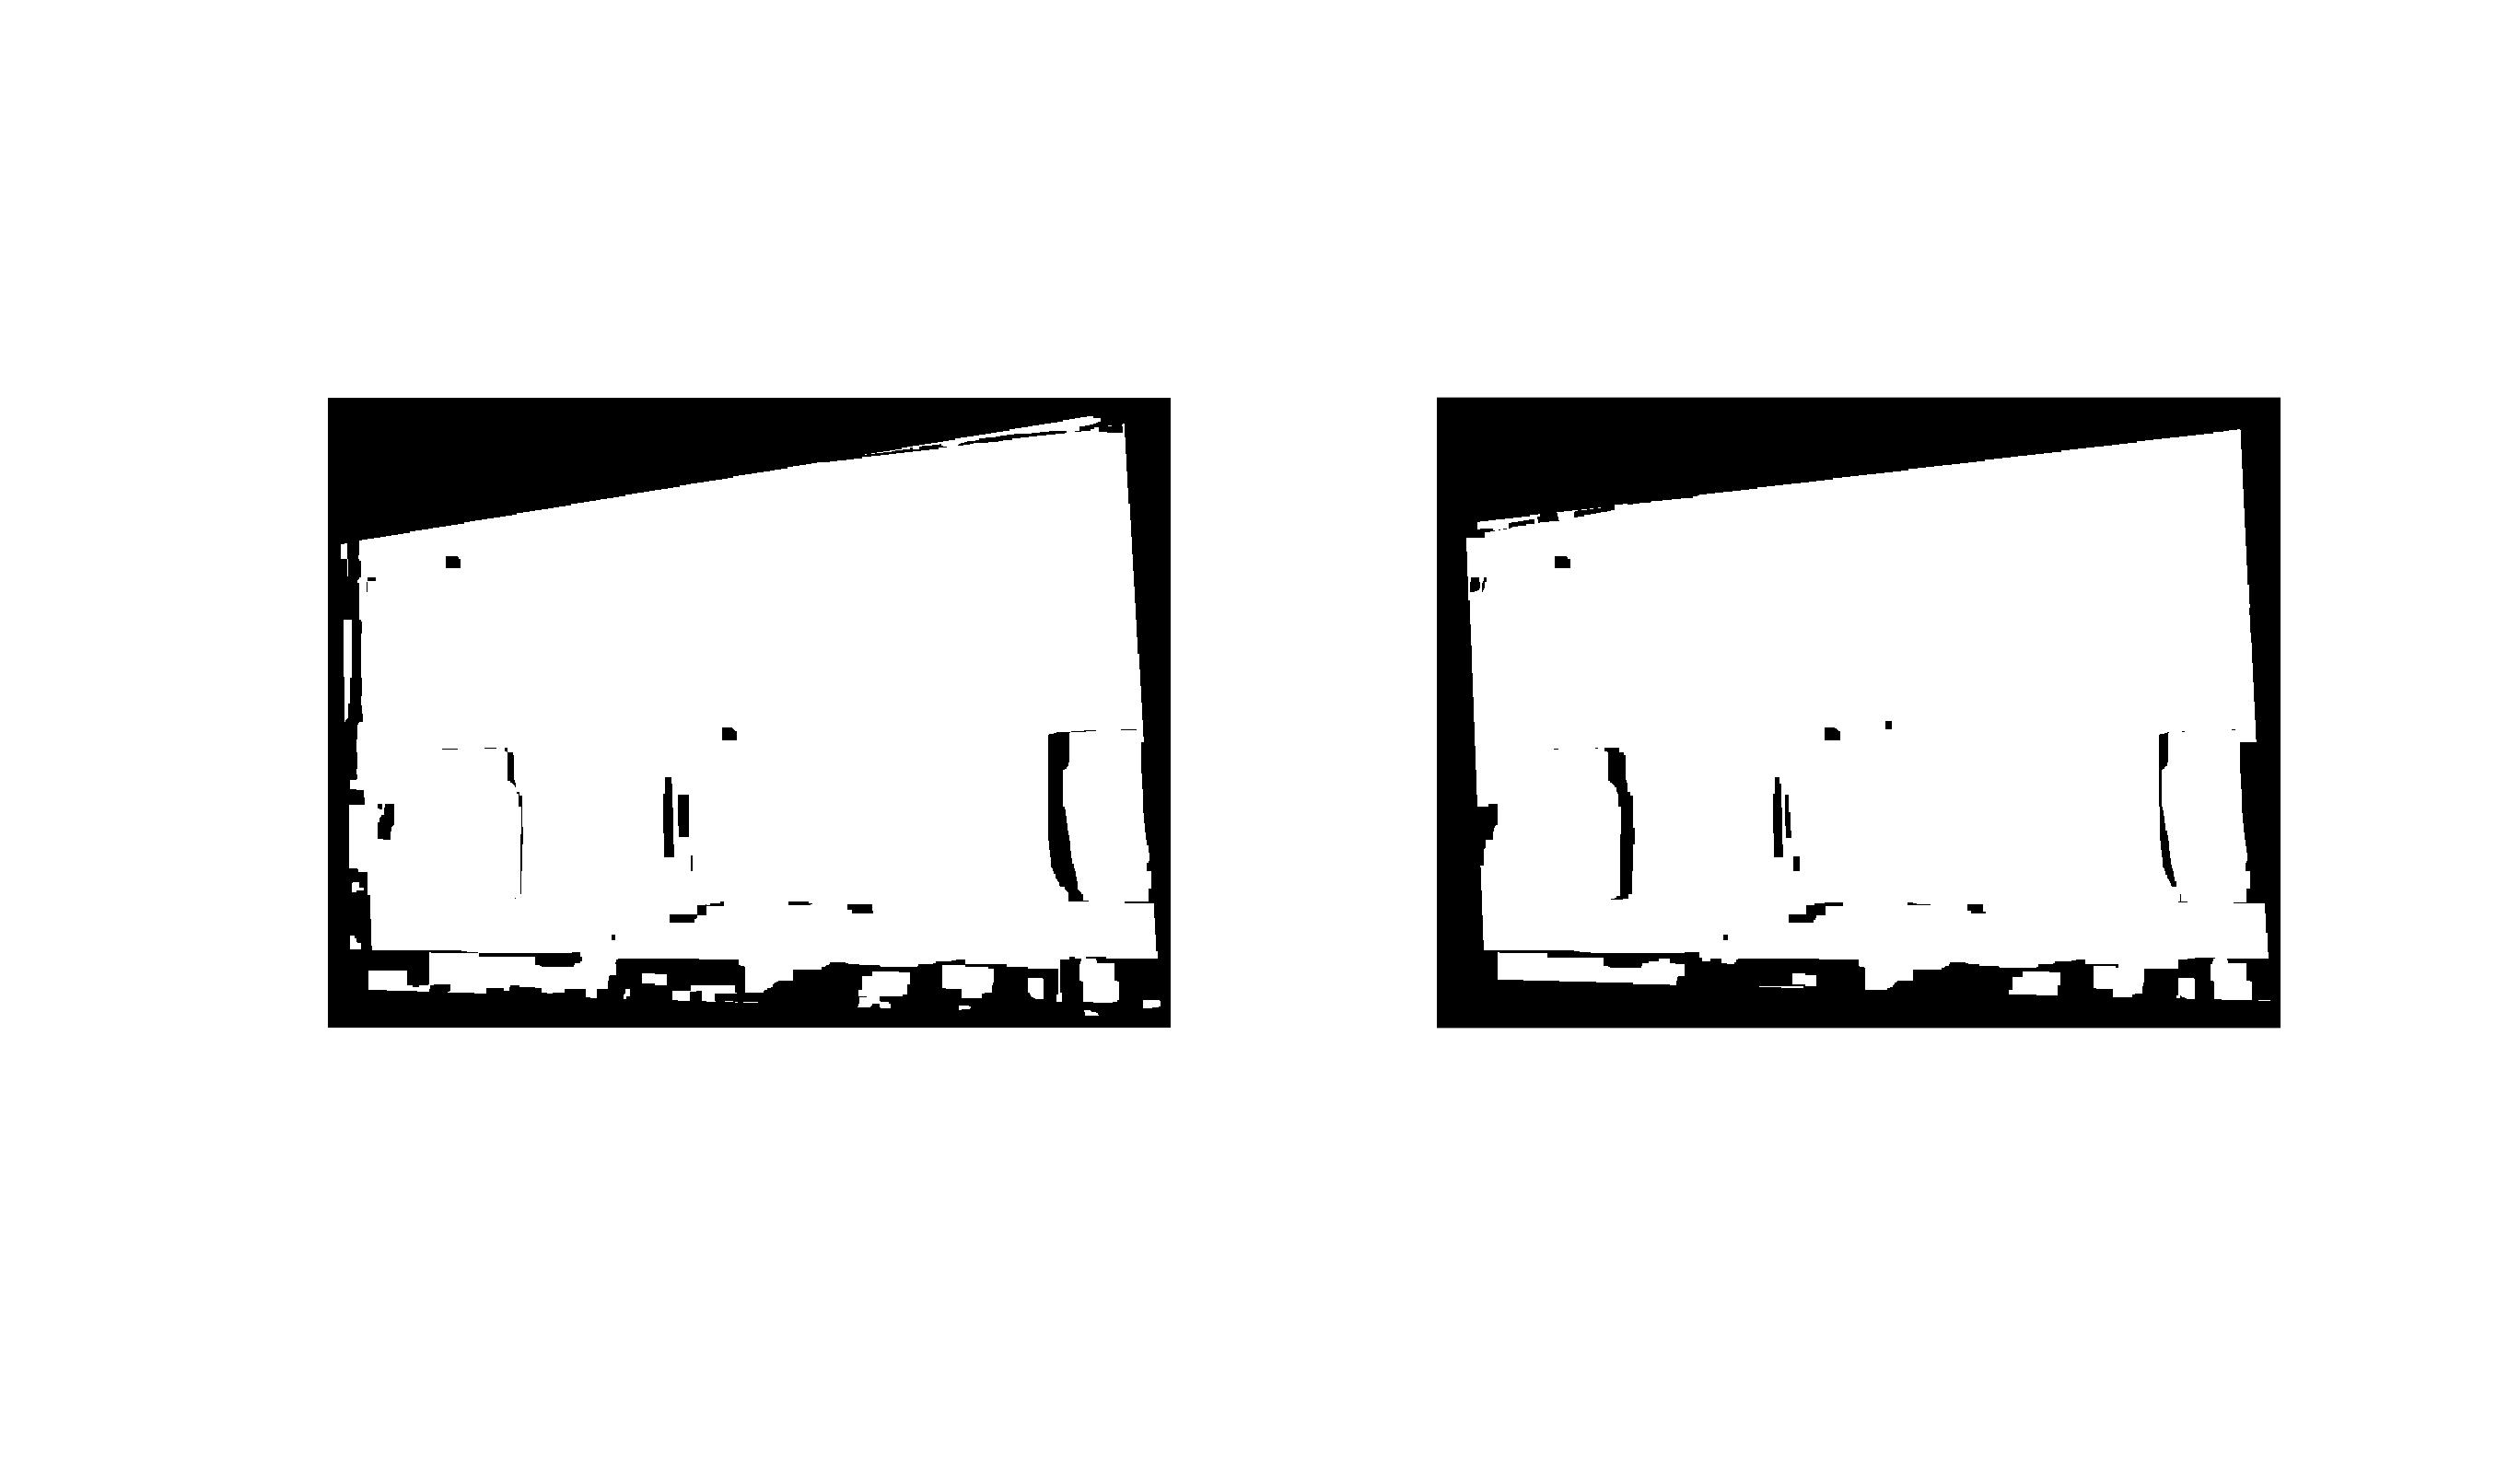
\includegraphics[width=1.1\textwidth]{gc_500_5_2.jpg}
	\caption{$DC*500$, $SC*5$}
	\label{fig1}
\end{figure}
\begin{figure}[H]
	\centering
	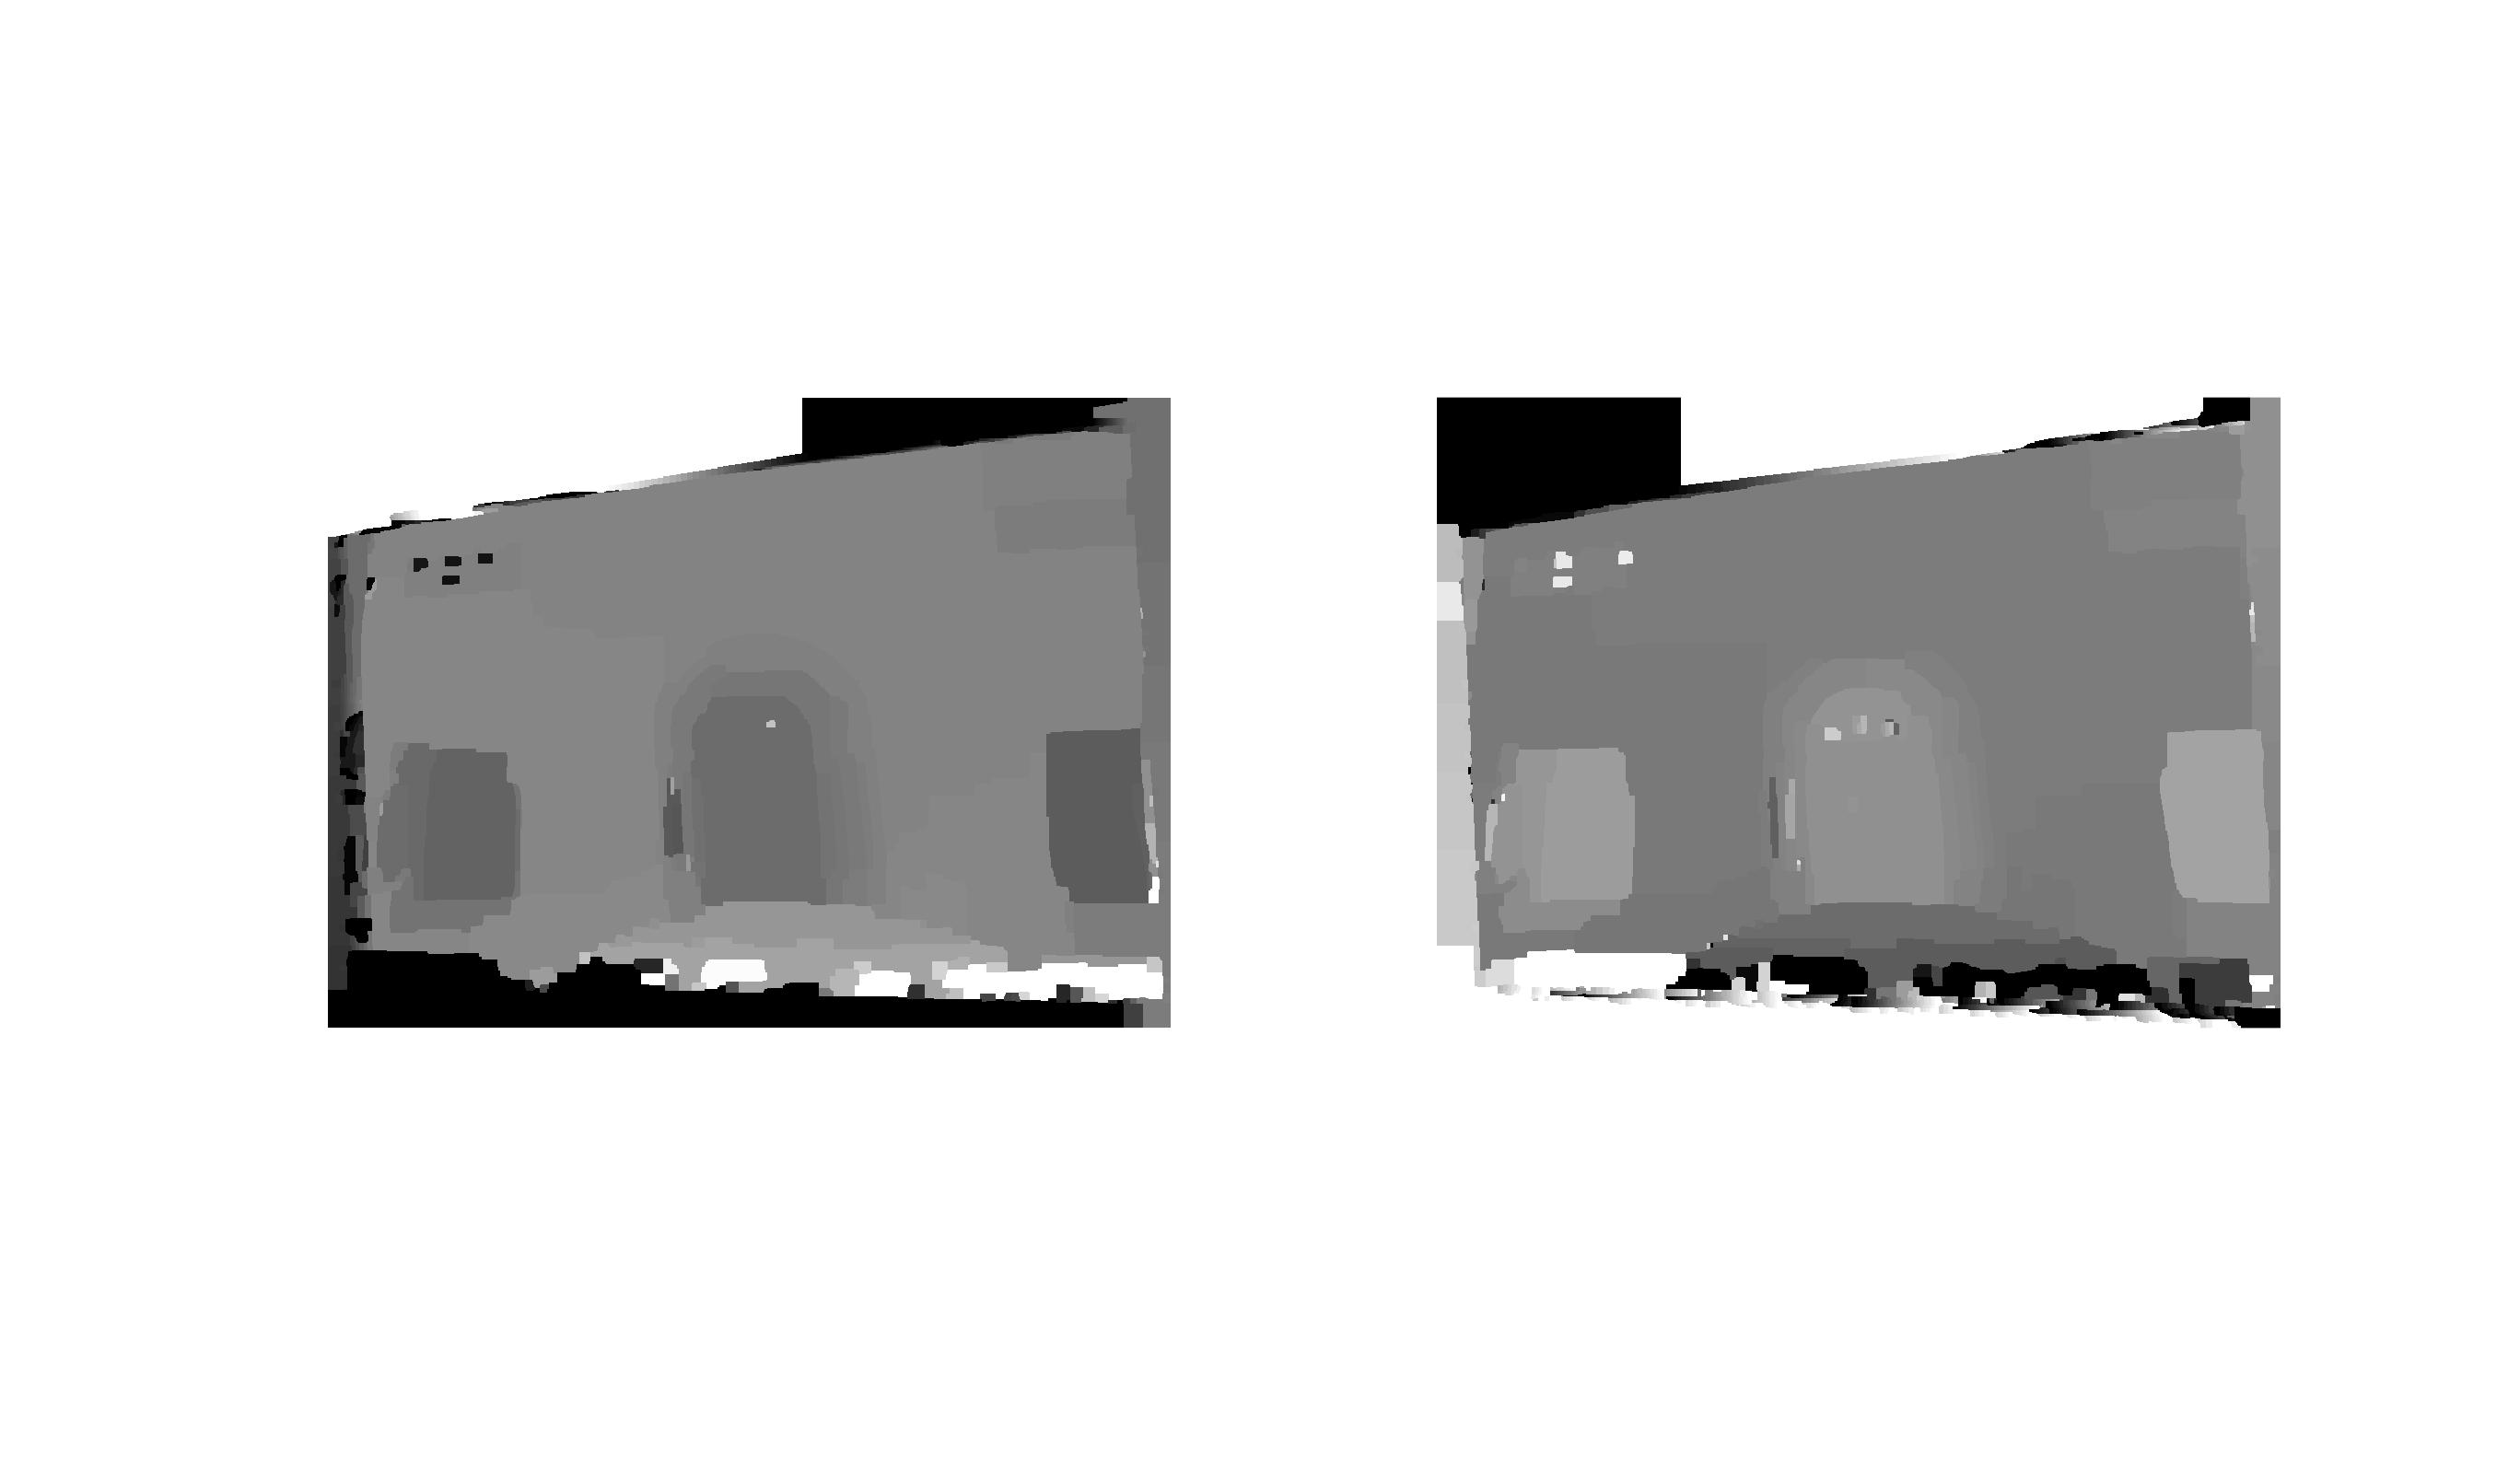
\includegraphics[width=1.1\textwidth]{gc_1000_5_1.jpg}
	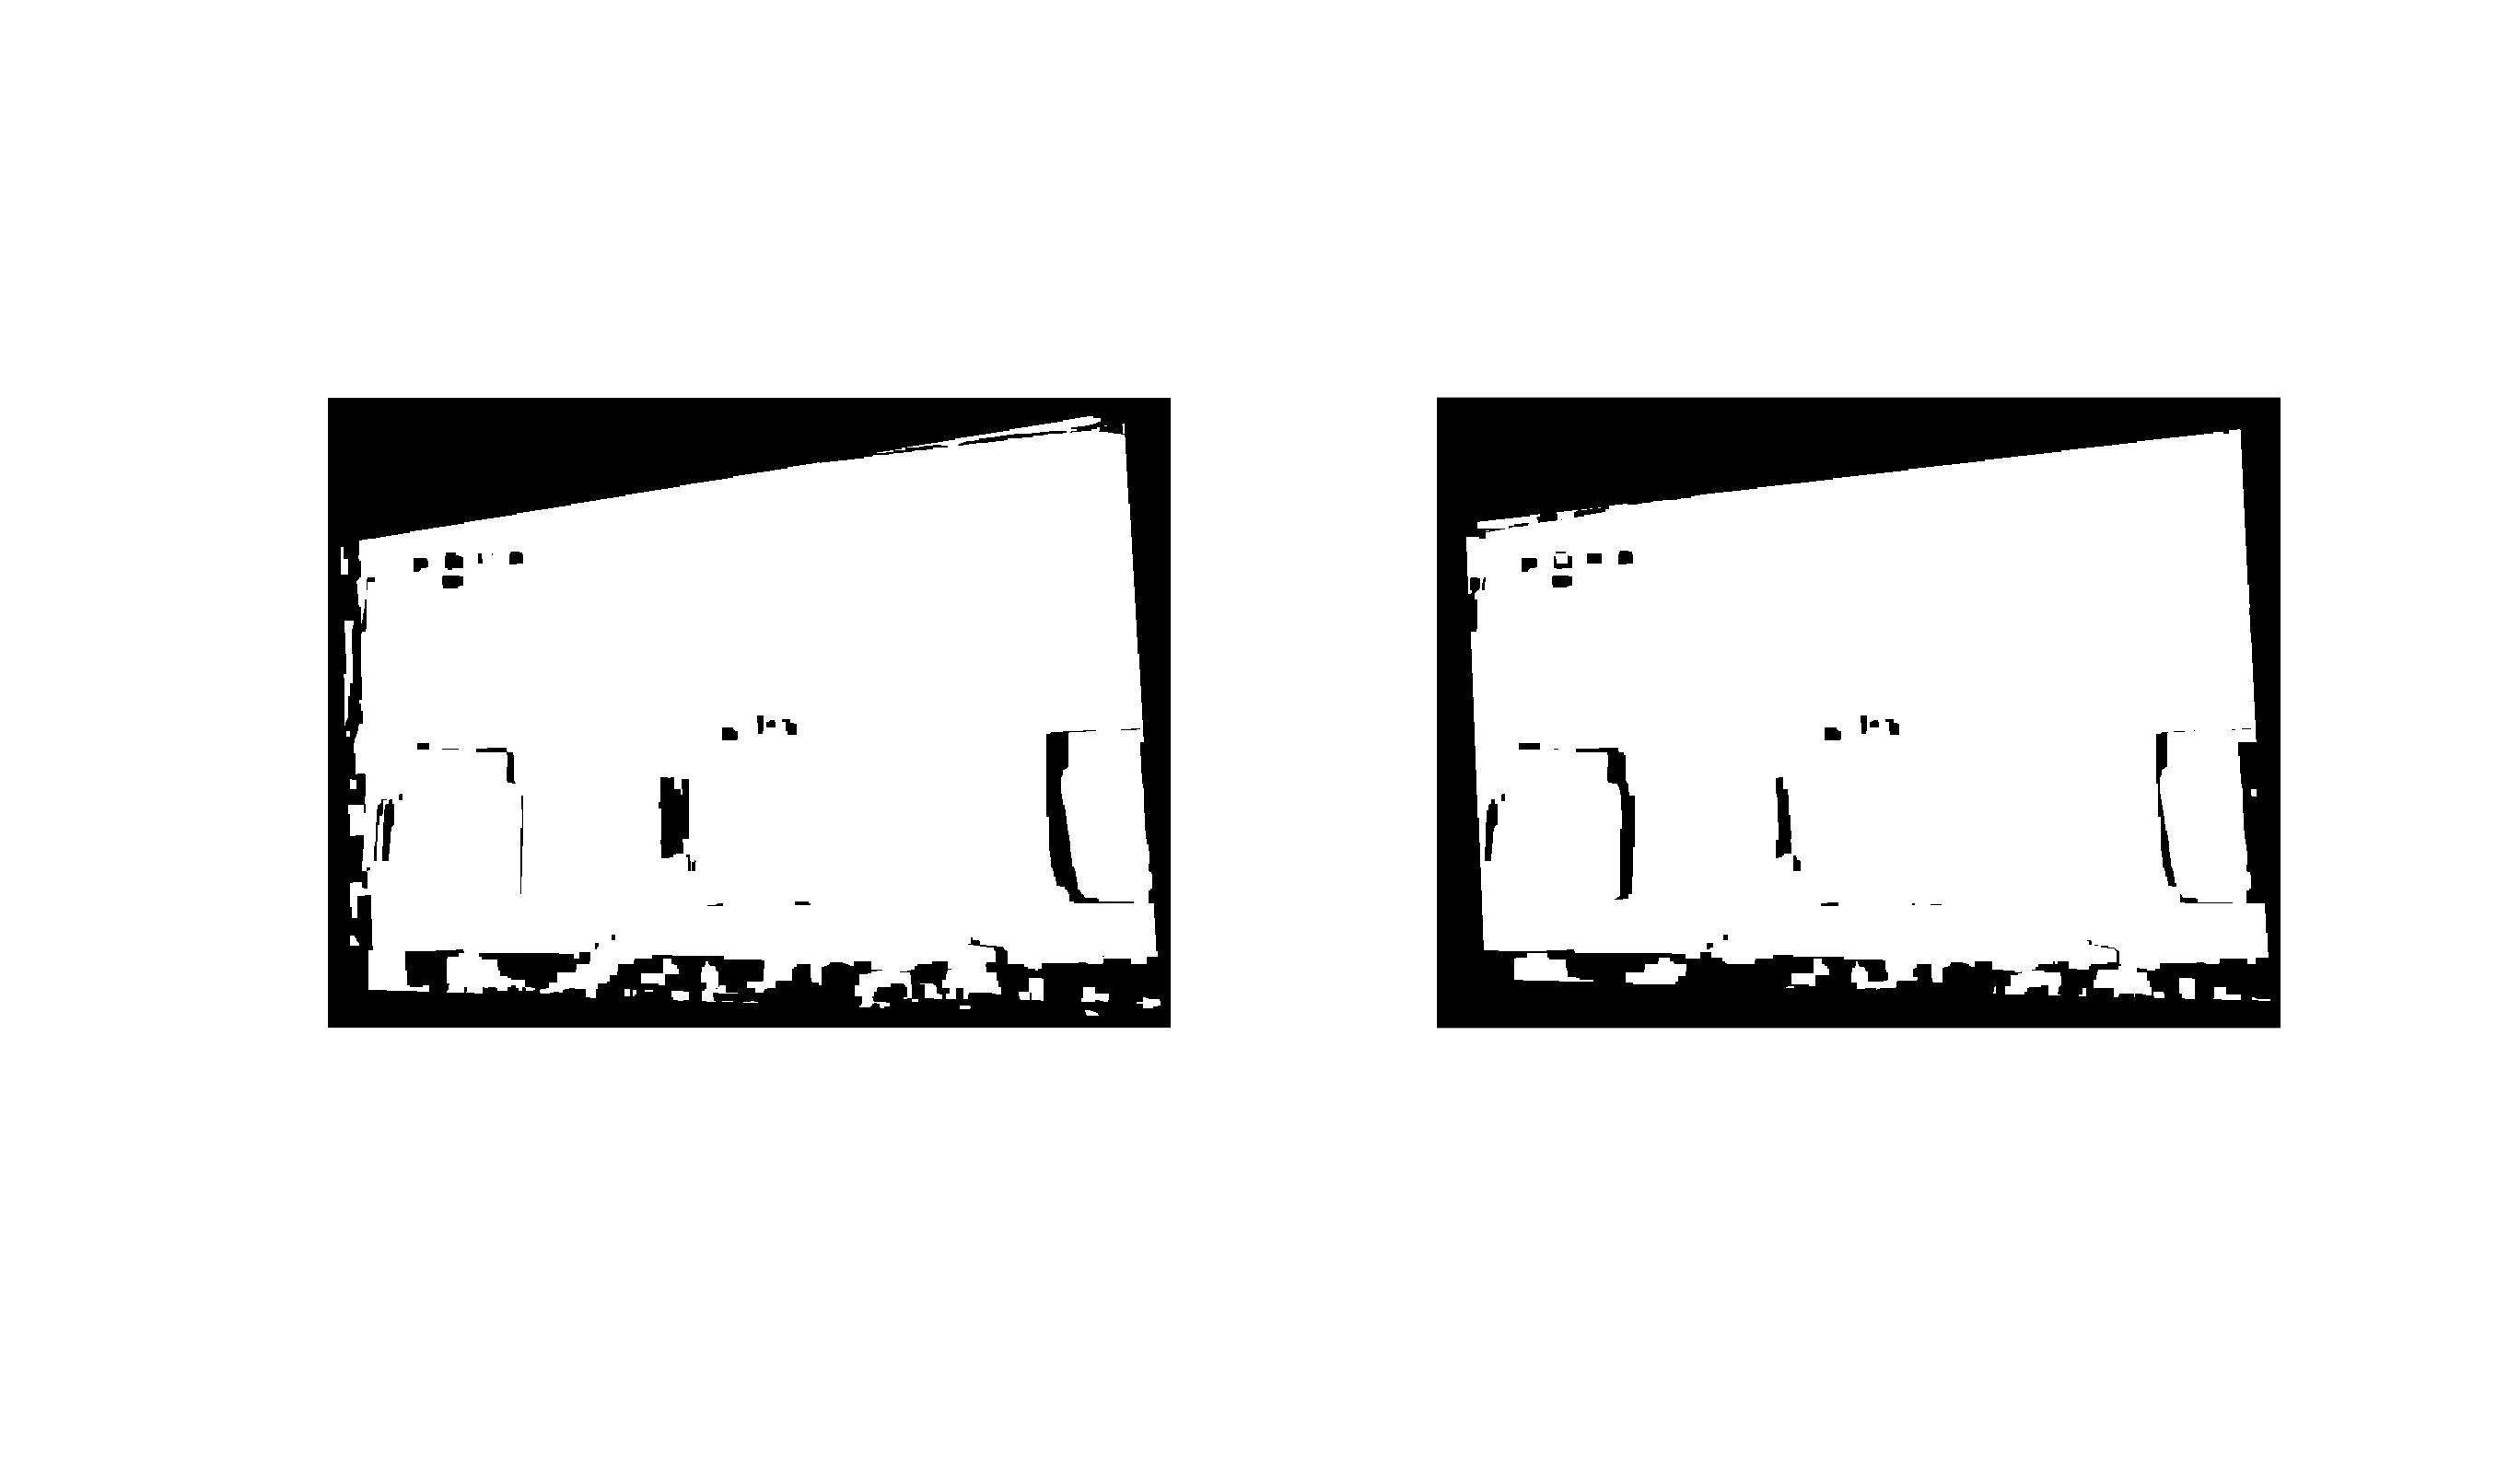
\includegraphics[width=1.1\textwidth]{gc_1000_5_2.jpg}
	\caption{$DC*1000$, $SC*5$}
	\label{fig1}
\end{figure}
\begin{figure}[H]
	\centering
	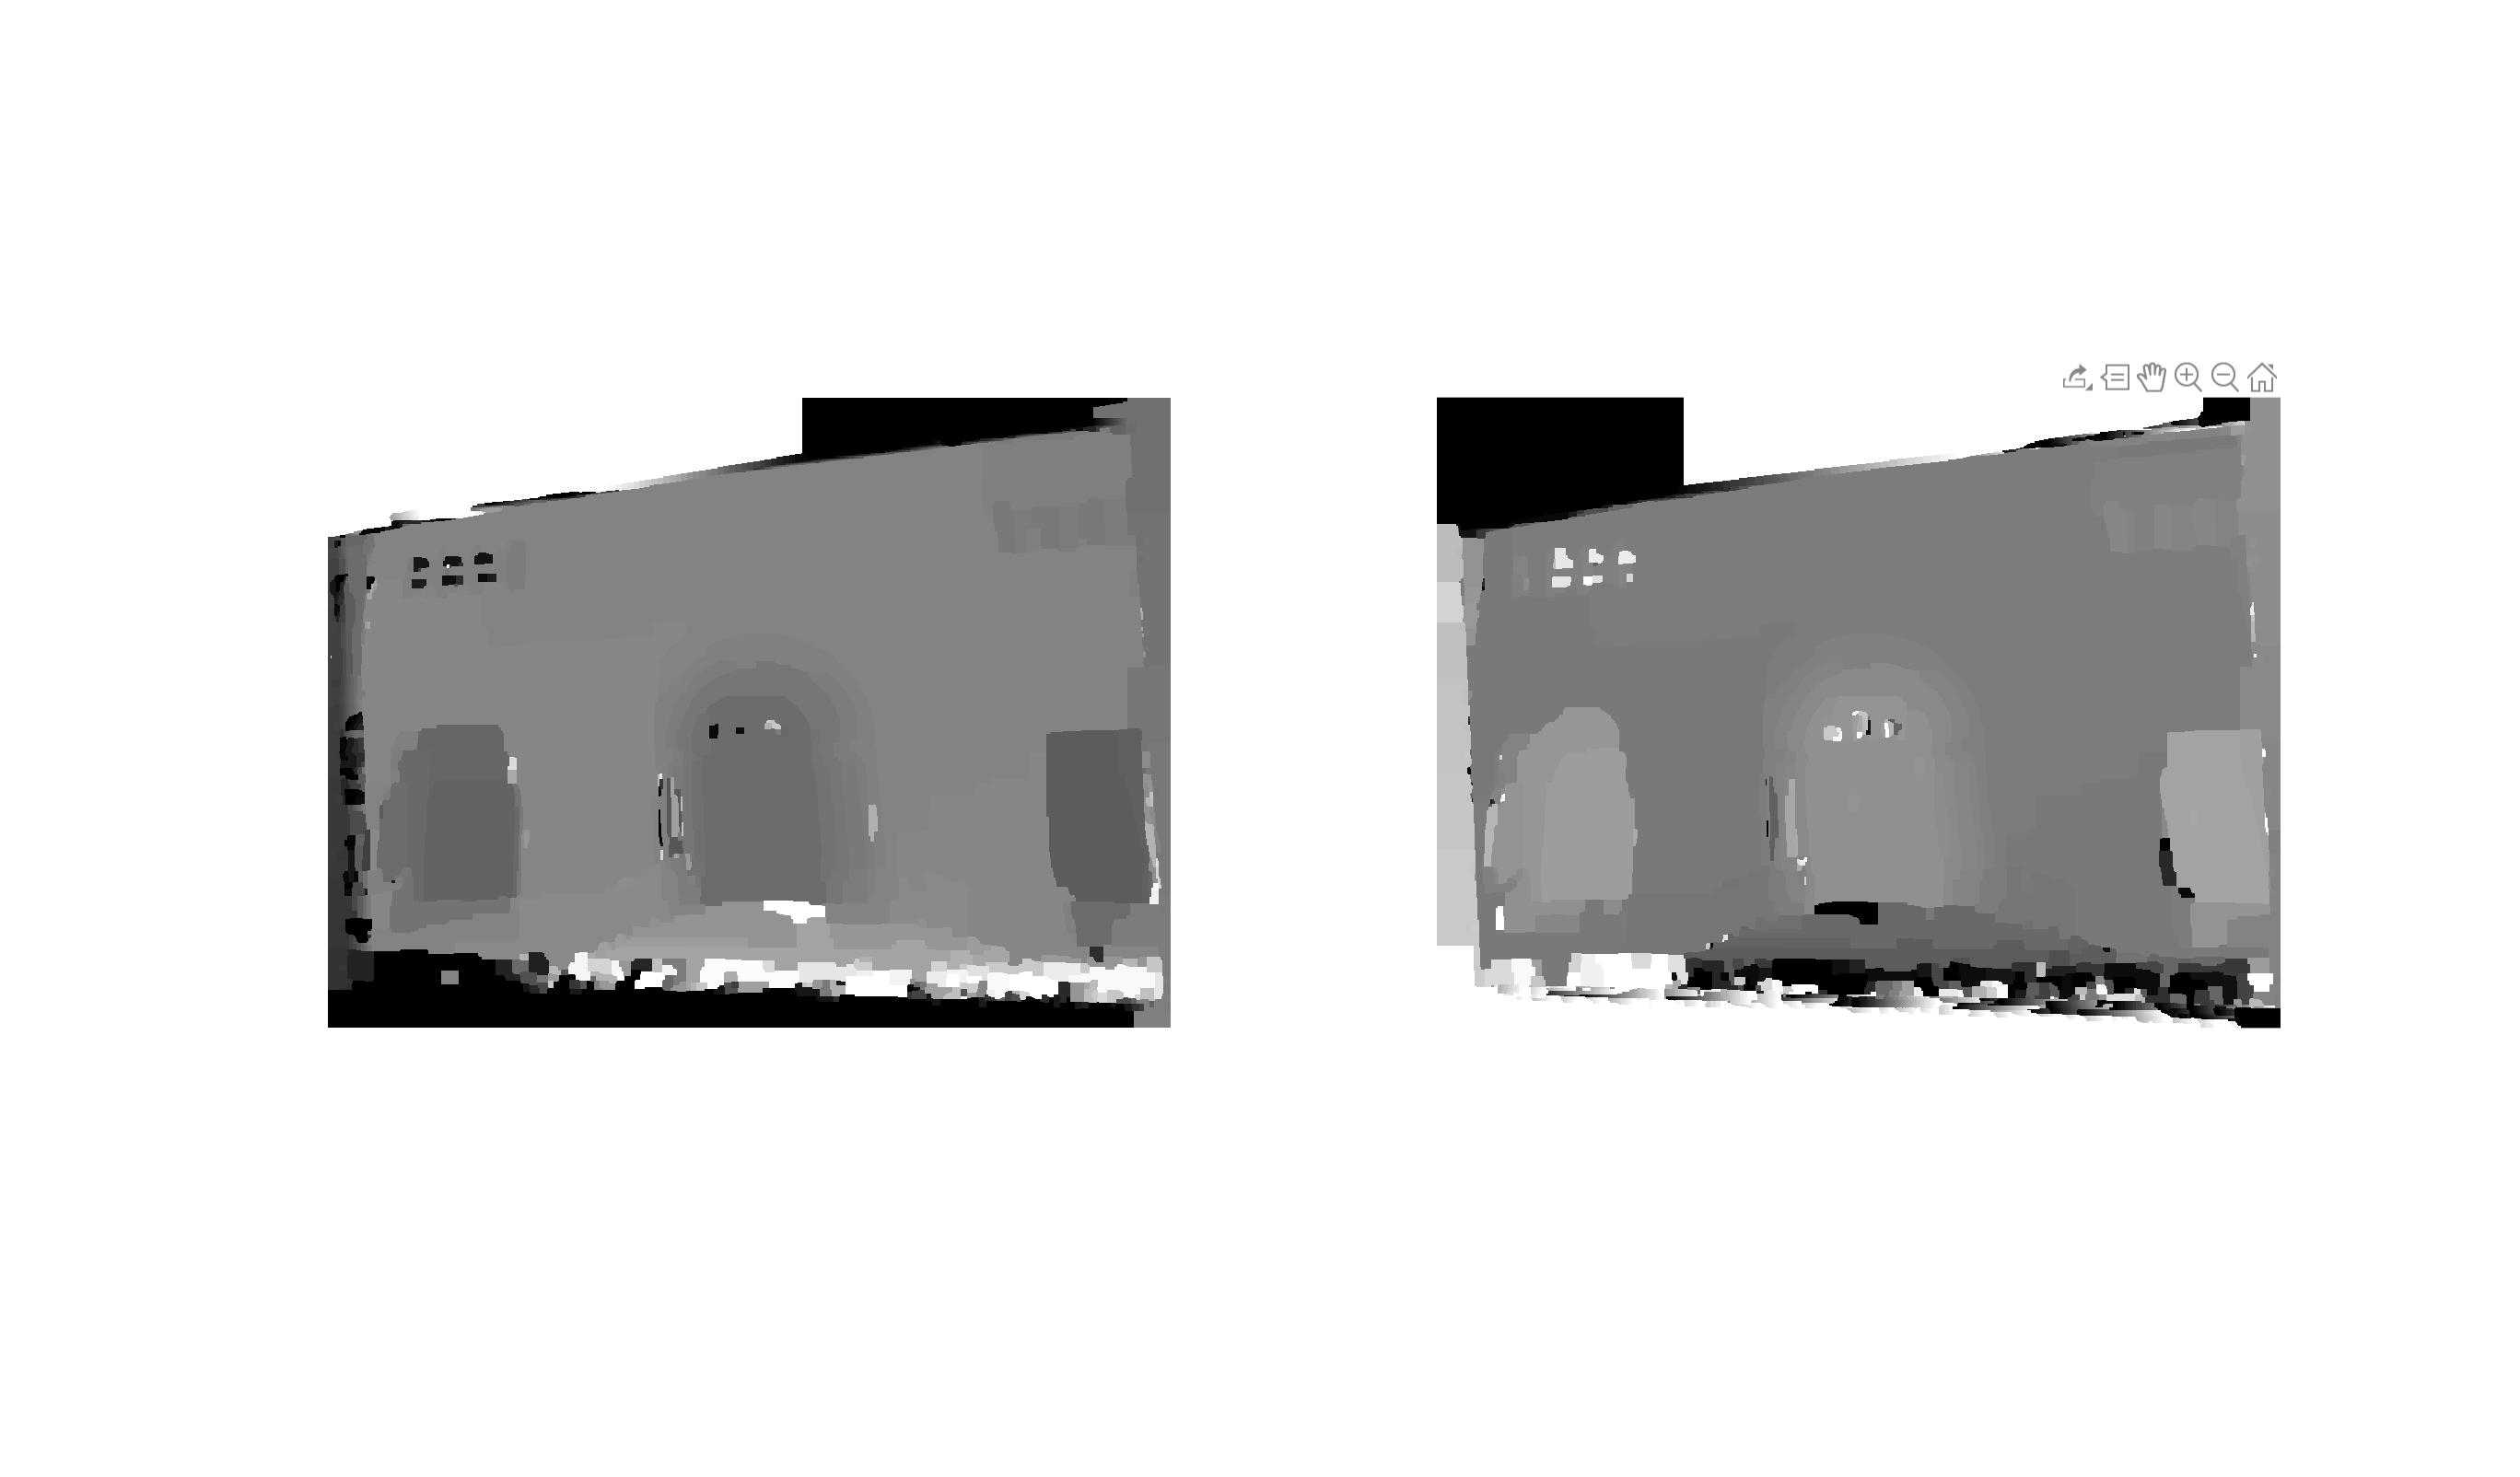
\includegraphics[width=1.1\textwidth]{gc_2000_5_1.jpg}
	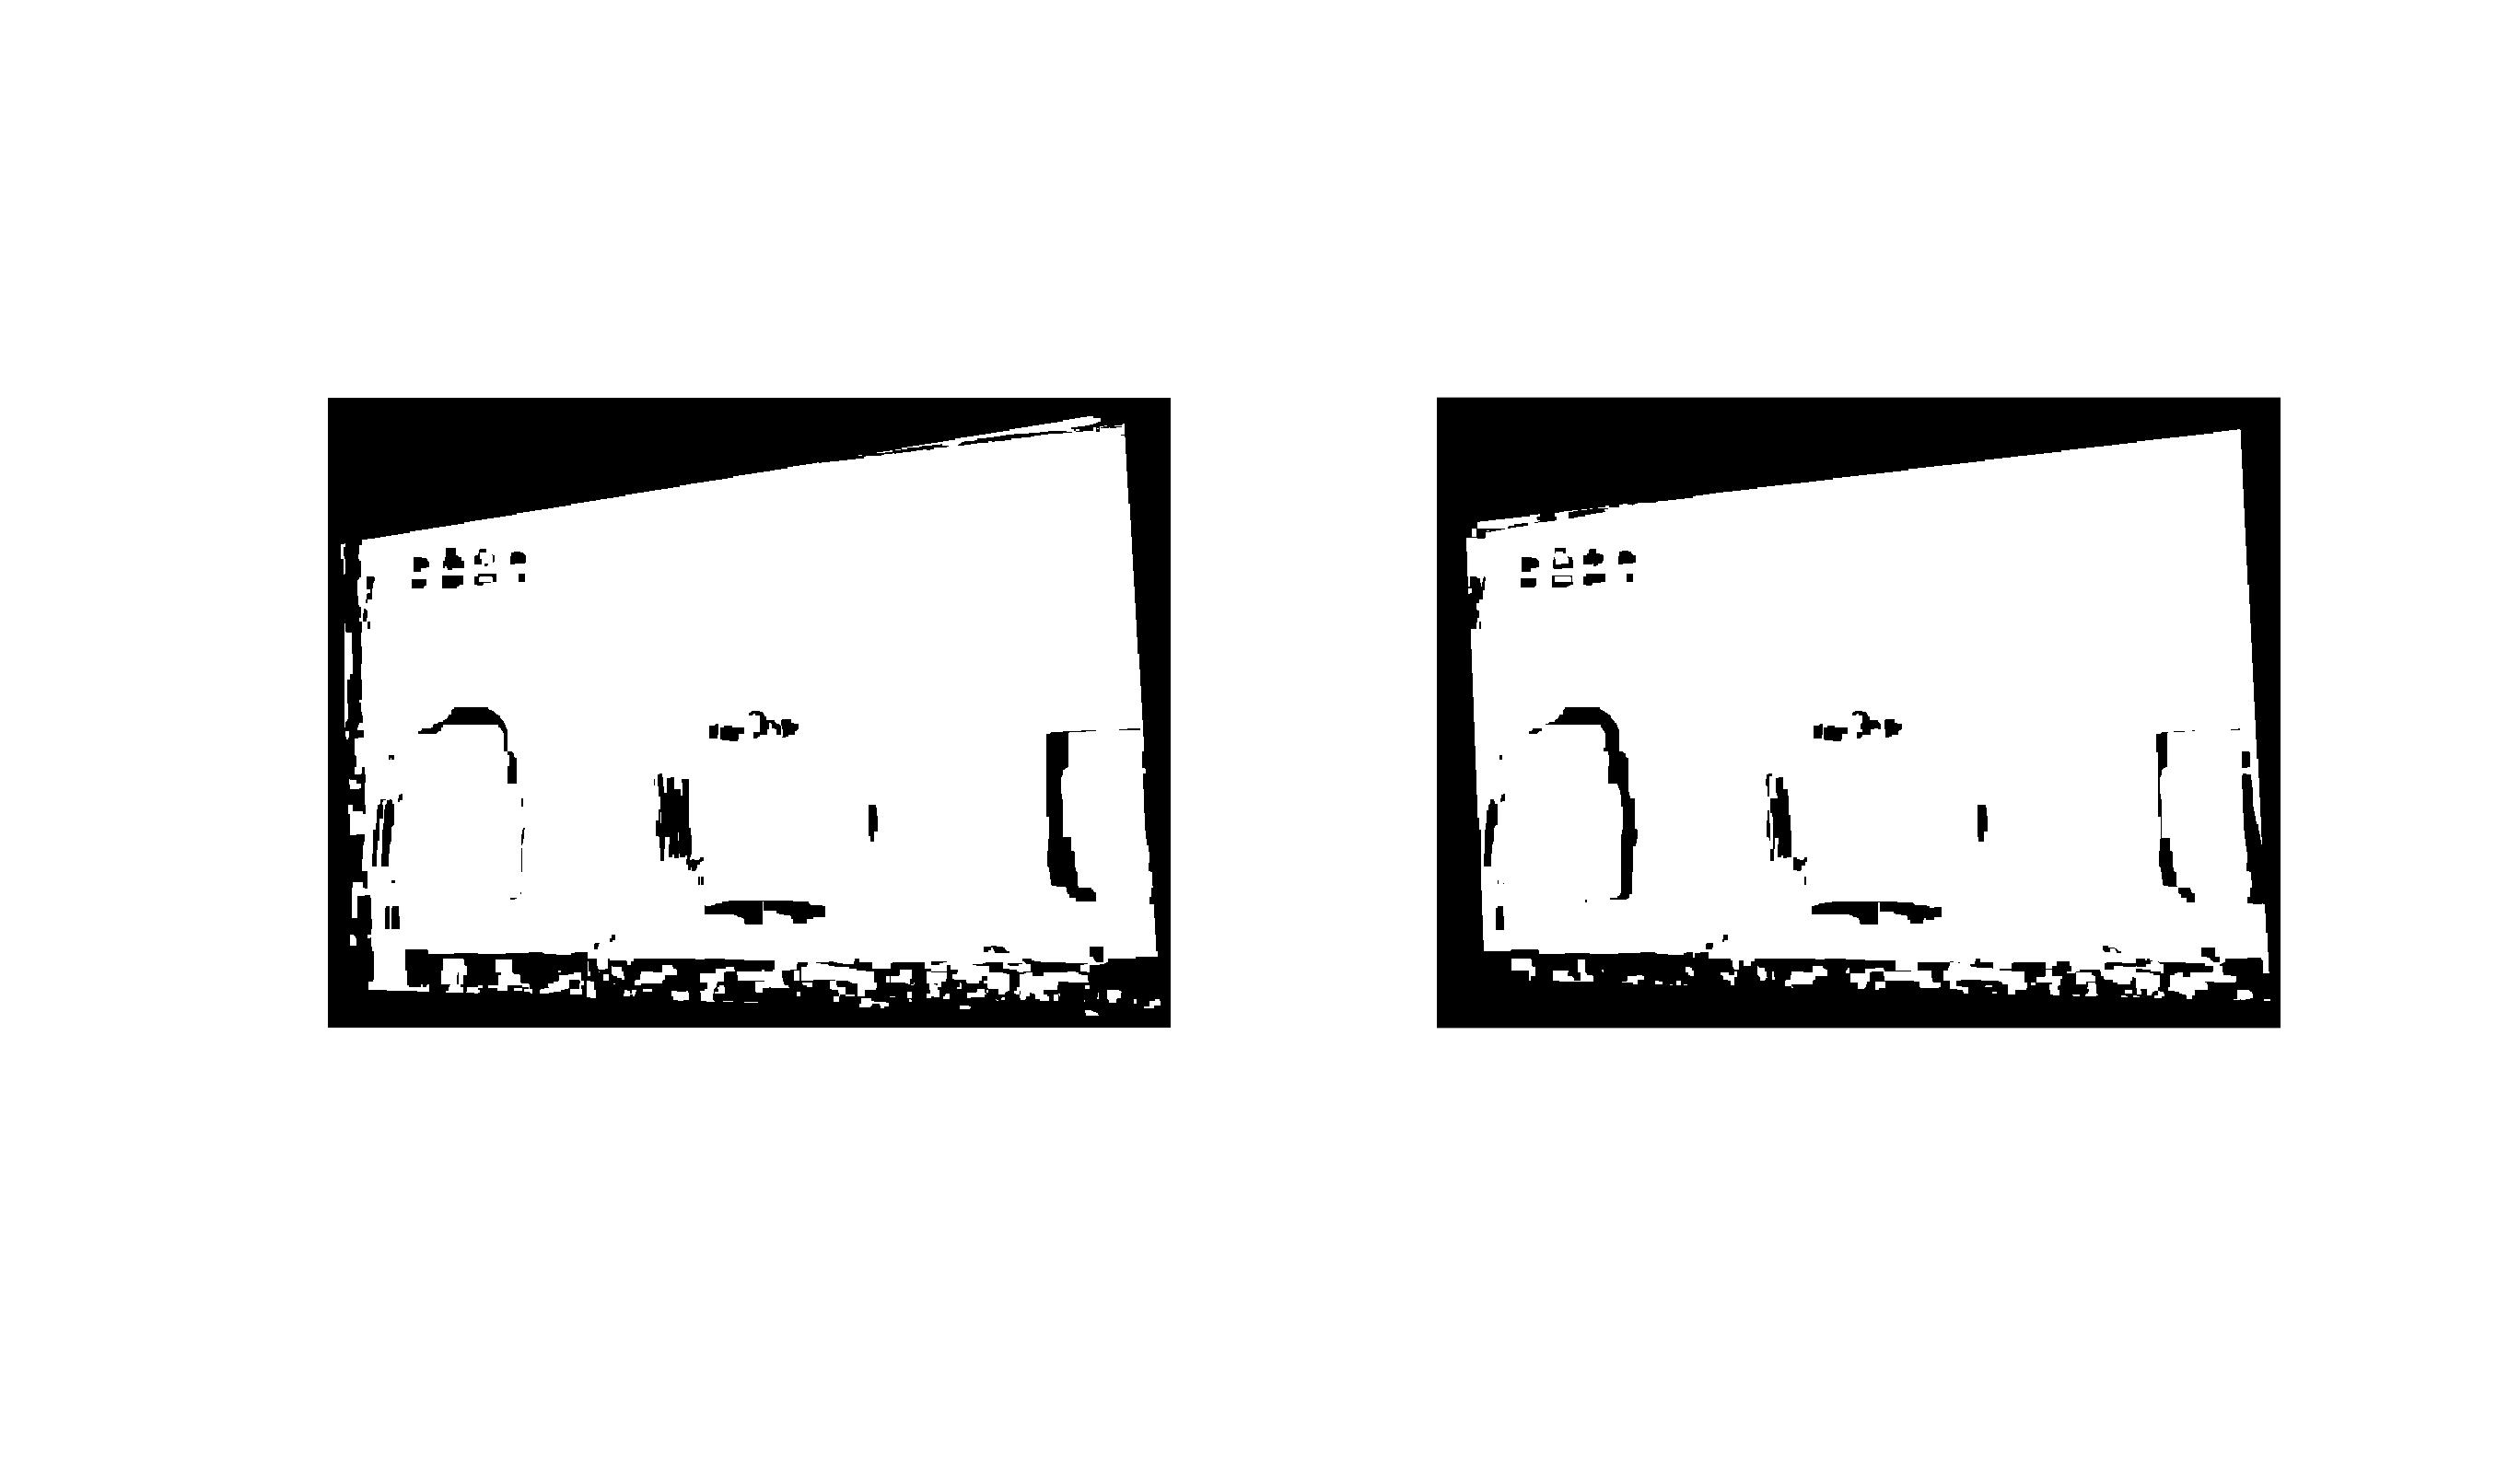
\includegraphics[width=1.1\textwidth]{gc_2000_5_2.jpg}
	\caption{$DC*2000$, $SC*5$}
	\label{fig1}
\end{figure}
\vspace{5mm}

As can be seen in the images above a $DC_factor$ of 500 performed best for producing a continuous image. No definitive conclusion about the accuracy can be made without the measurements of the building.
\vspace{5mm}
\newline
Here are a few of the tried results with variation of SC: 
\vspace{5mm}
\begin{figure}[H]
	\centering
	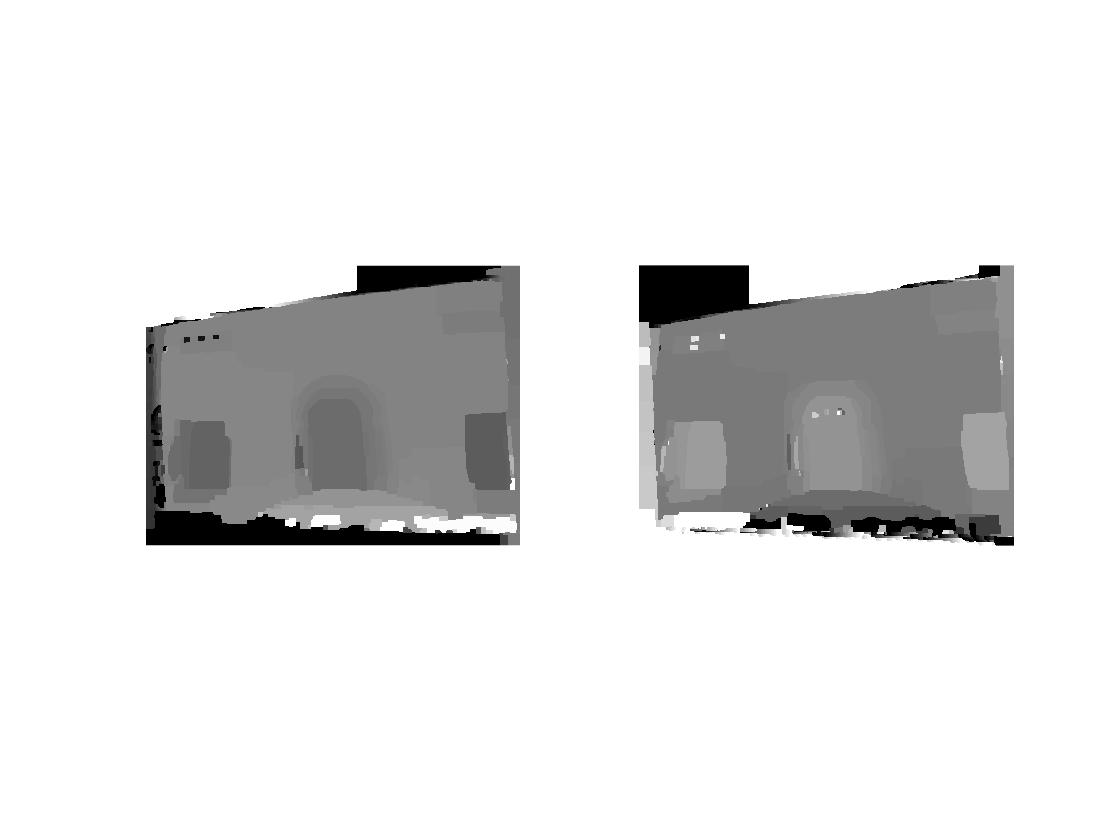
\includegraphics[width=1.1\textwidth]{gc_500_3_1.jpg}
	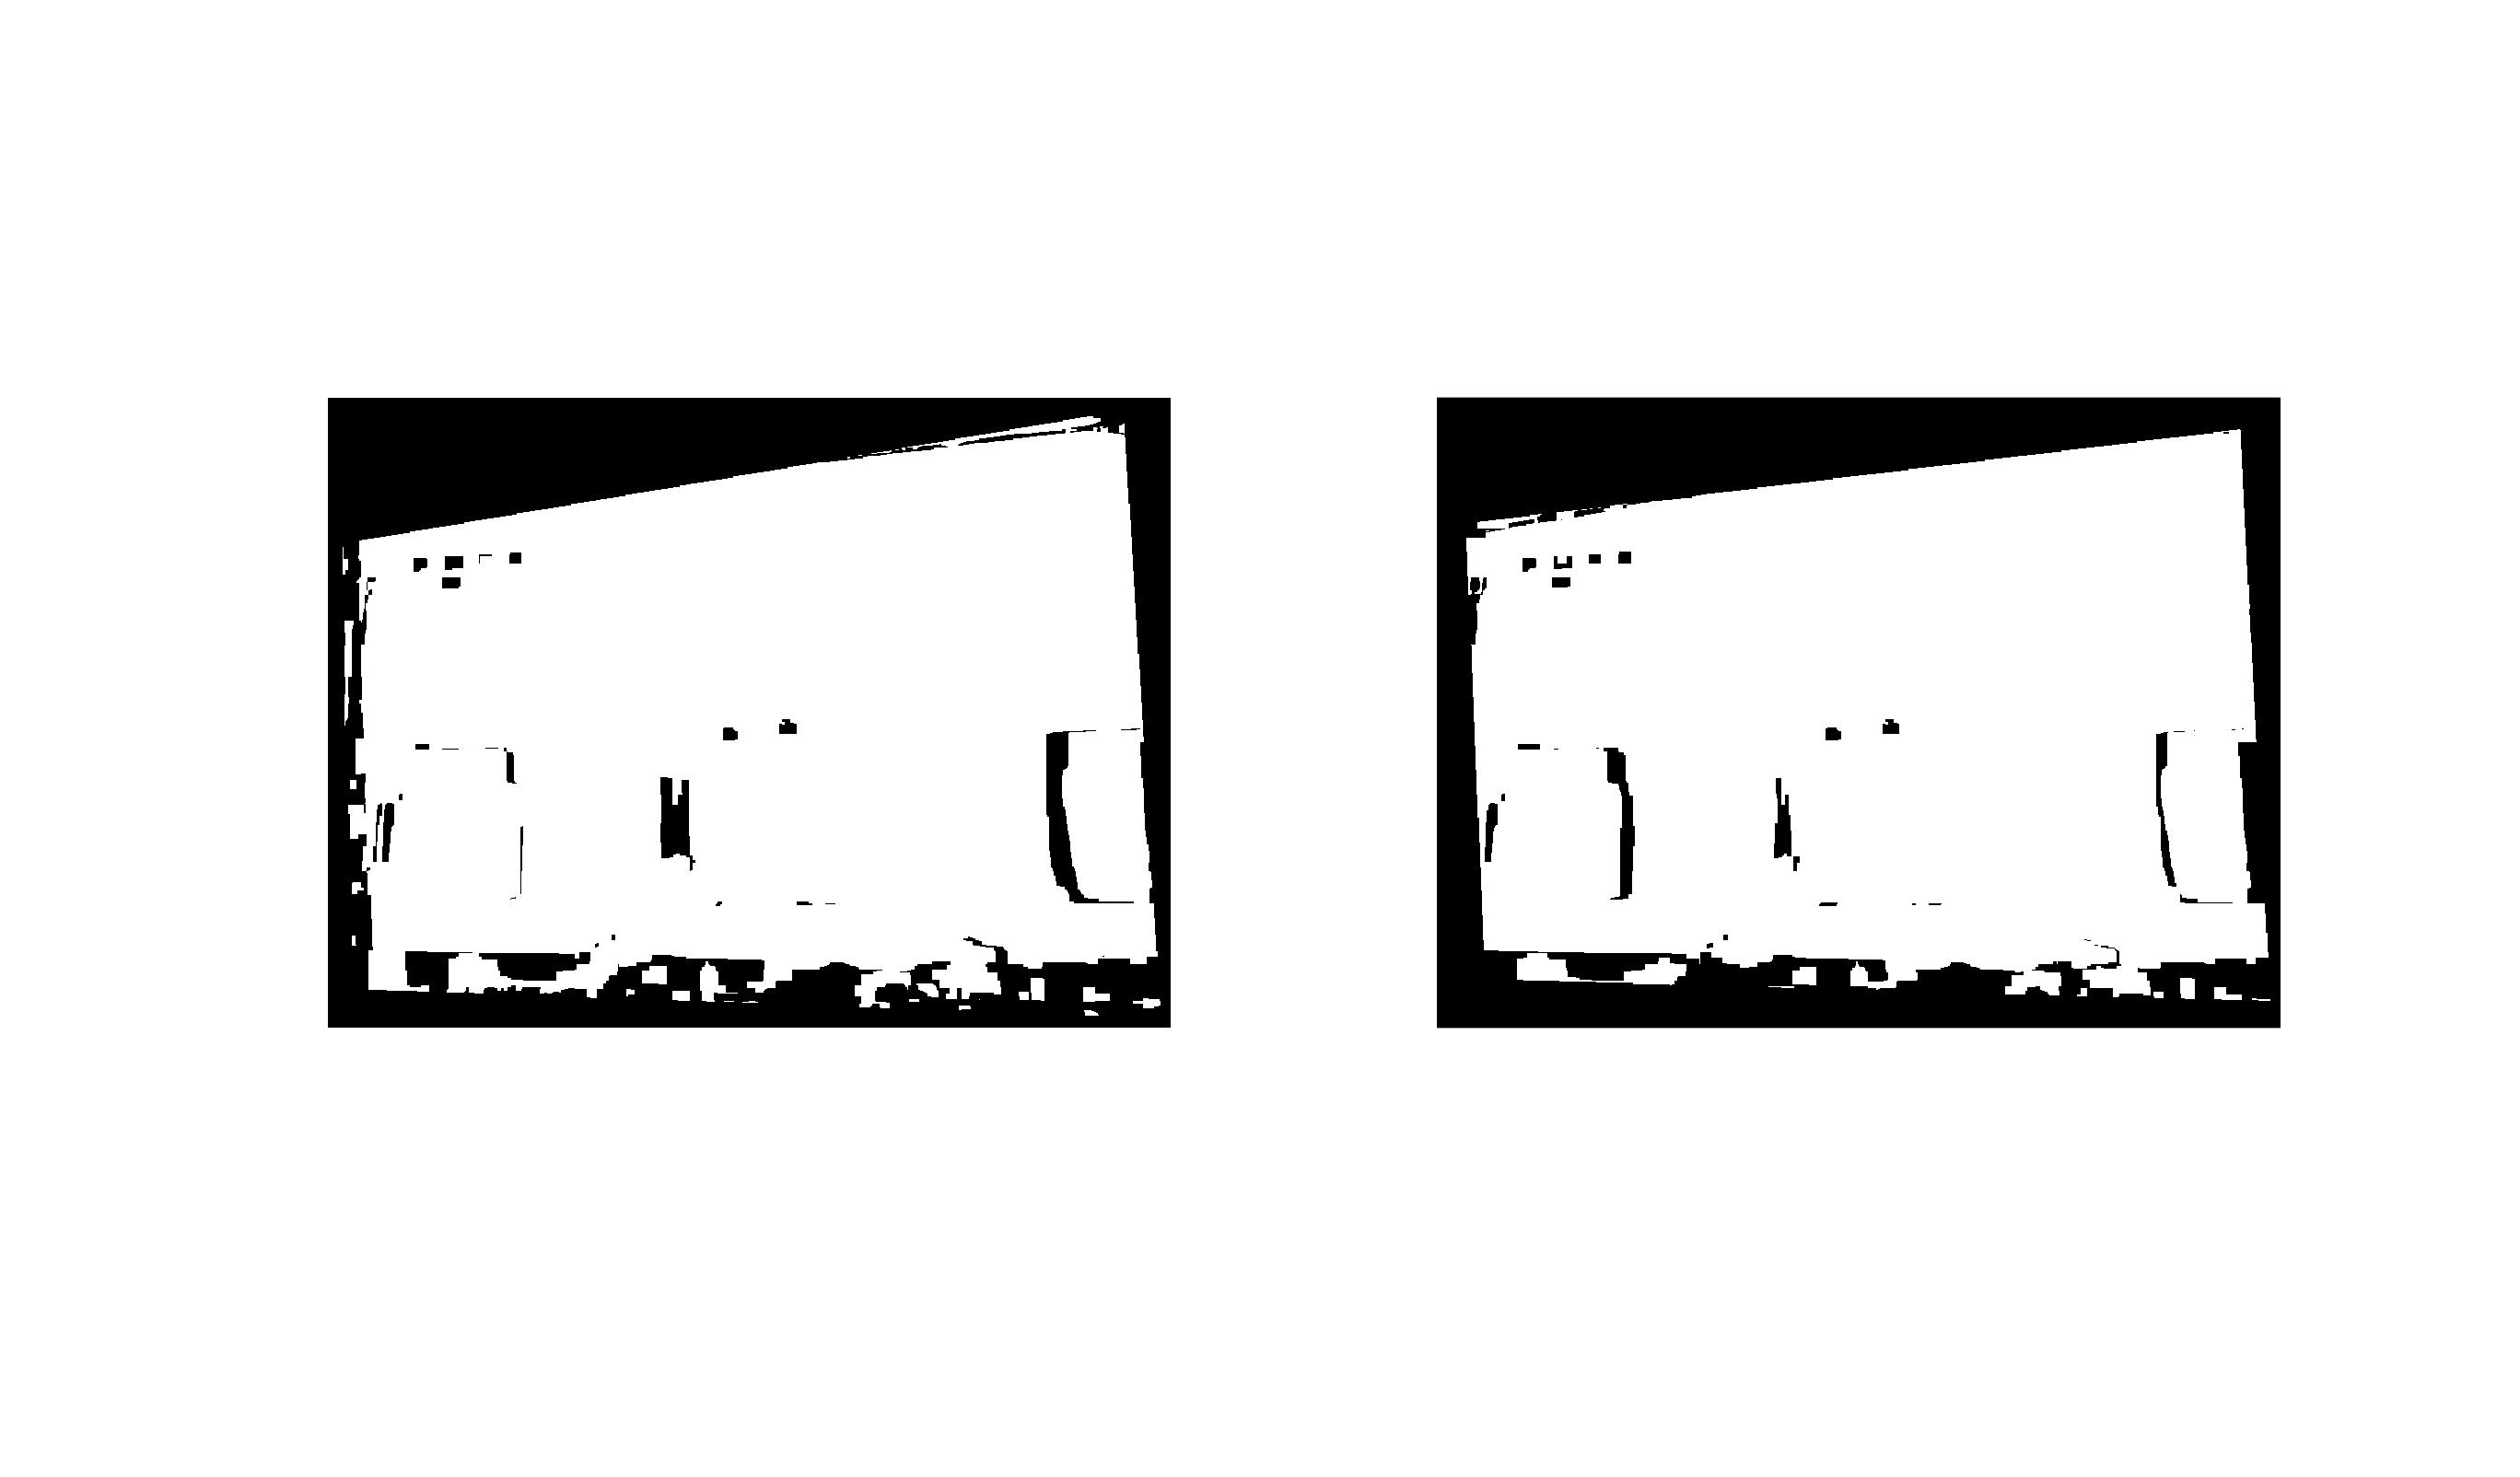
\includegraphics[width=1.1\textwidth]{gc_500_3_2.jpg}
	\caption{$DC*500$, $SC*3$}
	\label{fig1}
\end{figure}
\vspace{5mm}
\begin{figure}[H]
	\centering
	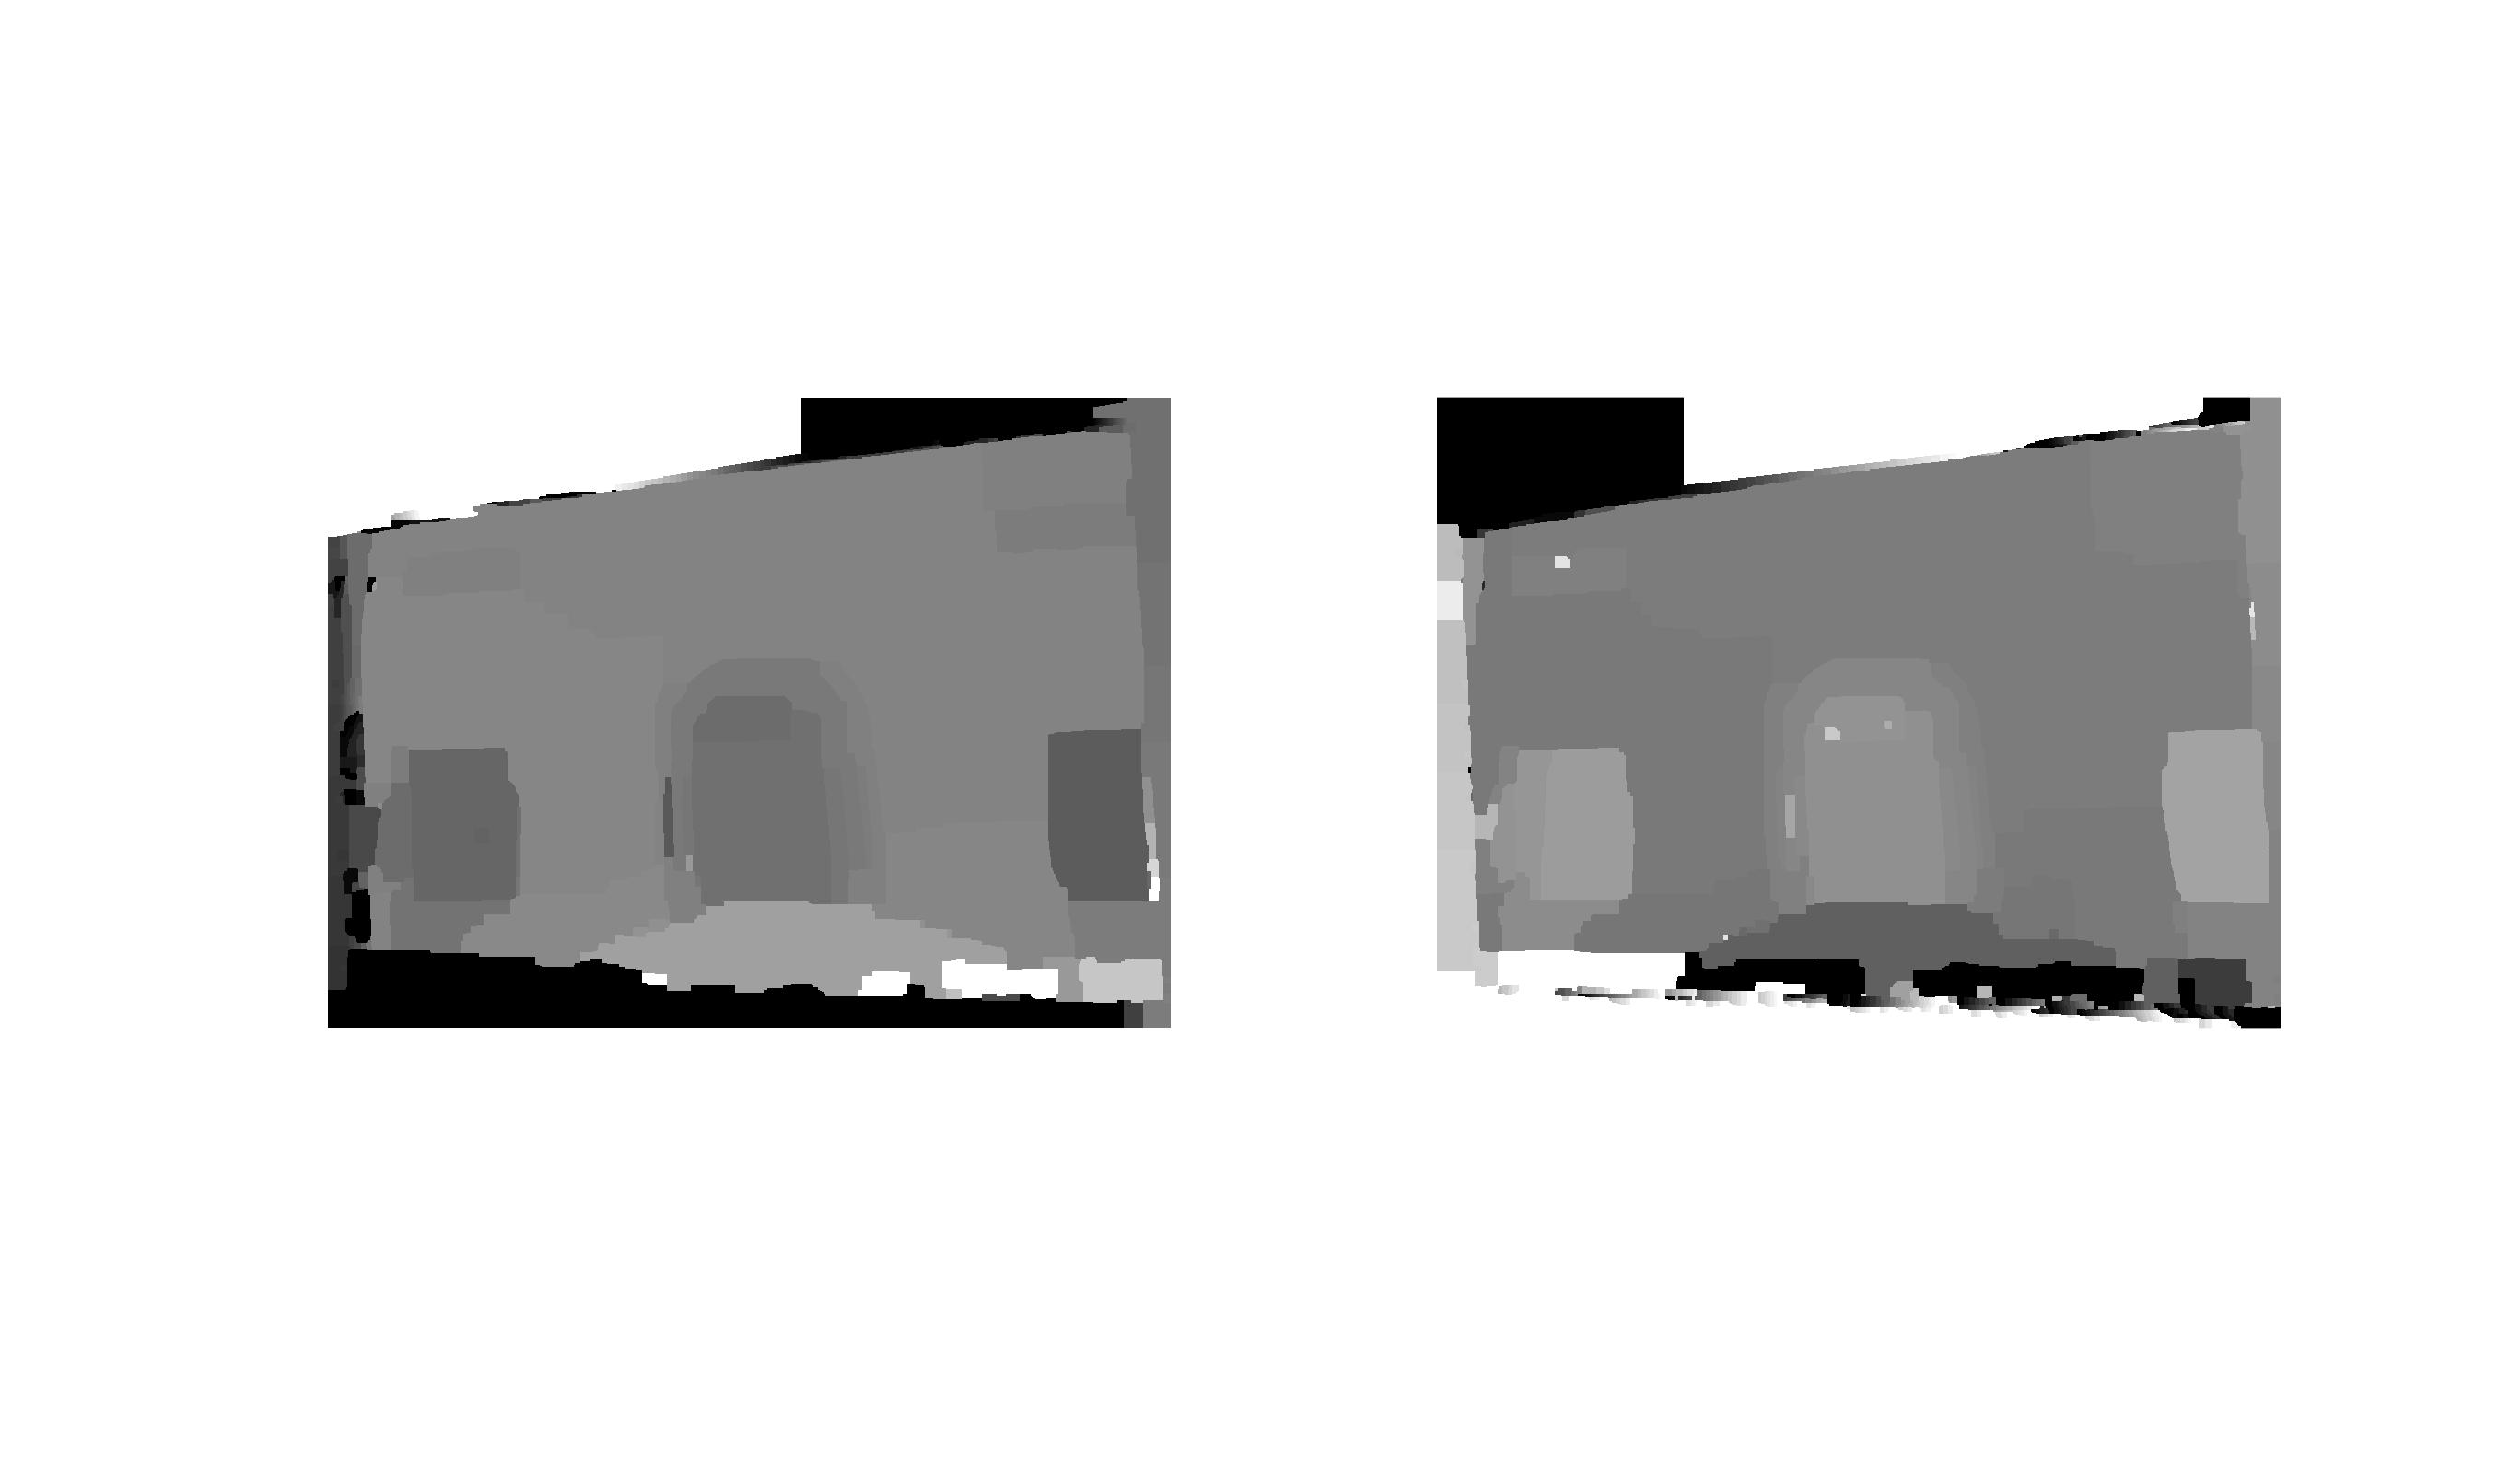
\includegraphics[width=1.1\textwidth]{gc_500_5_1.jpg}
	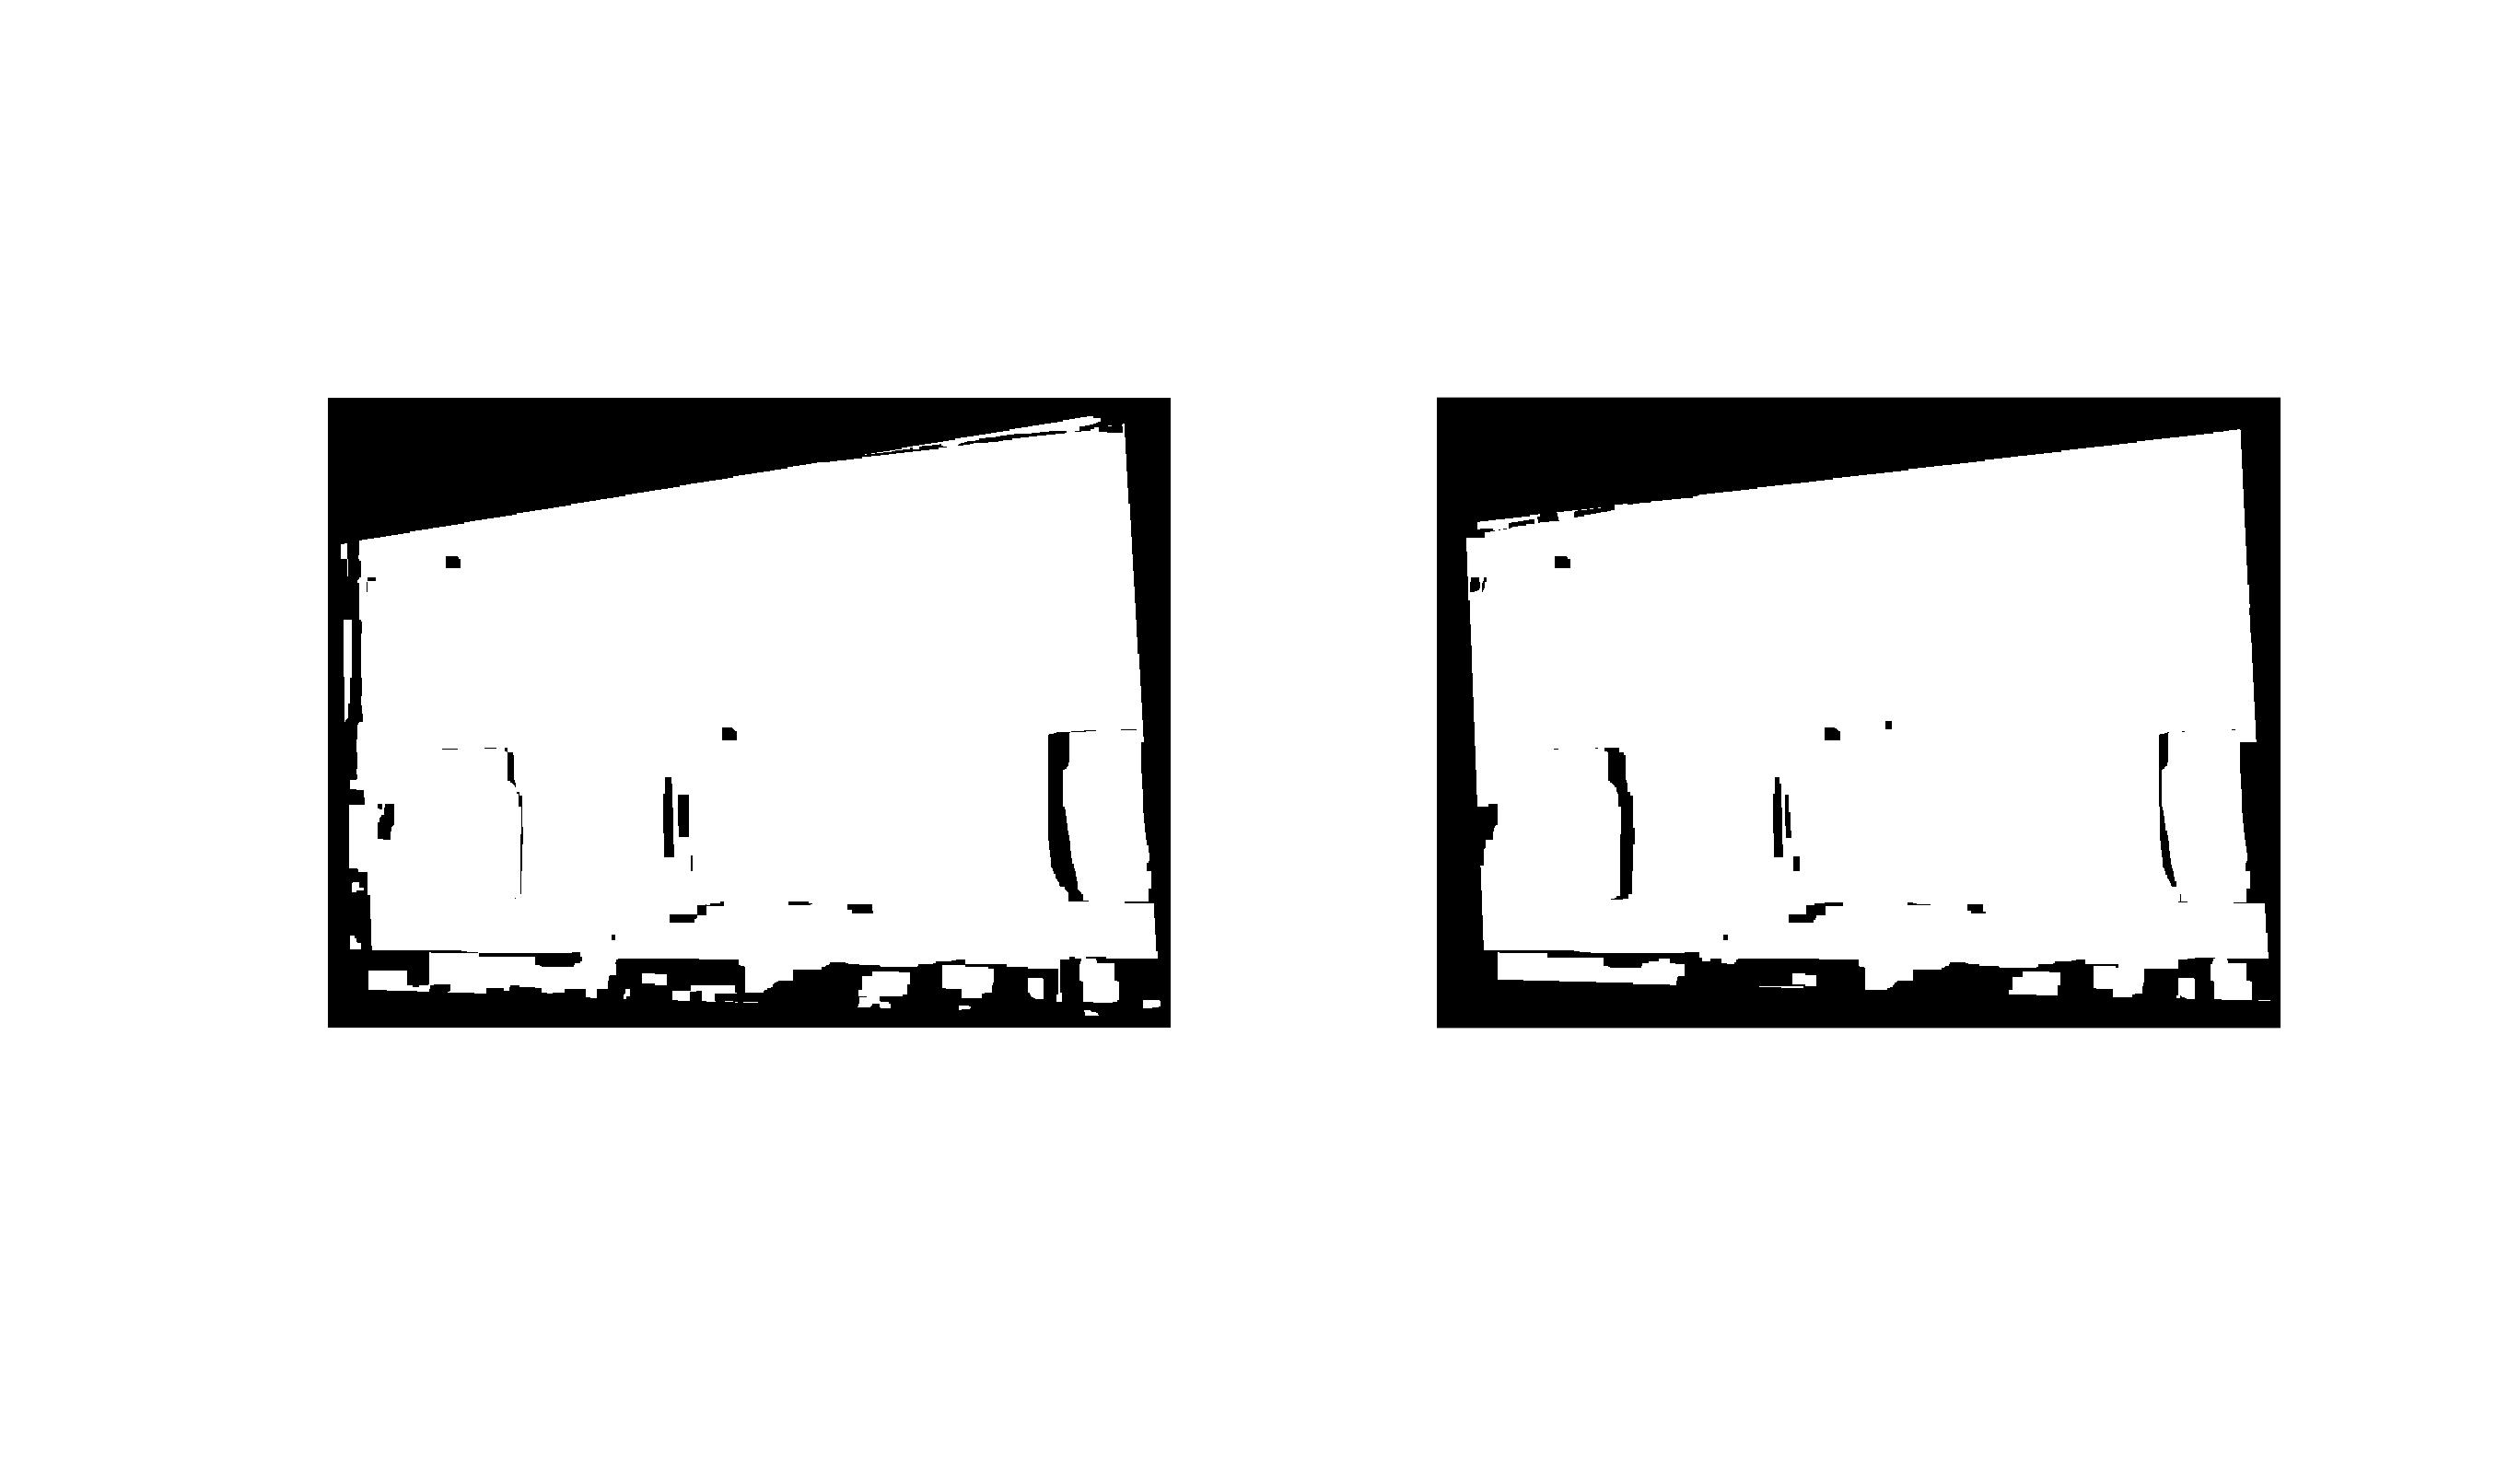
\includegraphics[width=1.1\textwidth]{gc_500_5_2.jpg}
	\caption{$DC*500$, $SC*5$}
	\label{fig1}
\end{figure}
\vspace{5mm}
\begin{figure}[H]
	\centering
	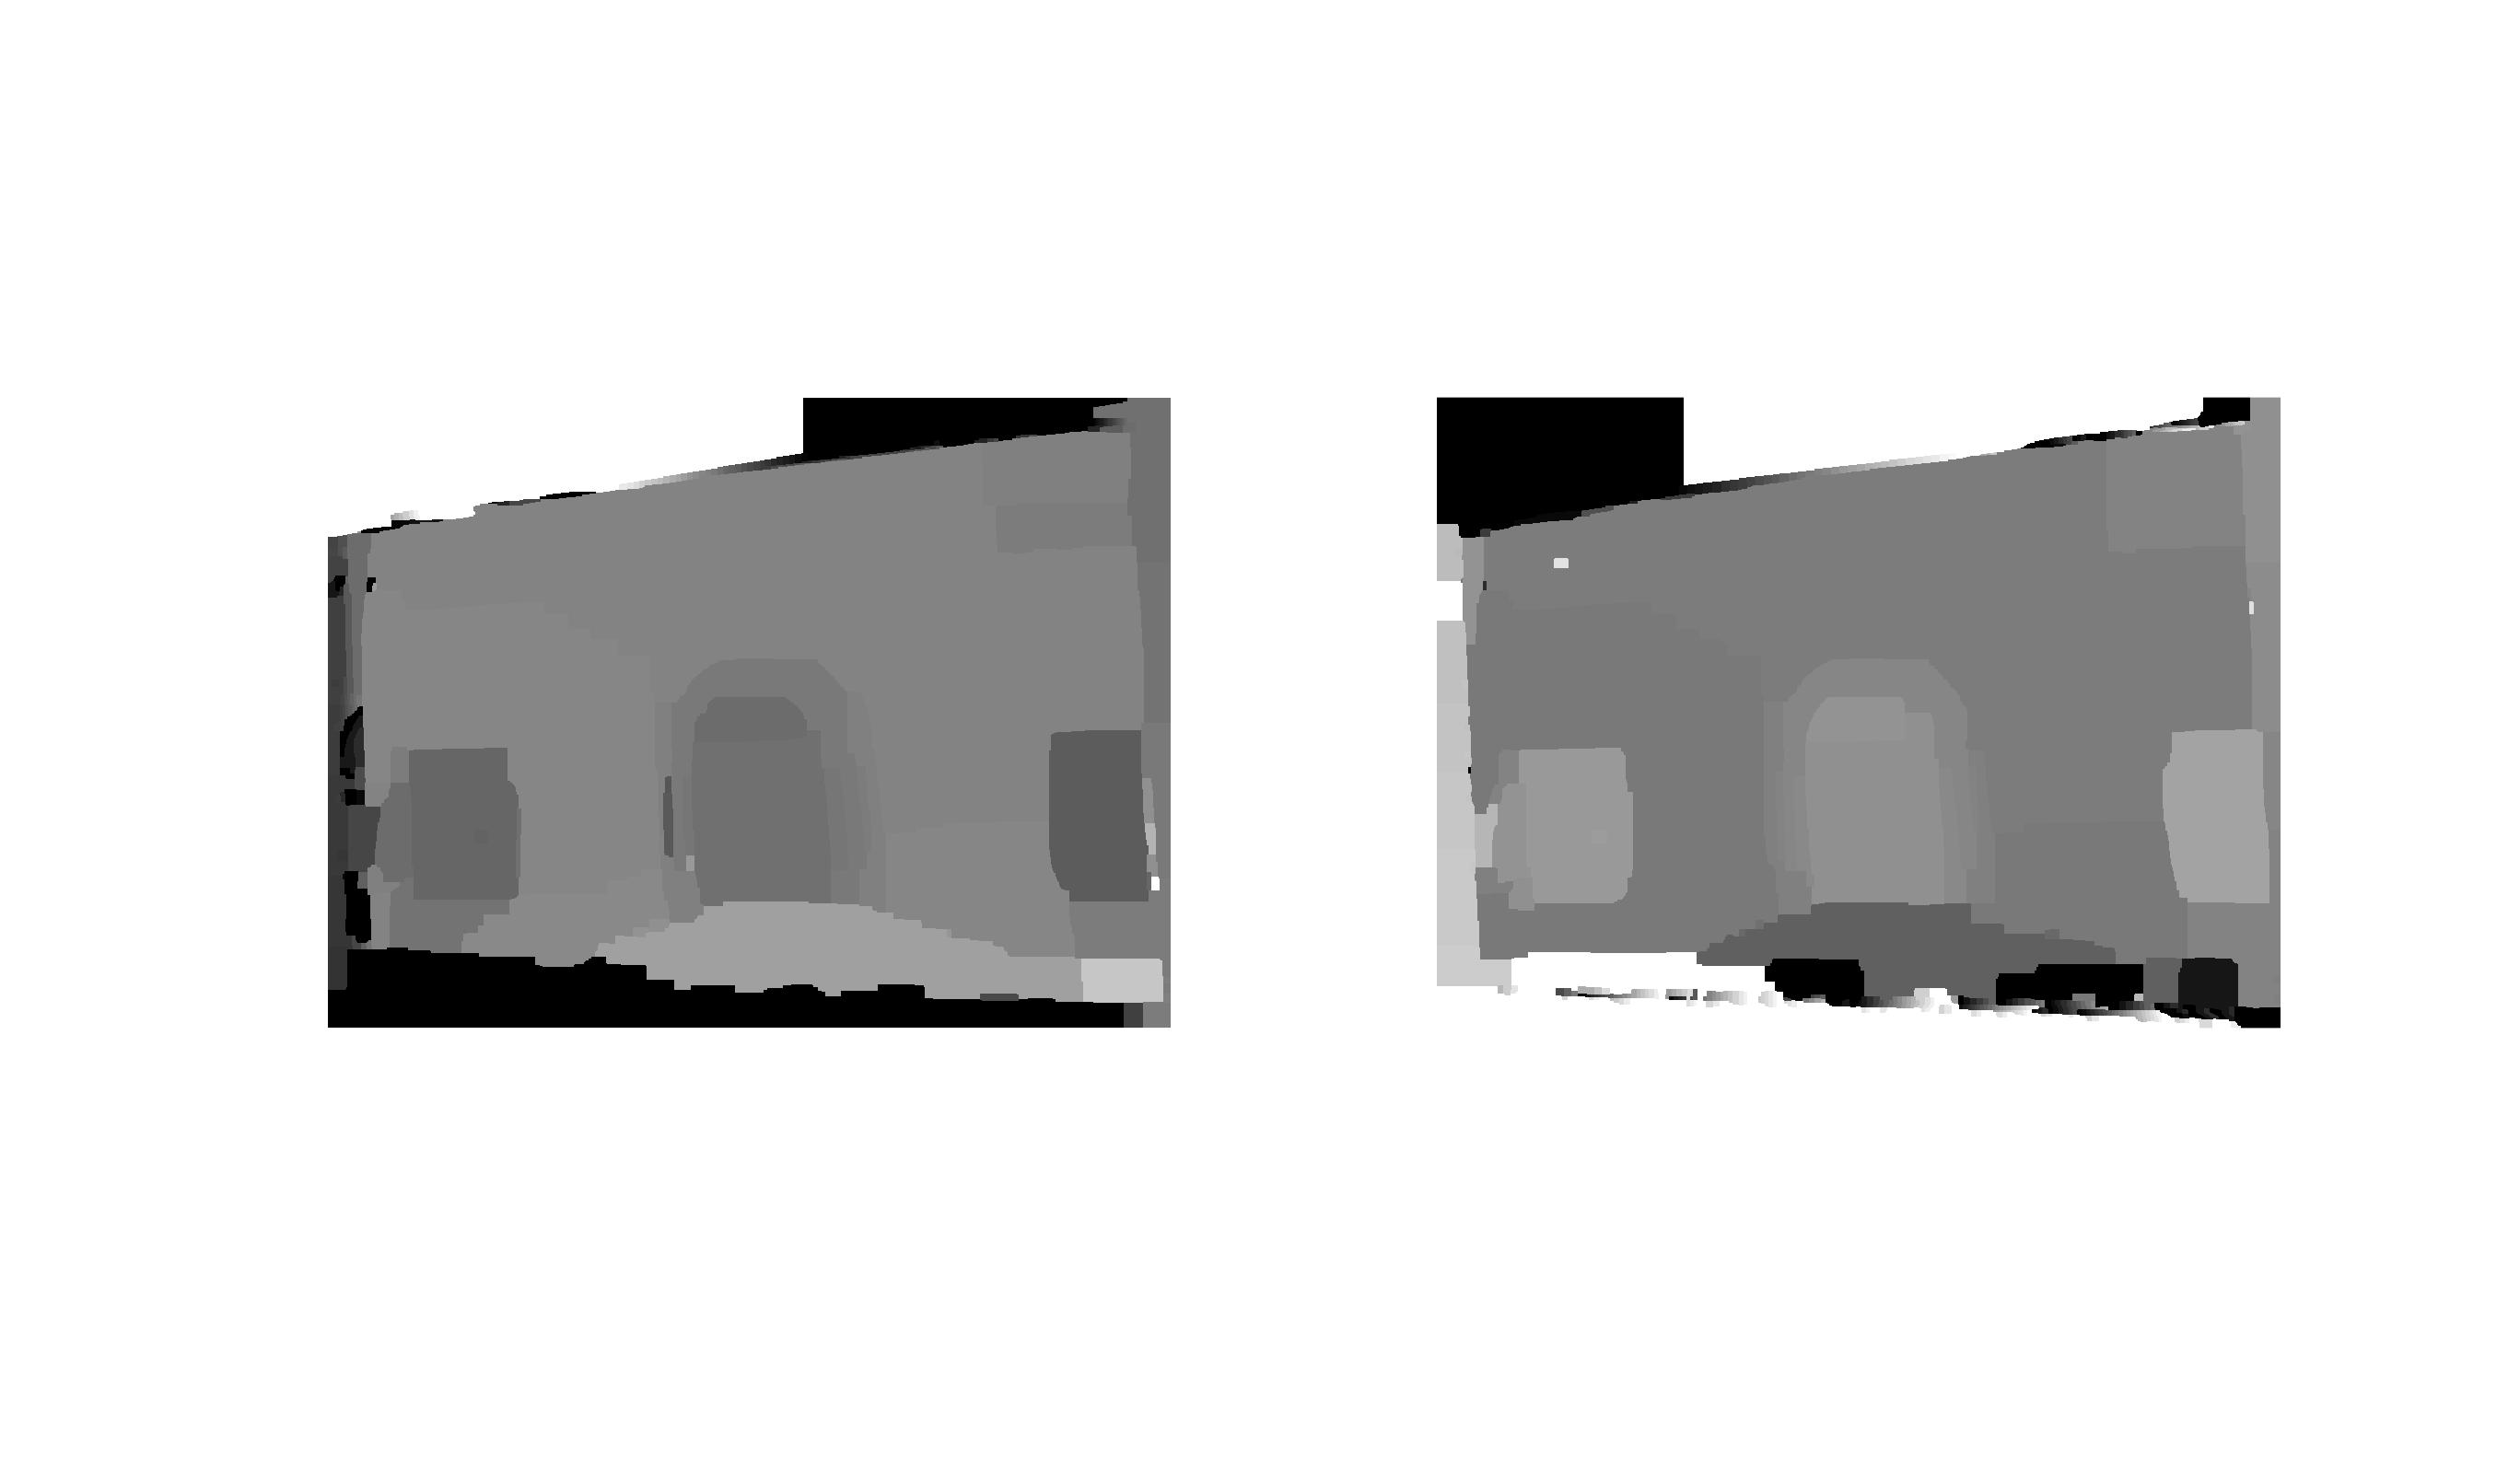
\includegraphics[width=1.1\textwidth]{gc_500_7_1.jpg}
	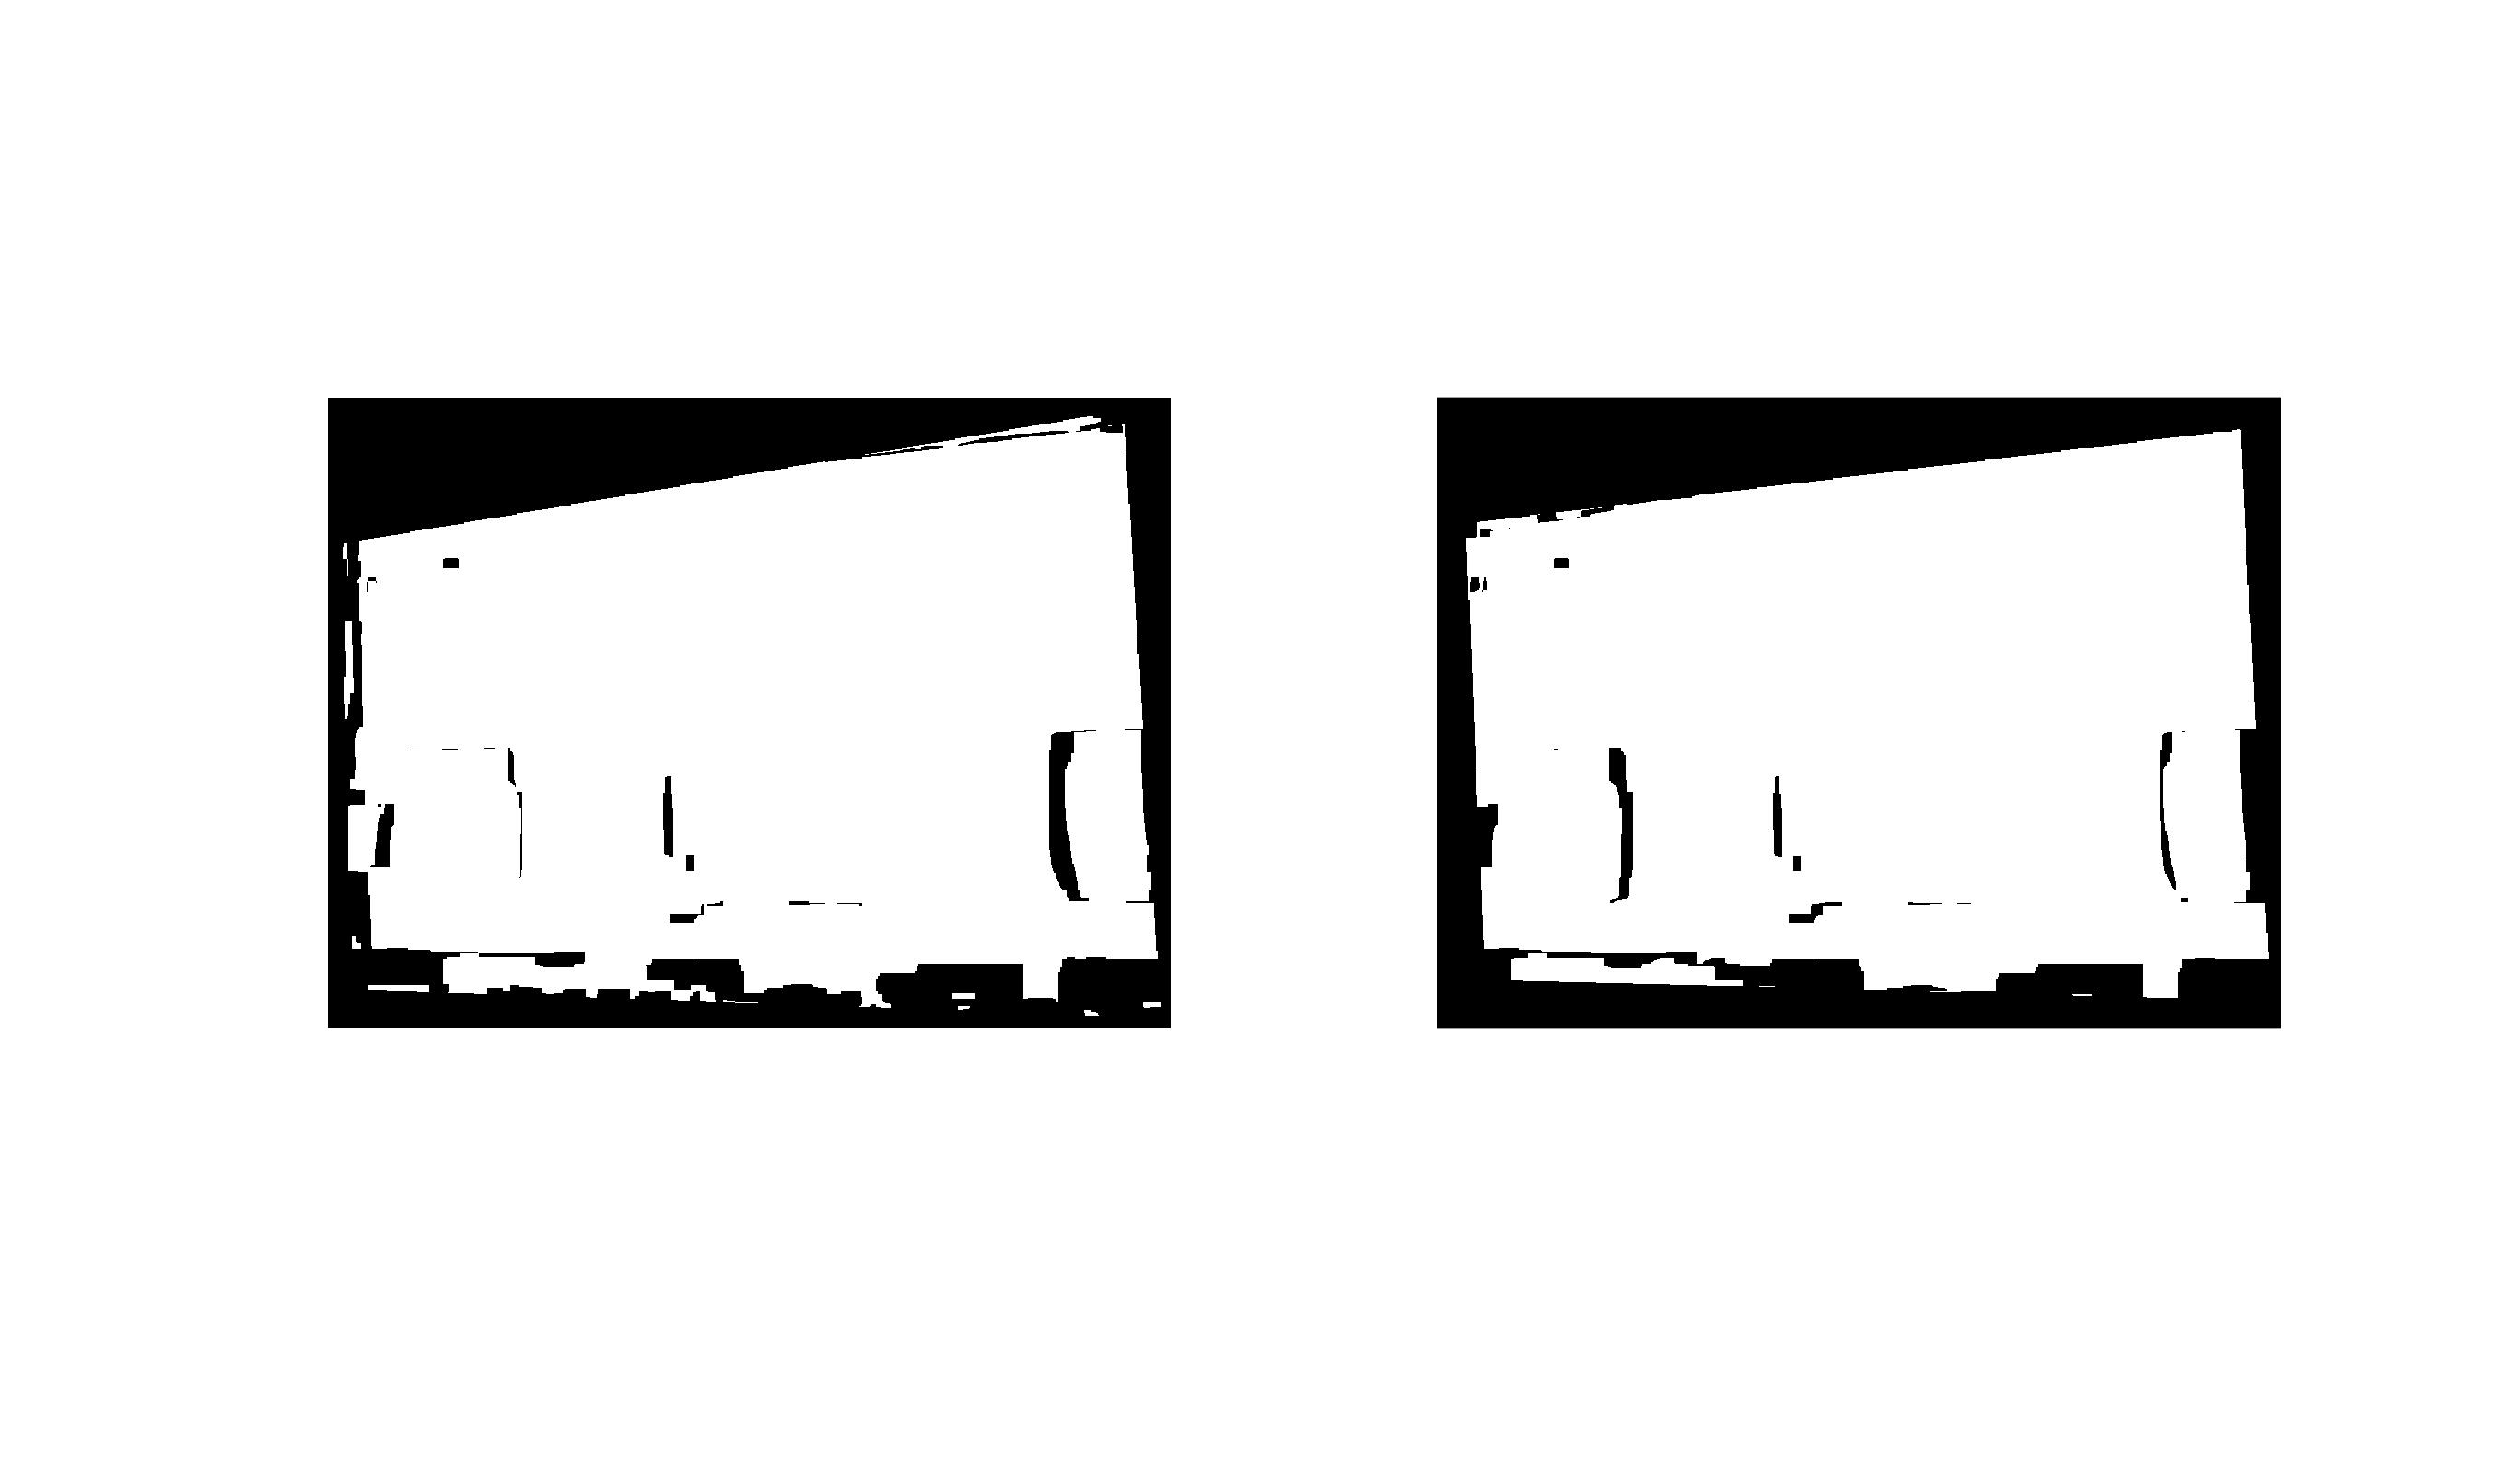
\includegraphics[width=1.1\textwidth]{gc_500_7_2.jpg}
	\caption{$DC*500$, $SC*7$}
	\label{fig1}
\end{figure}
Here the SC factor of 7 gives the most correctly mapped points. 

\begin{figure}[H]
	\centering
	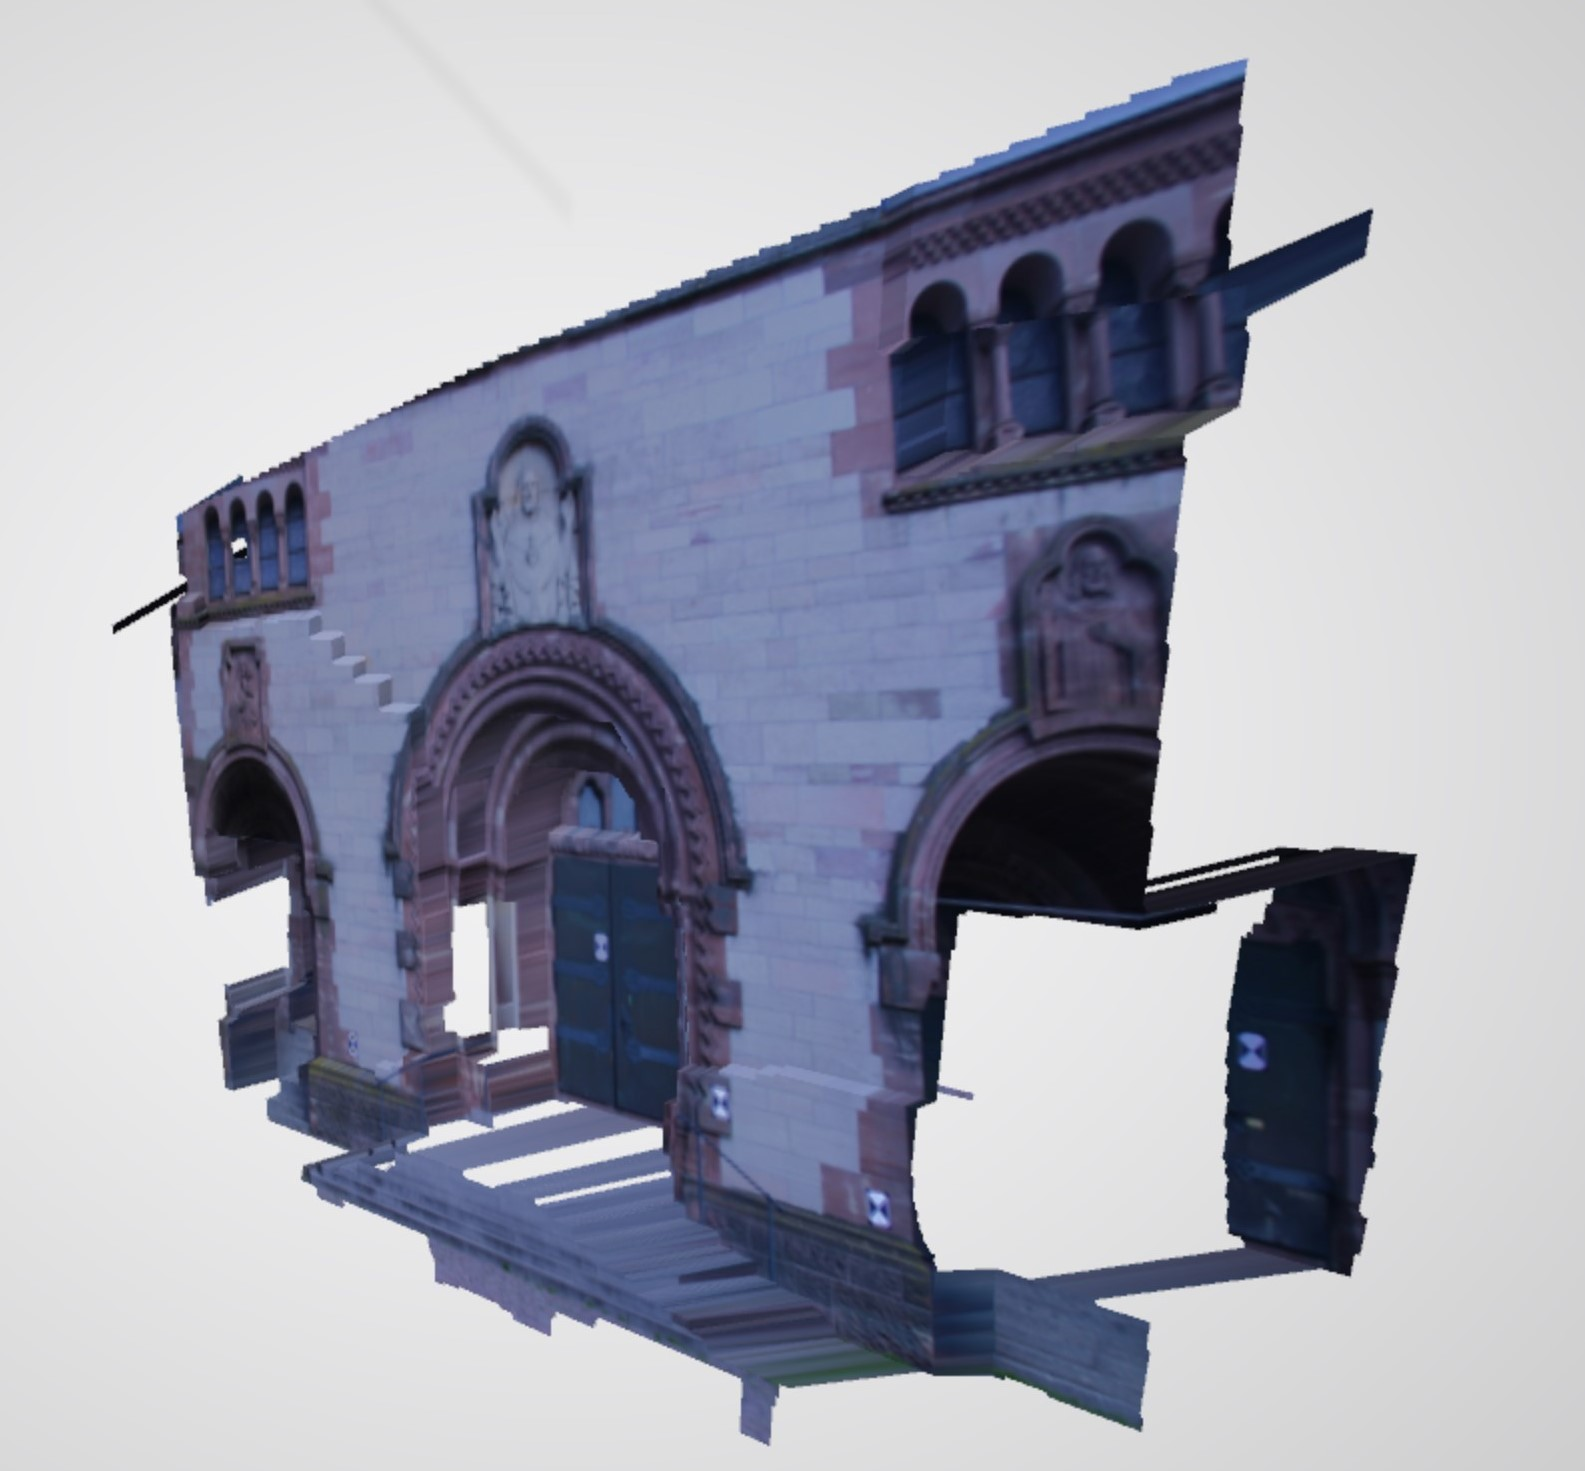
\includegraphics[width=0.6\textwidth]{gc_model_1.jpg}
	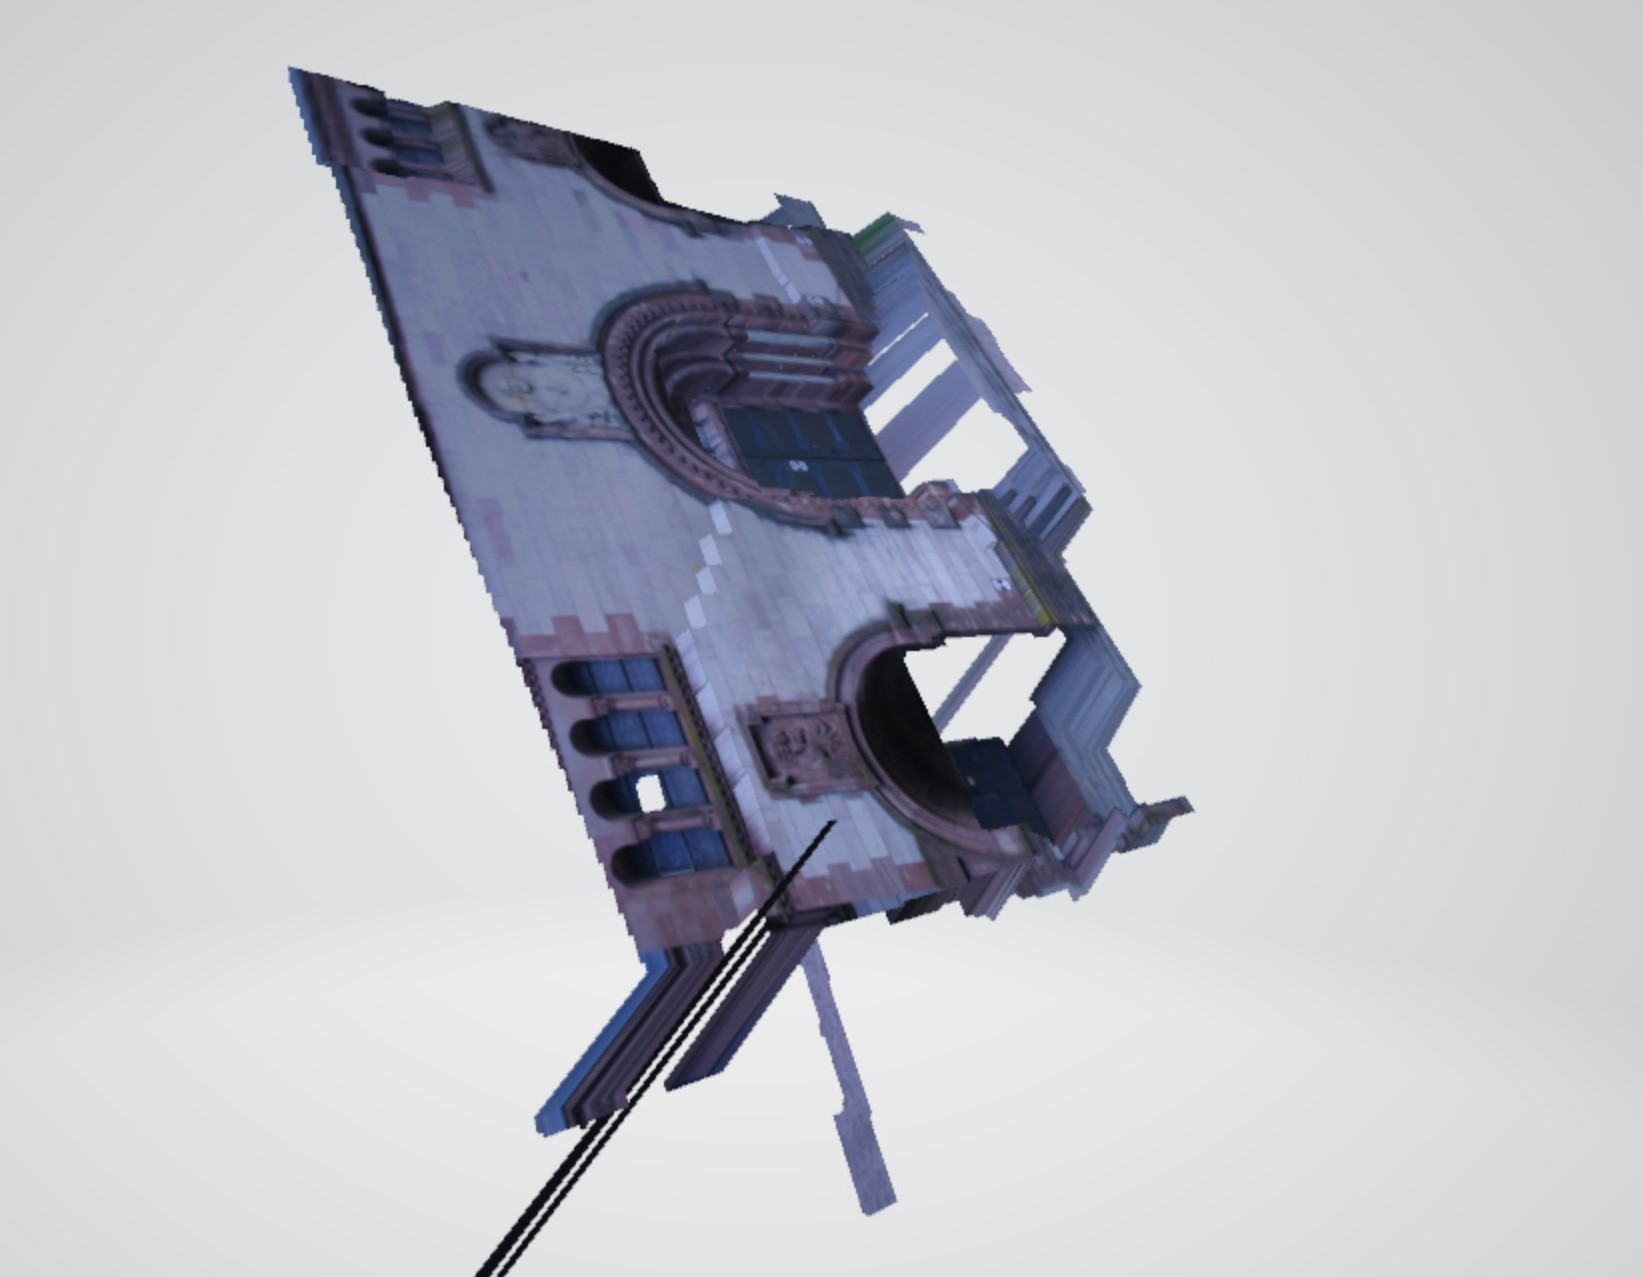
\includegraphics[width=0.6\textwidth]{gc_model_2.jpg}
	\caption{Textured 3D Model from Graph Cut with range $[-40, 40]$ and filter Window Size 7}
	\label{fig1}
\end{figure}

As can be seen this implementation works considerably better than the winner-takes-all stereo matching algorithm in smoothness. This time the flat surface of the wall is represented quite well and features such as the stair and the door are very well represented. Due to this algorithm beeing computationally more expensive finding the correct range is even more important. 

\section{Disparity Range Automation}

To calculate an automatic disparity range an approach using 8-point RANSAC was choosen. This algorithm, as was seen in previous exercises, returns a large set of point correspondences of the two images. This dataset was used to calculate the average distance in $x$ direction between matching points. From this we get a good measurement of how far the detected points, which are assumed to be points of interest, are apart. In manner of good engineering this average point distance is then multiplied by a safety factor (in this case choosen to be $2$ in this case) and set as the upper and lower boundaries of the range. As can be seen in the pictures below, this performs really well. For the provided image pair this algorithm resulted in an average range of $[-6, 6]$

\begin{figure}[H]
	\centering
	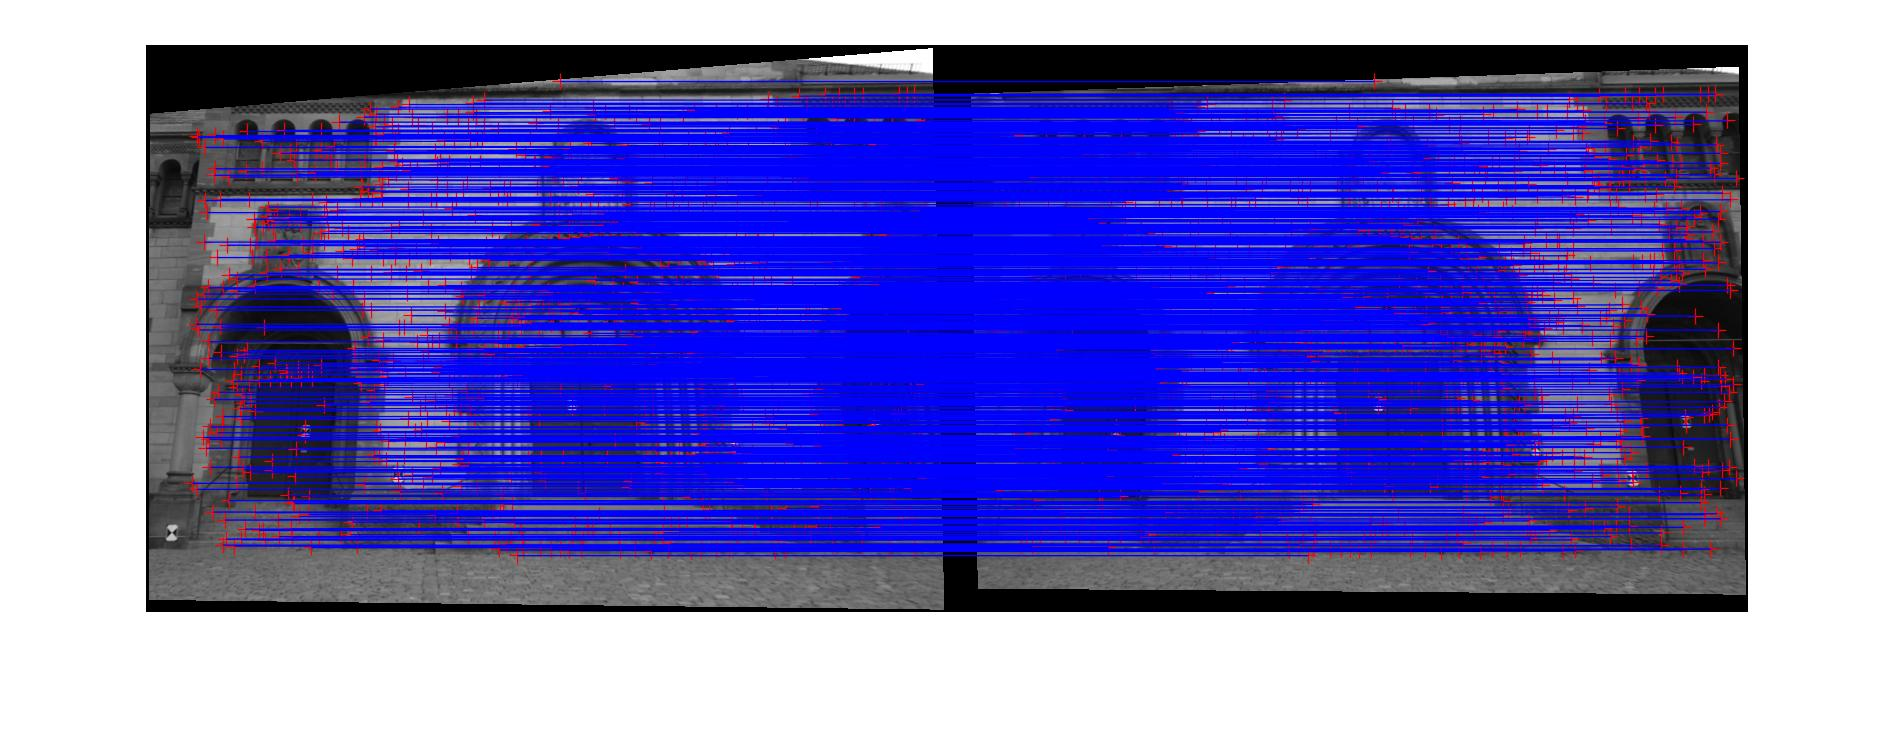
\includegraphics[width=1.1\textwidth]{8pRansac}
	\caption{8-Point RANSAC Matching of the two images}
	\label{fig1}
\end{figure}


This results in a much lower computation time for both algorithms. It can be imagined that such a method would not perform well if the distance between corresponding points varies a lot. This would be the case if it was tried to compute a disparity map of an object that varies in orders of magnitude more in distance from the camera.

\subsection{Disparity Computation}

For the disparity computation this range results in a way better performance in the amount of correctly mapped points, especially on the flat stone wall. The smaller range also decreases the possible space for mismatches.   

\begin{figure}[H]
	\centering
	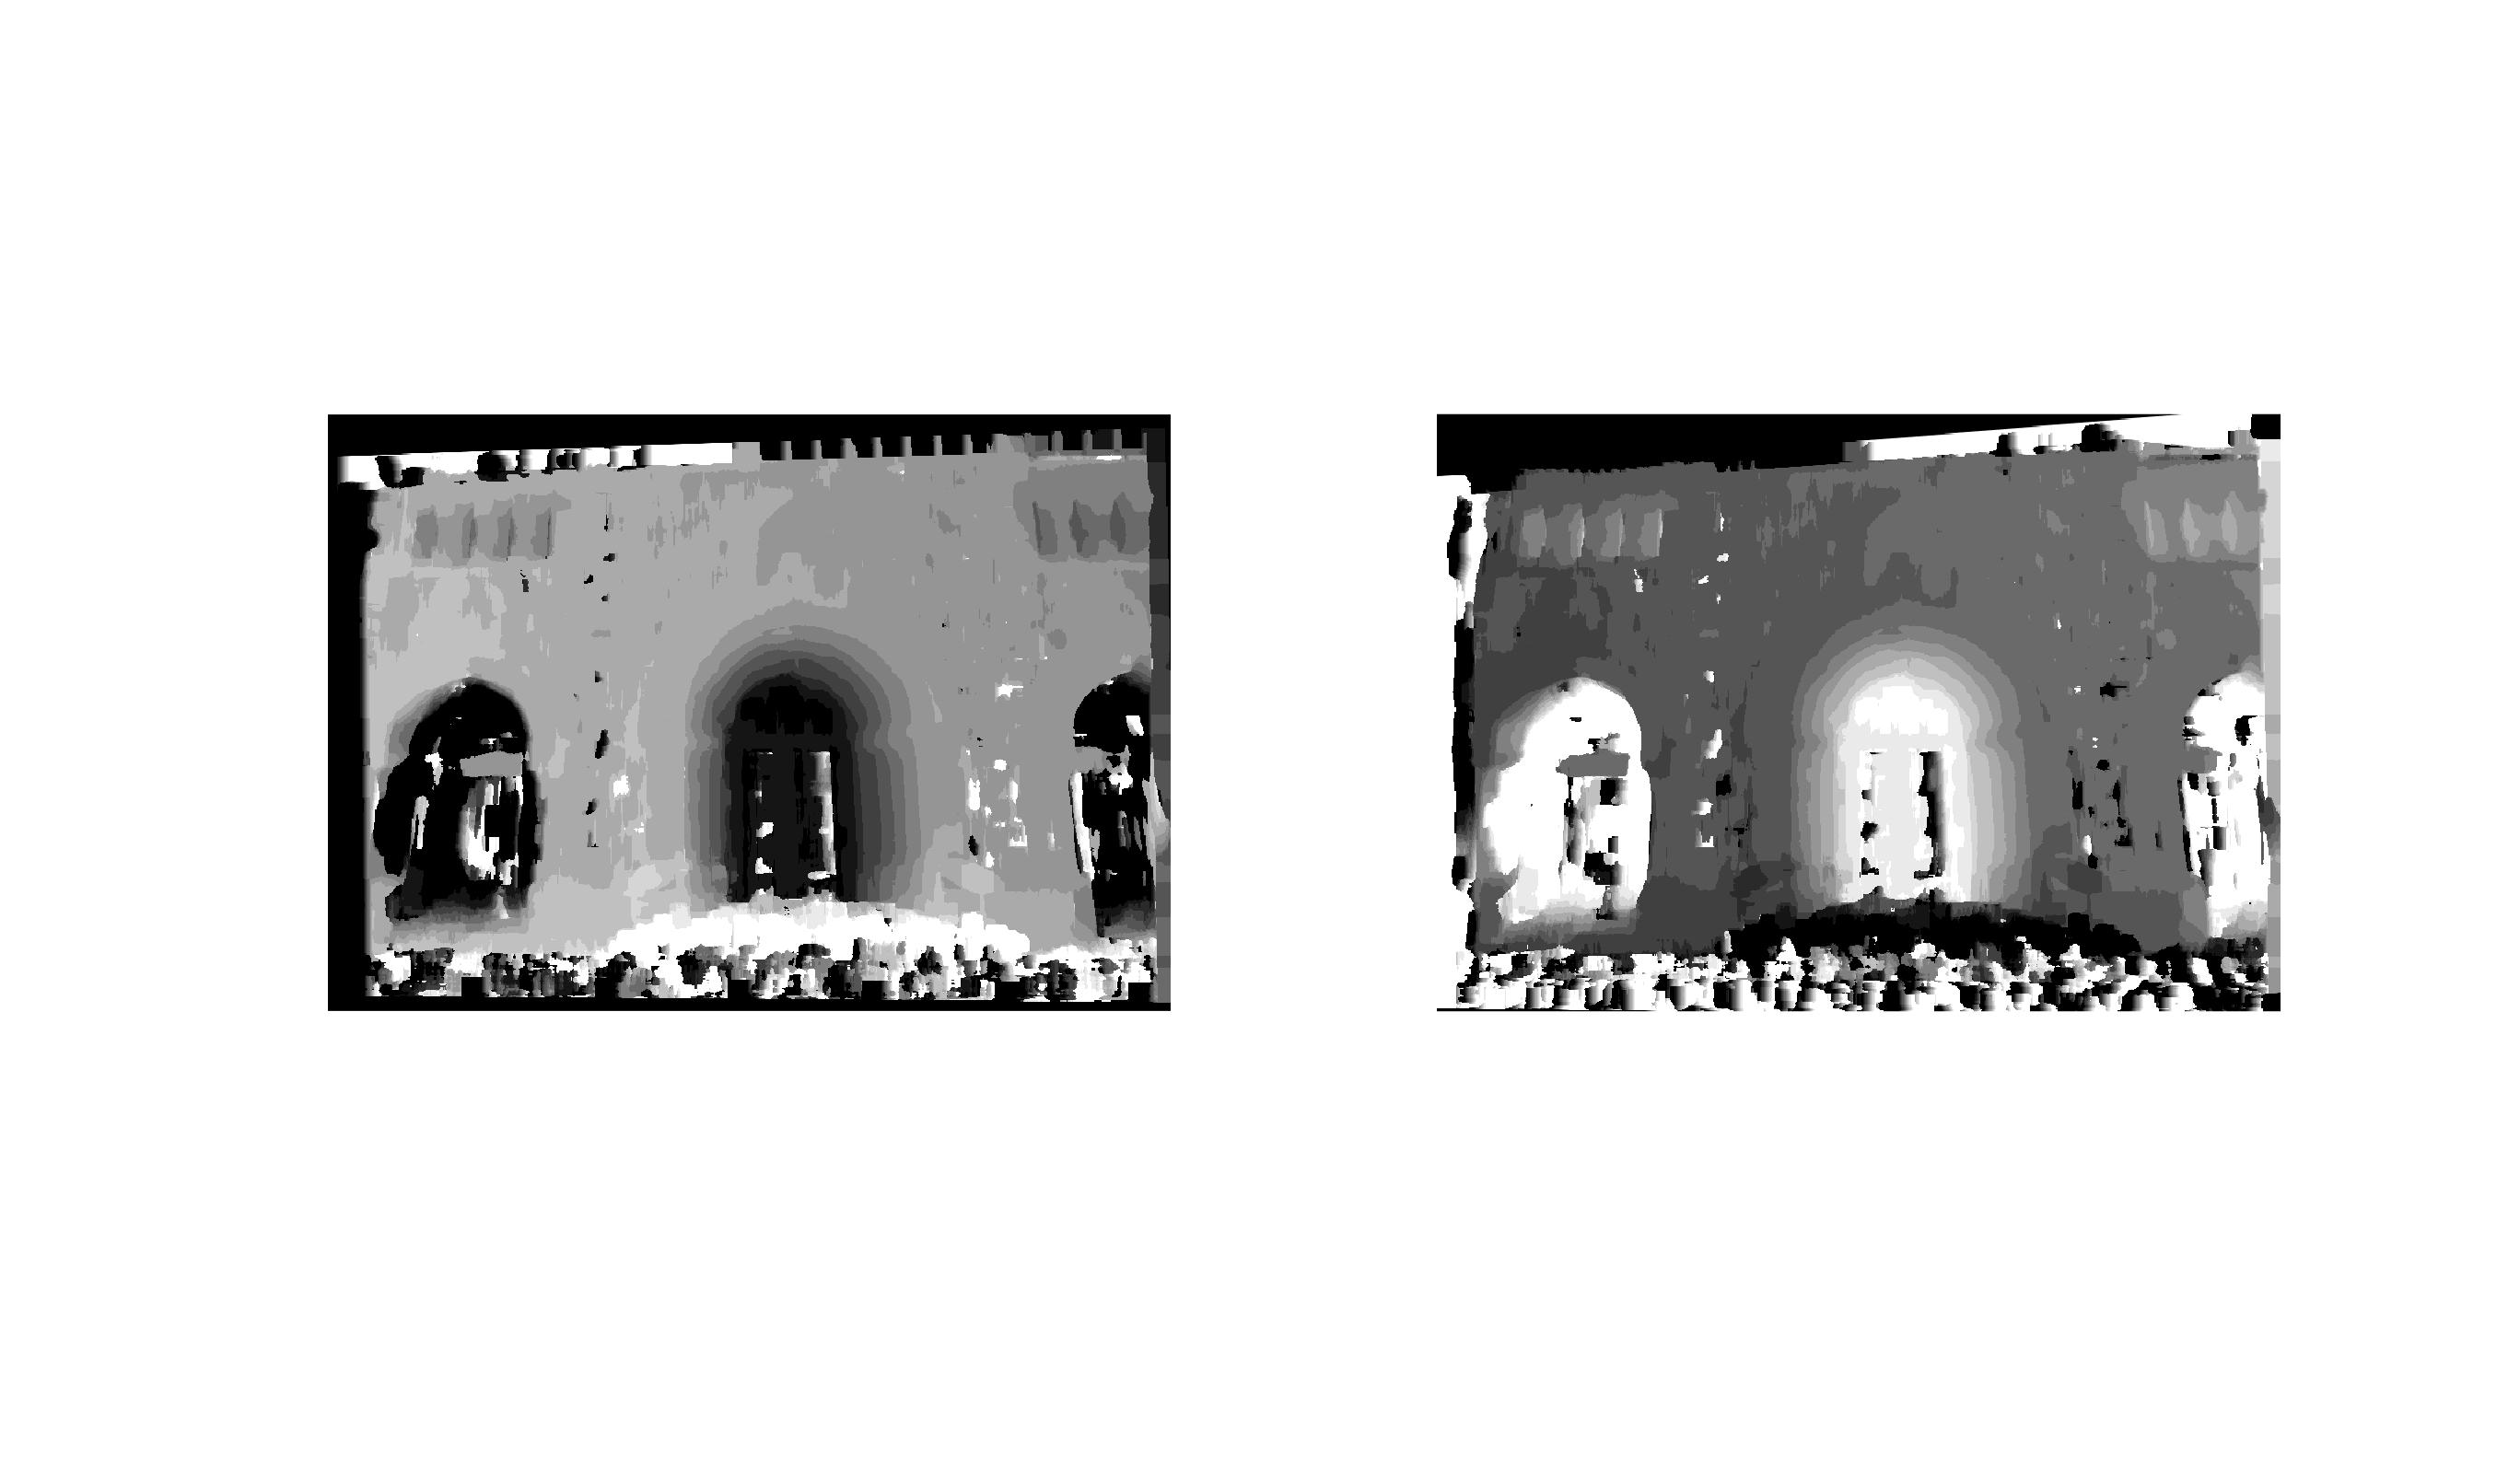
\includegraphics[width=1.1\textwidth]{1.jpg}
	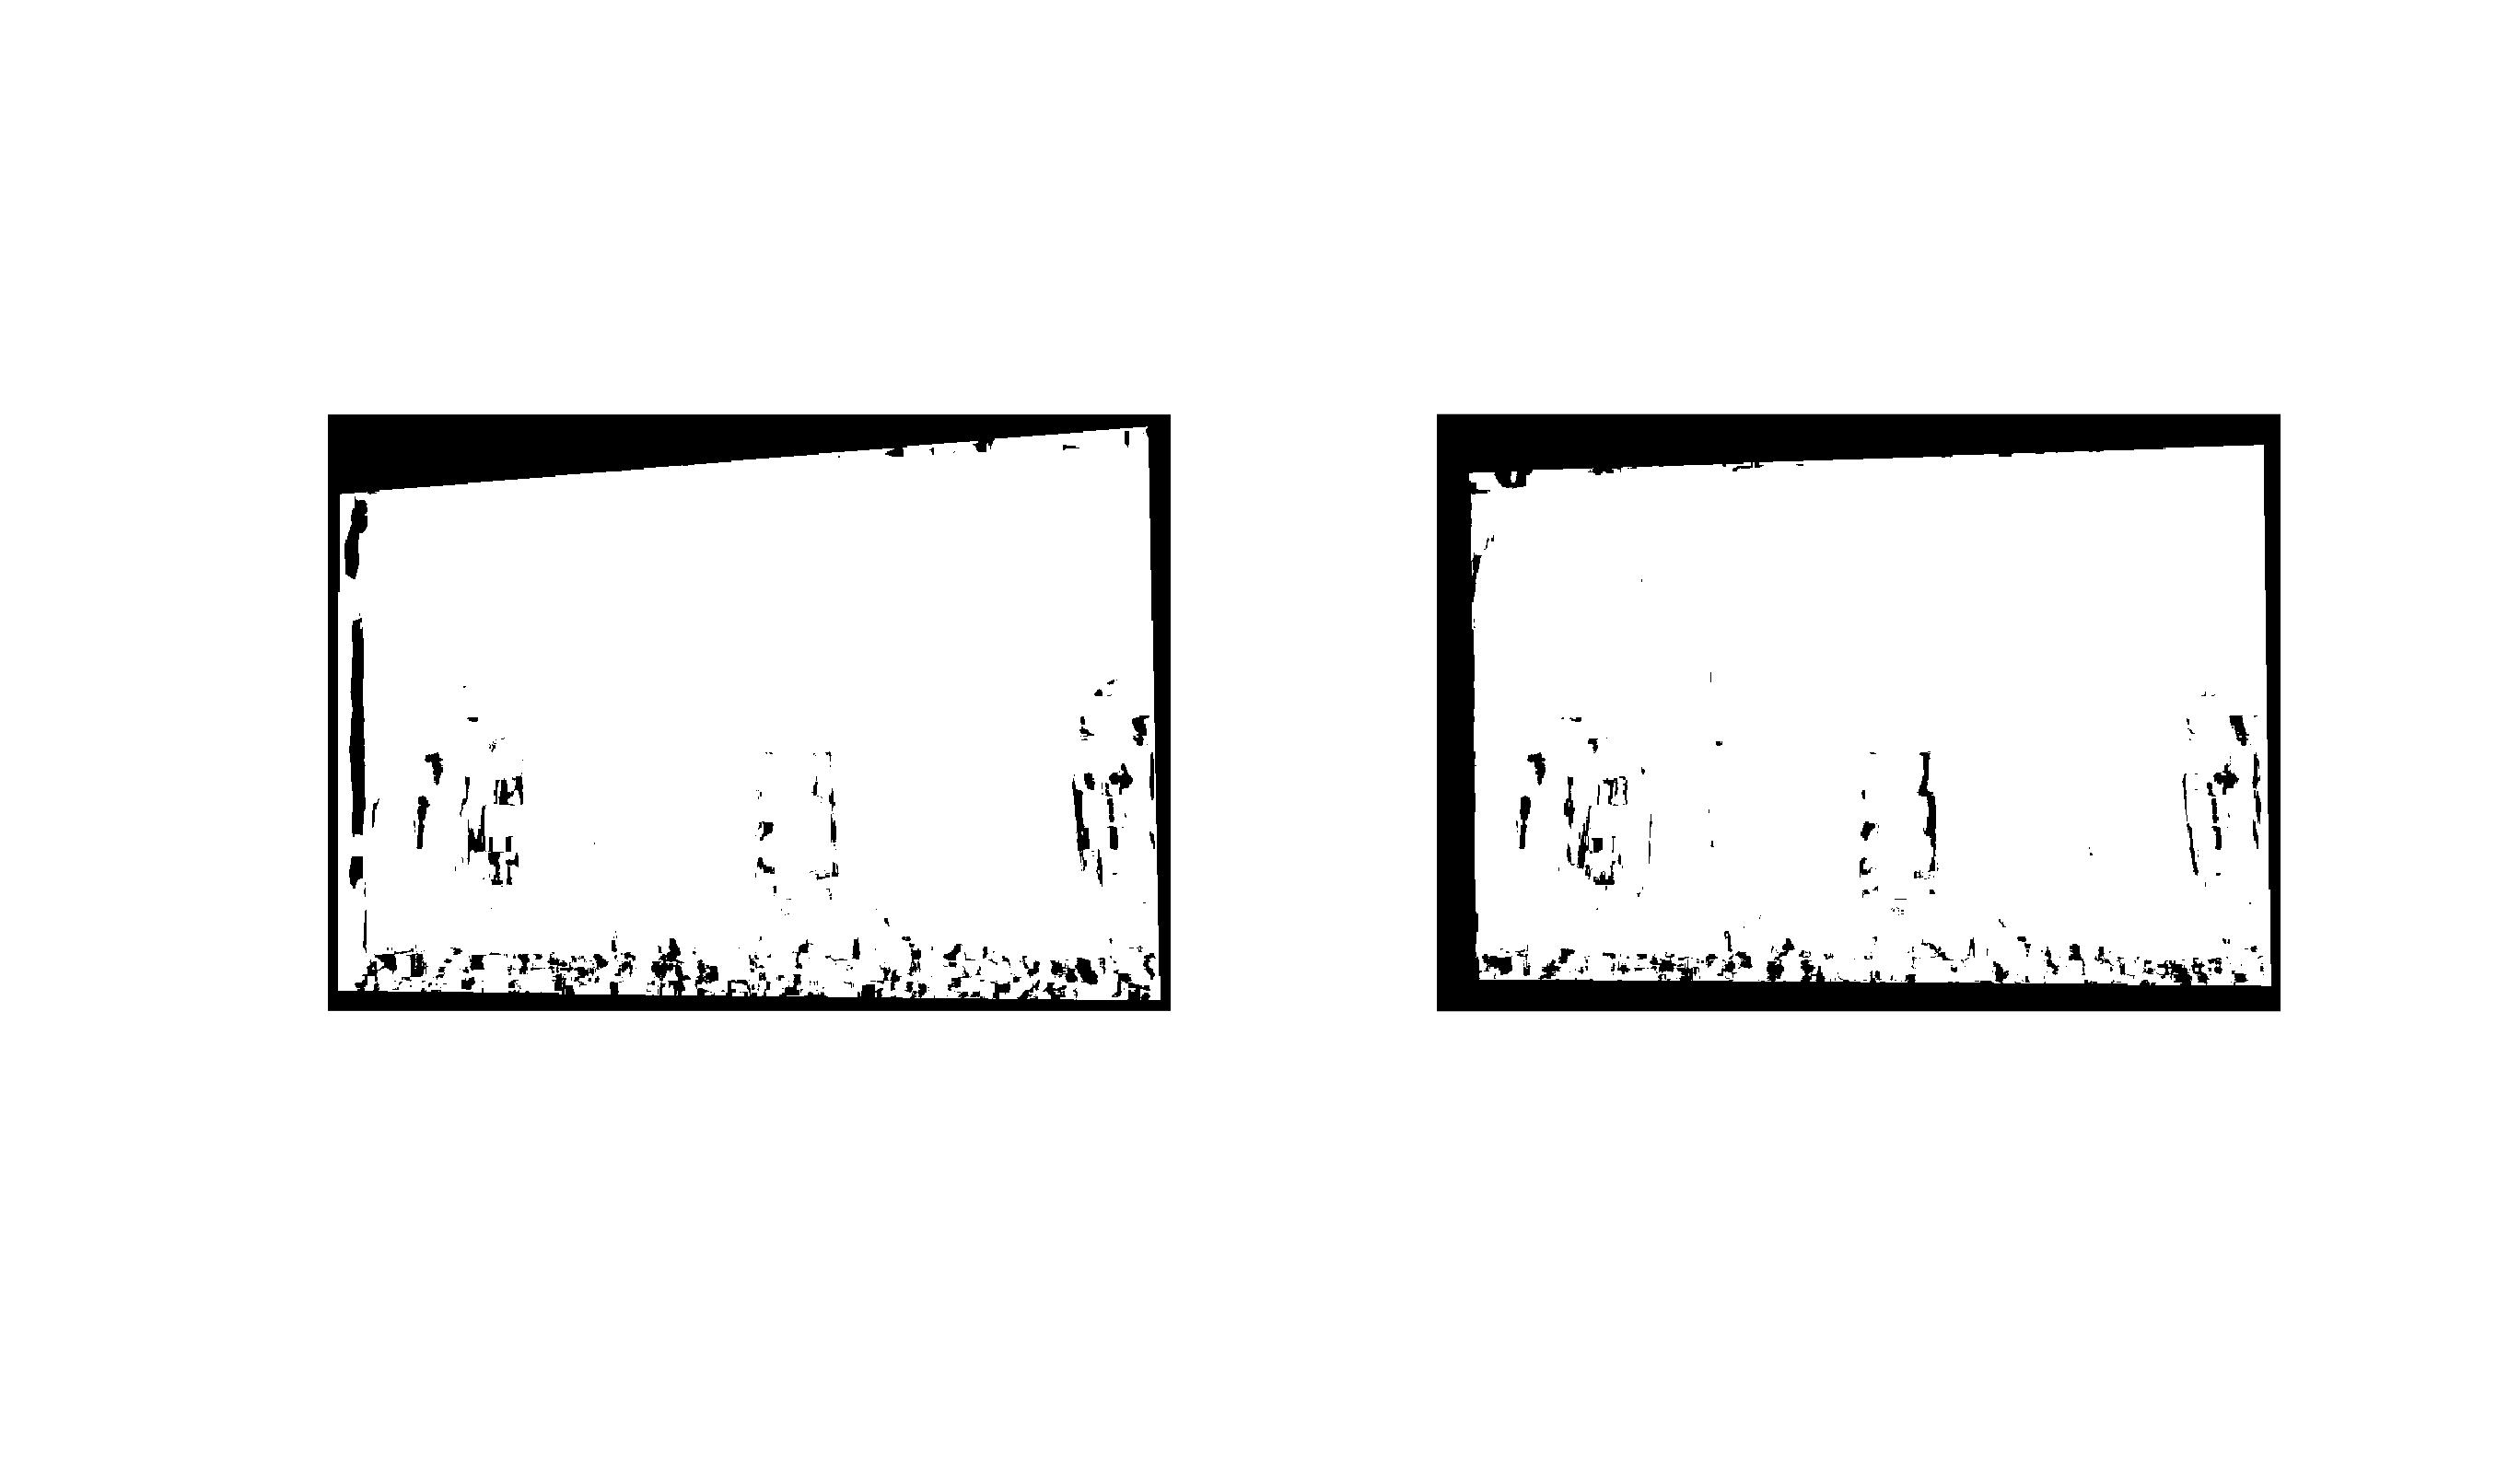
\includegraphics[width=1.1\textwidth]{2.jpg}
	\caption{19x19 Filter Window and range $[-6,6]$}
	\label{fig1}
\end{figure}
\begin{figure}[H]
	\centering
	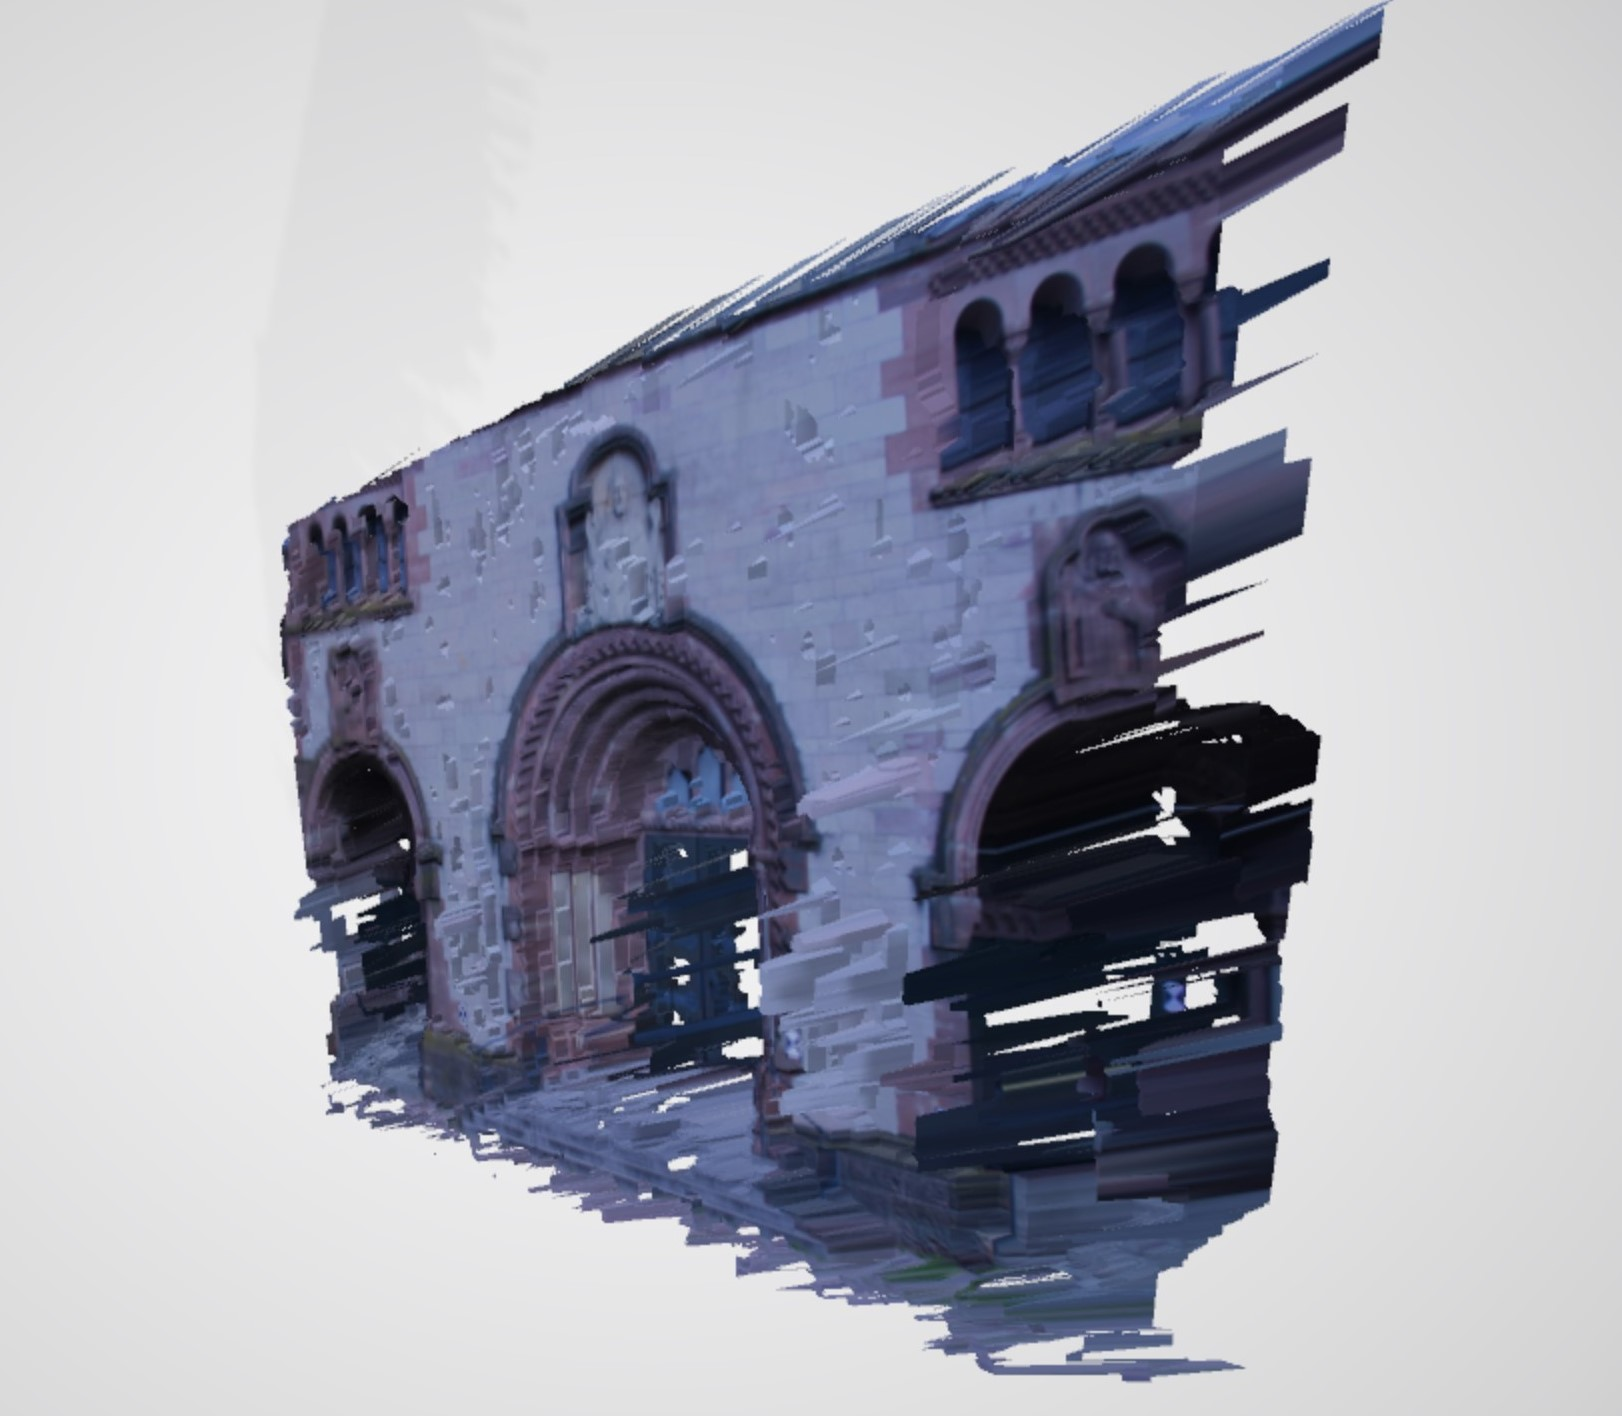
\includegraphics[width=0.8\textwidth]{5.jpg}
	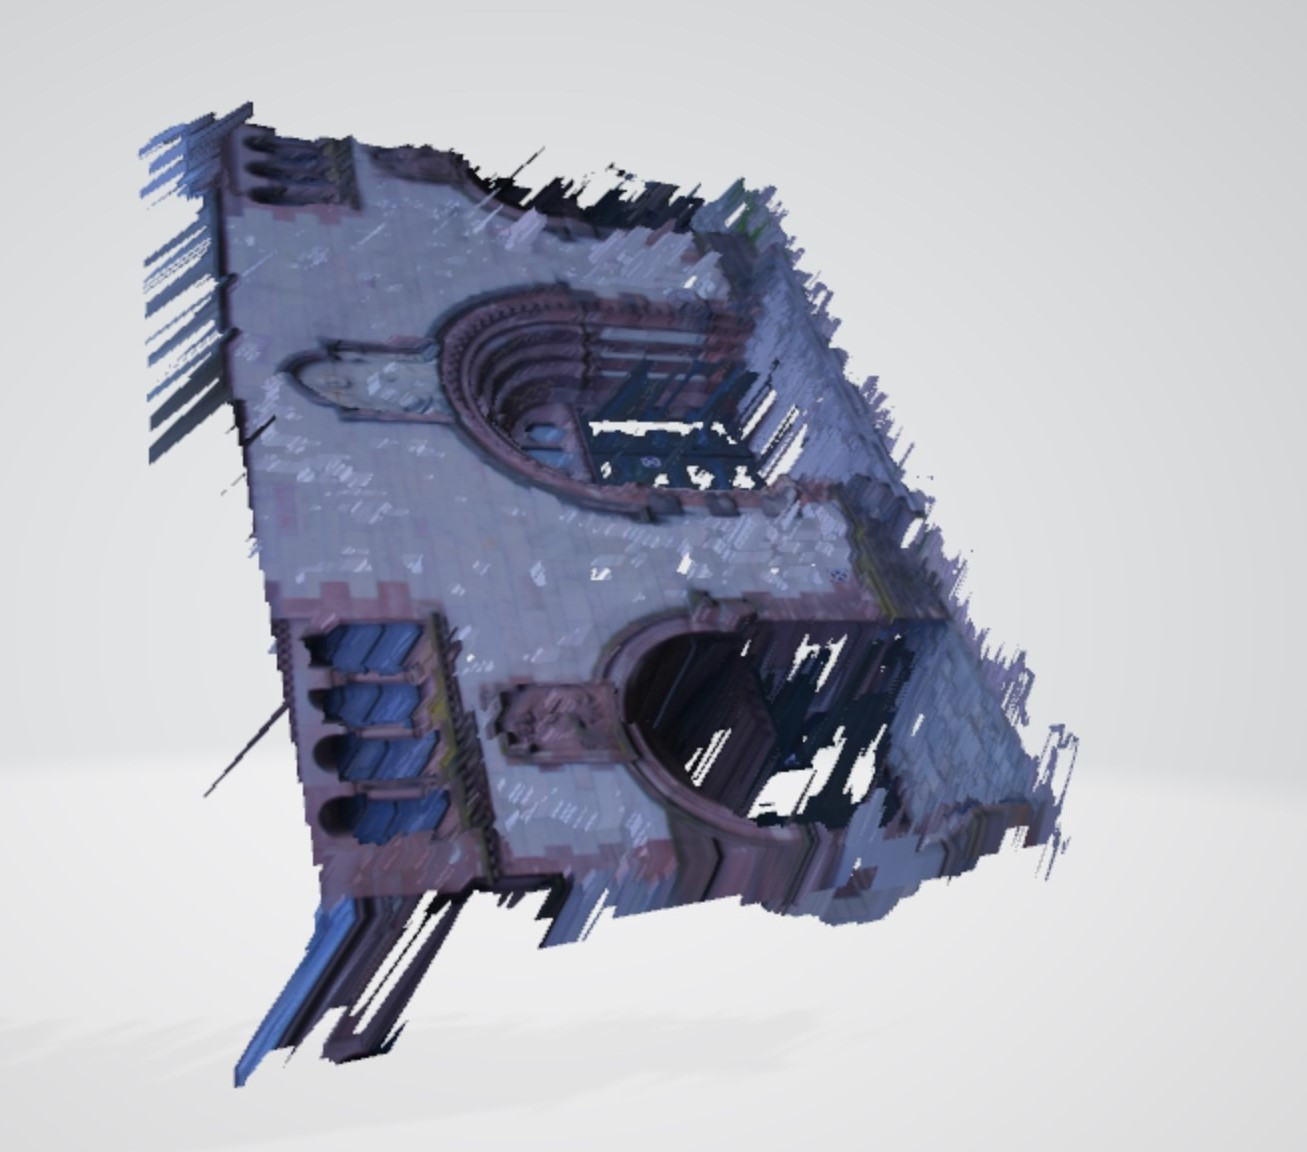
\includegraphics[width=0.8\textwidth]{6.jpg}
	\caption{Corresponding 3D Model}
	\label{fig1}
\end{figure}

\subsection{Graph Cut}
This model is looking great! Also on the graph cut algorithm the reduced range performs very well for the reasons already named. 

\begin{figure}[H]
	\centering
	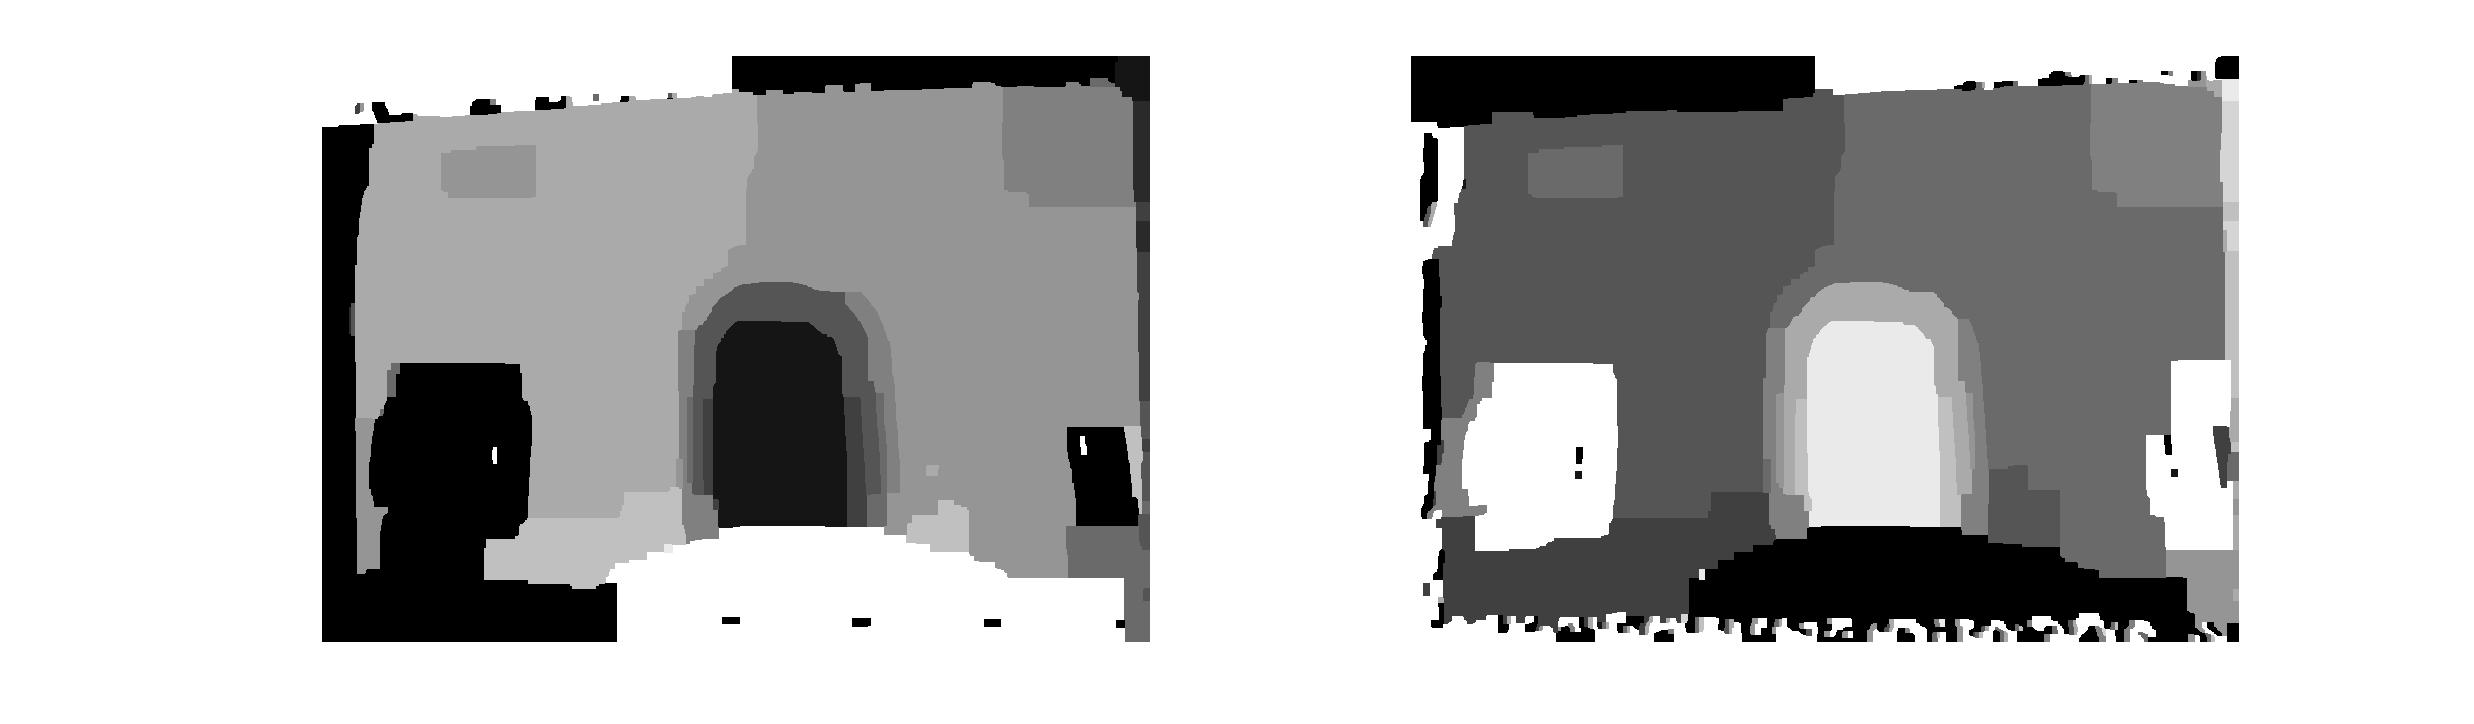
\includegraphics[width=1.1\textwidth]{3.jpg}
	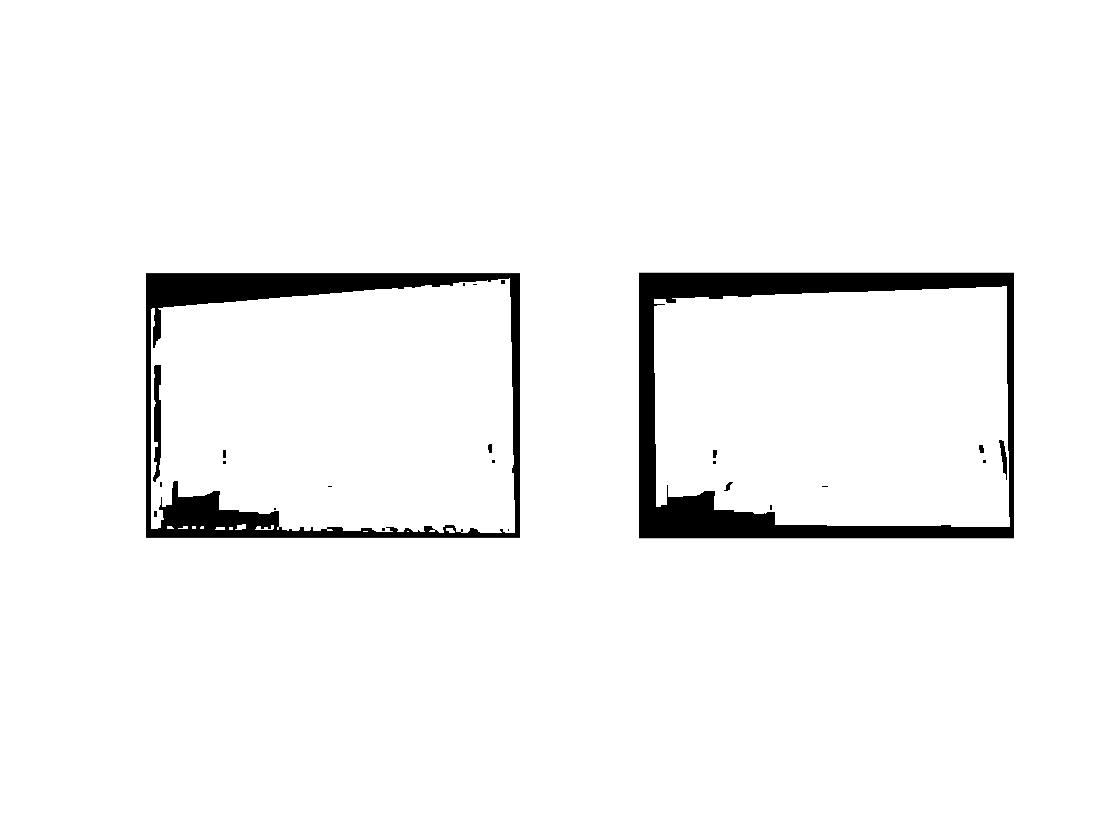
\includegraphics[width=1.1\textwidth]{4.jpg}
	\caption{$DC*500$, $SC*7$ and range $[-6, 6]$}
	\label{fig1}
\end{figure}
\begin{figure}[H]
	\centering
	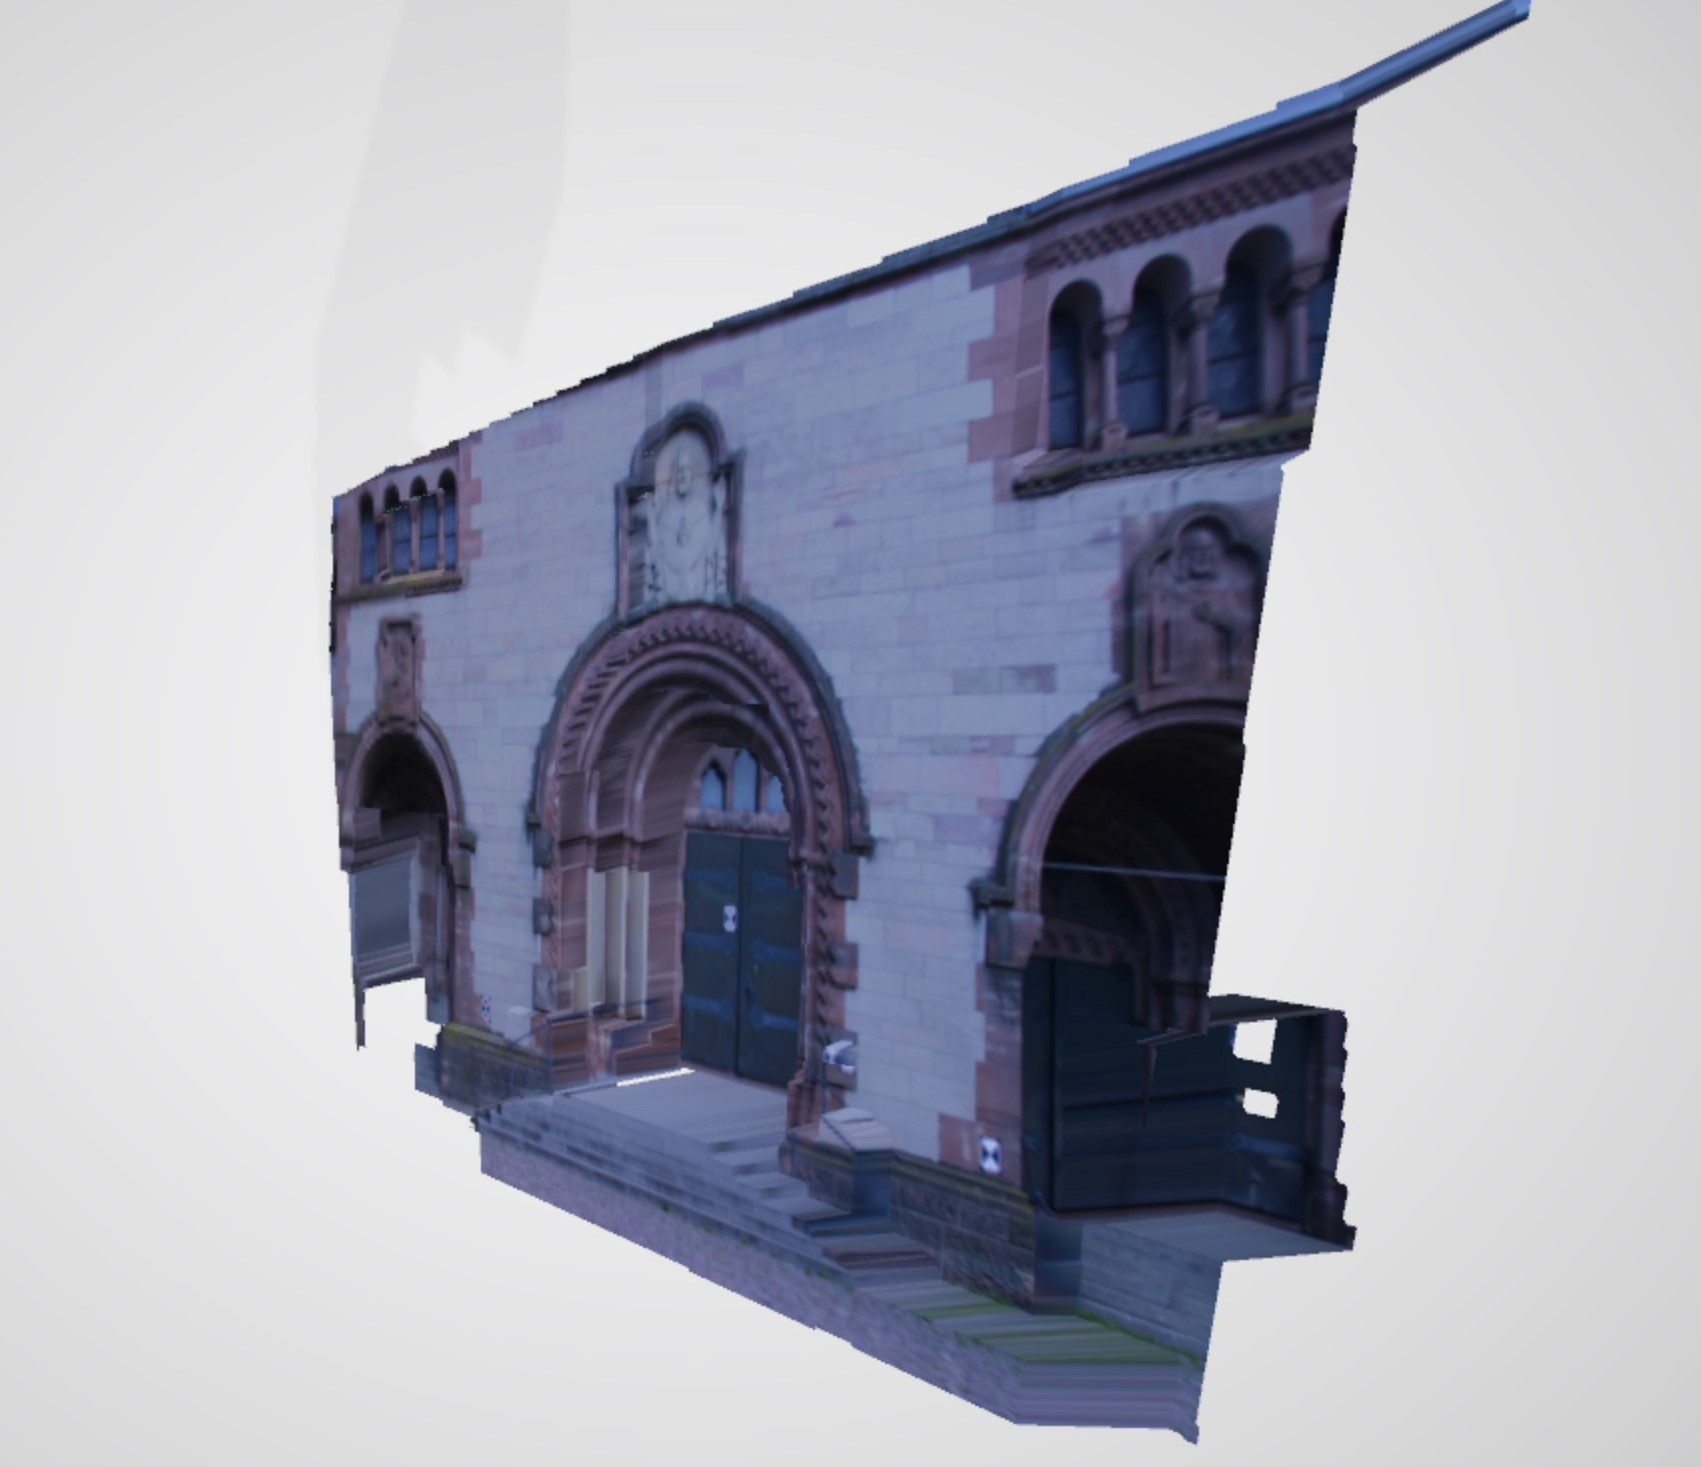
\includegraphics[width=0.8\textwidth]{7.jpg}
	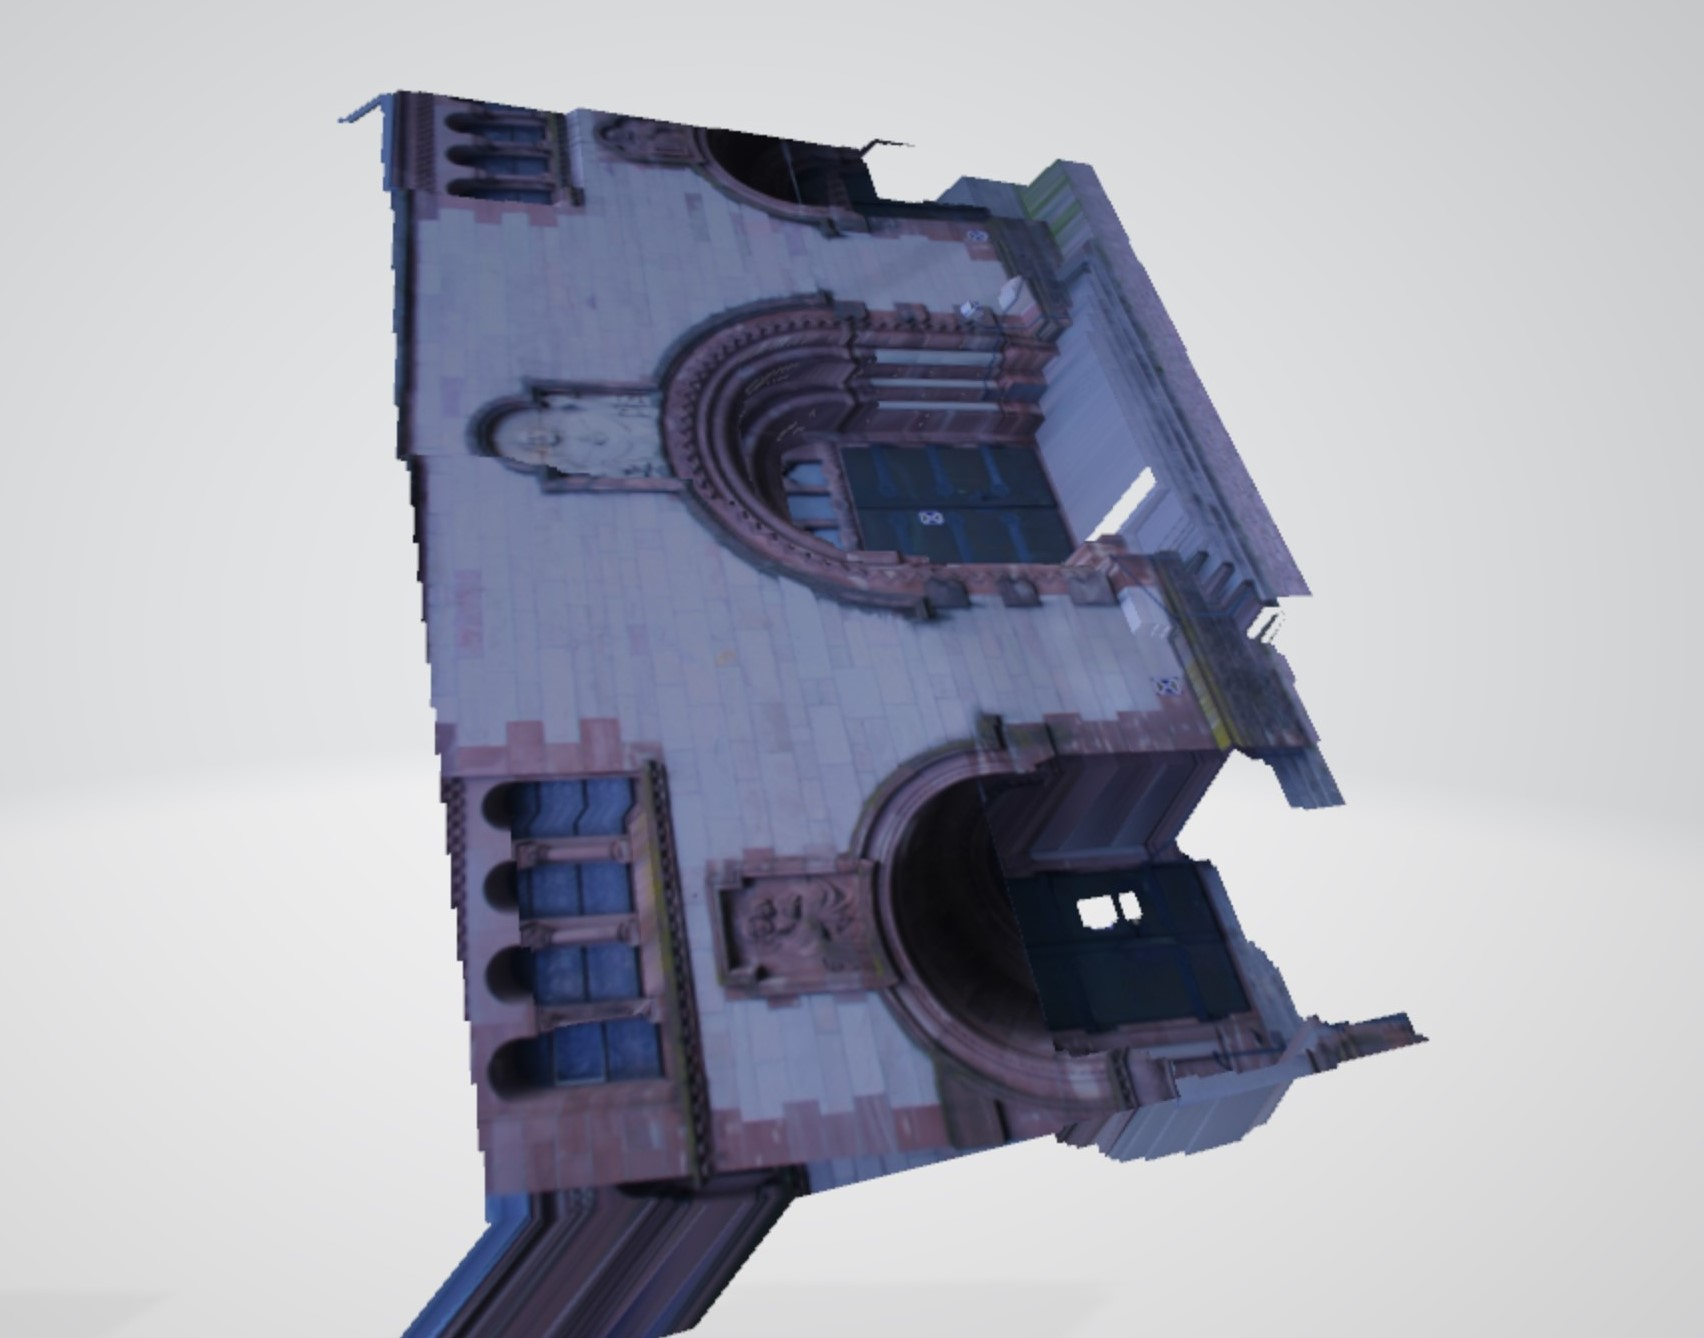
\includegraphics[width=0.8\textwidth]{8.jpg}
	\caption{Corresponding 3D Model}
	\label{fig1}
\end{figure}



\end{document}